\documentclass[11pt]{article}
\usepackage[utf8]{inputenc}
\usepackage[tbtags]{amsmath}
\usepackage{amsthm}
\usepackage{mathtools}
\usepackage{amssymb}
\usepackage{amsfonts}
\usepackage[english]{babel}
\usepackage{hyperref}
\usepackage{float}
\usepackage{bm}
\usepackage{graphicx}
\usepackage{subfigure}
\usepackage{multirow}
\usepackage{geometry}
\usepackage{multicol}
\usepackage{tabu}
\usepackage{longtable}
\usepackage{csquotes}
\usepackage[linesnumbered,ruled,vlined]{algorithm2e}
\usepackage[backend=biber,style=ieee,sorting=nty]{biblatex}
\allowdisplaybreaks

\hypersetup{
    colorlinks=true,
    linkcolor=blue,
    filecolor=magenta,      
    urlcolor=cyan,
}

\newtheorem{theorem}{Theorem}
\newtheorem{lemma}{Lemma}[section]
\newtheorem{definition}{Definition}[section]
\newtheorem{proposition}{Proposition}
\newtheorem{corollary}{Corollary}[section]
\newtheorem{remark}{Remark}

\SetKwInput{KwInput}{Input}
\SetKwInput{KwOutput}{Output}
\SetKwInput{KwInit}{Initialization}

\DeclareMathOperator*{\argmin}{arg\,min}
\DeclareMathOperator*{\argmax}{arg\,max}

\addbibresource{ref.bib}

\title{\bf Detection of Multiple Change Points in Heterogeneous Panel Vector Autoregressive Models}
\author{Peiliang Bai, Abolfazl Safikhani, George Michailidis}
%\date{September 15 2021}

\begin{document}

\maketitle
\begin{abstract}
    [TO BE CONTINUED...]
\end{abstract}

\section{Introduction}
[TO BE CONTINUED...]


\section{Single Change Point Model and Detection Strategies}\label{sec:single-cp}
\subsection{Model formulation}
Suppose we have $M$ subjects $\{X_t^i\}$ for $i=1,2,\dots, M$, which are $p$-dimensional VAR($d_i$) time series with $T$ observations, where $d_i \geq 1$ is the lag. For each time series, there exists a single change point $\tau_i$ such that $\tau_i \in \{1,2,\dots, T\}$ for $i=1,2,\dots, M$. The model is formulated as follows:
\begin{equation}
    \label{eq:1}
    \begin{aligned}
        X_t^i &= A_{1,1}^iX_{t-1}^i + A_{1,2}^iX_{t-2}^i + \cdots + A_{1,d_i}^iX_{t-d_i}^i + \epsilon_t^i, \quad t \leq \tau_i, \\
        X_t^i &= A_{2,1}^iX_{t-1}^i + A_{2,2}^iX_{t-2}^i + \cdots + A_{2,d_i}^iX_{t-d_i}^i + \epsilon_t^i, \quad t > \tau_i,
    \end{aligned}
\end{equation}
where the model parameter matrices $A_{1,q}^i$ and $A_{2,q}^i$ represent the transition matrices for the left-hand side and right-hand side of $\tau_i$ at lag $q$, both of them are sparse matrices with sparsity level equal to $s_{1,q}^i$ and $s_{2,q}^i$, and let $s_j^i \overset{\text{def}}{=} \sum_{q=1}^{d_i}s_{j,q}^i$ be the sparsity level for the matrix $\mathbf{A}_j^i \overset{\text{def}}{=} (A_{j,1}^i, A_{j,2}^i, \cdots, A_{j,d_{i}}^i) \in \mathbb{R}^{p \times d_ip}$, for $j=1,2$, and we assume that $s_j^i \ll p^2$ as well as the maximum sparsity level is defined as $s_{\max} \overset{\text{def}}{=} \max_{1\leq i \leq M}\max_{j=1,2}\sum_{q=1}^{d_i} s_{j,q}^i$. Moreover, denote that the true change points for all subjects are in a set $\mathcal{T} \overset{\text{def}}{=} \{\tau_1, \tau_2, \dots, \tau_M\}$, and we assume that the change points in $\mathcal{T}$ are close.


%\textcolor{magenta}{We need to be more clear of what we assume as the DGP for the CPs. We do not have \textit{common} CP, but that the individual CPs are close}

We denote the center of $\mathcal{T}$ as $\tau^\star$, and it is assumed that there exists a ball $\mathcal{B}(\tau^\star, r_T)$ covering the whole set $\mathcal{T}$, i.e. for each $\tau_i$, we have:
\begin{equation}
    \label{eq:2}
    \max_{1\leq i \leq M}|\tau_i - \tau^\star| \leq r_T,
\end{equation}
where $r_T > 0$ is the radius of the ball $\mathcal{B}$ and $r_T$ is a function of sample size $T$. Our goal is to estimate the center $\tau^\star$. 


\subsection{Detection algorithms}\label{sec:algorithms}
In this section, we establish two strategies based on the time lag of vector autoregressive models to detect change points. 
\subsubsection{Maximum lag detection strategy}\label{sec:max-lag}
Note that the lags might differ among all subjects, hence, the first strategy is
to consider the maximum lag $d \overset{\text{def}}{=} \max_{1\leq i \leq M}d_i$, and we expand all subjects to the lag $d$, and then by \cite{lutkepohl2005new} we can rewrite the $p$-dimensional VAR($d$) process in \eqref{eq:1} as a  $dp$-dimensional VAR(1) series as follows:
\begin{equation*}
    \begin{aligned}
        Y_t^i &= \mathbf{A}_1^iY_{t-1}^i + \widetilde{\epsilon}_t^i, \quad t \leq \tau_i, \\
        Y_t^i &= \mathbf{A}^i_2Y_{t-1}^i + \widetilde{\epsilon}_t^i, \quad t > \tau_i,
    \end{aligned}
\end{equation*}
where
\begin{equation*}
    Y^i_t = 
    \begin{pmatrix}
        X_t^i \\
        X_{t-1}^i \\
        \vdots \\
        X_{t-d+1}^i
    \end{pmatrix} \in \mathbb{R}^{pd},\ 
    \mathbf{A}_j^i = 
    \begin{pmatrix}
        A_{j,1}^i & A_{j,2}^i & \cdots & A_{j,d-1}^i & A_{j,d}^i \\
        I_p & \mathbf{0} & \cdots & \mathbf{0} & \mathbf{0} \\
        \vdots & \vdots & \ddots & \vdots & \vdots \\
        \mathbf{0} & \mathbf{0} & \cdots & I_p & \mathbf{0}
    \end{pmatrix} \in \mathbb{R}^{dp\times dp},\ 
    \widetilde{\epsilon}_t^i = 
    \begin{pmatrix}
        \epsilon_t^i \\
        \mathbf{0} \\
        \vdots \\
        \mathbf{0}
    \end{pmatrix} \in \mathbb{R}^{pd},
\end{equation*}
for $j=1,2$. Note that for those subject with lag $d_i < d$, the block matrices $A_{j,q}^i = \mathbf{0}$ when $d_i < q \leq d$.  

Therefore, we establish the following detection strategy by minimizing the objective function. To be specific, we construct the objective function constructed by the sum of squared error (SSE) over all subjects, for each time point $\tau$, the objective function is designed as follows:
\begin{equation}
    \label{eq:3}
    \mathcal{L}(\tau) \overset{\text{def}}{=} \sum_{i=1}^M\left(\sum_{t=1}^\tau\|Y_t^i - \widehat{\mathbf{A}}_1^iY_{t-1}^i\|_2^2 + \sum_{t=\tau+1}^T \|Y_t^i - \widehat{\mathbf{A}}_2^iY_{t-1}^i\|_2^2 \right) \overset{\text{def}}{=} \sum_{i=1}^M \mathcal{L}_i(\tau),
\end{equation}
where the estimated transition matrices for $i$-th subject $(\widehat{\mathbf{A}}_1^i, \widehat{\mathbf{A}}_2^i)$ are derived by solving the regularized linear regression problems:
\begin{equation}
    \label{eq:4}
    \begin{aligned}
        \widehat{\mathbf{A}}_1^i &= \argmin_{\mathbf{A}} \left\{ \sum_{t=1}^{\tau}\|Y_t^i - \mathbf{A}Y_{t-1}^i\|_2^2 + \lambda_1^i\|\mathbf{A}\|_1 \right\}, \\
        \widehat{\mathbf{A}}_2^i &= \argmin_{\mathbf{A}} \left\{ \sum_{t=\tau+1}^T\|Y_t^i - \mathbf{A}Y_{t-1}^i\|_2^2 + \lambda_2^i\|\mathbf{A}\|_1 \right\}.
    \end{aligned}
\end{equation}
Therefore, the estimated change point for each subject is obtained by minimizing the objective function $\mathcal{L}_i(\tau)$:
\begin{equation*}
    \widehat{\tau}_i = \argmin_\tau \mathcal{L}_i(\tau).
\end{equation*}
Then, the estimated center change point $\widehat{\tau}$ is given by:
\begin{equation}
    \label{eq:5}
    \widehat{\tau} = \argmin_\tau \mathcal{L}(\tau).
\end{equation}

\subsubsection{Minimum lag detection strategy}
Next, we are going to propose the detection strategy by using the minimum lag between the two intervals. Suppose the difference between the transition matrices for the $i$-th subject, $v_q^i \overset{\text{def}}{=} \|A^i_{1,q} - A^i_{2,q}\|_2$, satisfies that $v_q^i$ is vanishing after lag $d$, where $d < d_i$ for $i=1,2,\dots, M$. Then, we propose the following algorithm to detect change points using the minimum lag $d$. 

Recall that the model \eqref{eq:1} can be reformulated as the following:
\begin{equation*}
    \begin{aligned}
        X_t^i &= \left(A_{1,1}^iX_{t-1}^i + A_{1,2}^i X_{t-2}^i + \cdots + A_{1,d}^iX_{t-d}^i\right) + \cdots + A_{1,d_i}^iX_{t-d_i}^i + \epsilon_t^i, \quad t\leq \tau_i \\
        &= \sum_{q=1}^d A_{1,q}^iX_{t-q}^i + \sum_{q=d+1}^{d_i}A_{1,q}^iX_{t-q}^i + \epsilon_t^i, \\
        X_t^i &= \left(A_{2,1}^iX_{t-1}^i + A_{2,2}^i X_{t-2}^i + \cdots + A_{2,d}^iX_{t-d}^i\right) + \cdots + A_{2,d_i}^i X_{t-d_i}^i + \epsilon_t^i,\quad t > \tau_i, \\
        &= \sum_{q=1}^d A_{2,q}^iX_{t-q}^i + \sum_{q=d+1}^{d_i}A_{2,q}^iX_{t-q}^i + \epsilon_t^i,
    \end{aligned}
\end{equation*}
then we further define the model parameter matrices:
\begin{equation*}
    \mathbf{B}_{j}^i \overset{\text{def}}{=} \left(A_{j,1}^i, A_{j,2}^i, \cdots, A_{j,d}^i\right) \in \mathbb{R}^{p \times dp},\quad \mathbf{R}_j^i \overset{\text{def}}{=} \left( A_{j,d+1}^i, \cdots, A_{j,d_i}^i \right) \in \mathbb{R}^{p \times (d_i-d)p},
\end{equation*}
for $j=1,2$, and we define the realization matrices:
\begin{equation*}
    \mathbf{Z}_t^i \overset{\text{def}}{=} \left(X_{t-1}^{i^\prime}, X_{t-2}^{i^\prime}, \cdots, X_{t-d}^{i^\prime}\right)^\prime \in \mathbb{R}^{dp},\quad \mathbf{W}_t^i \overset{\text{def}}{=} \left(X_{t-d-1}^{i^\prime}, \cdots, X_{t-d_i}^{i^\prime}\right)^\prime \in \mathbb{R}^{(d_i-d)p},
\end{equation*}
hence, the model \eqref{eq:1} can be reformulated as matrix form:
\begin{equation*}
    \begin{aligned}
        X_t^i &= \mathbf{B}_1^i\mathbf{Z}_t^i + \mathbf{R}_1^i\mathbf{W}_t^i + \epsilon_t, \quad t \leq \tau_i, \\
        X_t^i &= \mathbf{B}_2^i\mathbf{Z}_t^i + \mathbf{R}_2^i\mathbf{W}_t^i + \epsilon_t, \quad t > \tau_i.
    \end{aligned}
\end{equation*}
As we assumed, the difference between model parameters $\mathbf{R}_1^i$ and $\mathbf{R}_2^i$ is not significant, hence, we have modified objective function similar to \eqref{eq:3}:
\begin{equation*}
    \mathcal{L}(\tau) \overset{\text{def}}{=} \sum_{i=1}^M\left( \sum_{t=1}^\tau\|X_t^i - \widehat{\mathbf{B}}_1^i\mathbf{Z}_t^i\|_2^2 + \sum_{t=\tau+1}^T\|X_t^i - \widehat{\mathbf{B}}^i_2\mathbf{Z}_t^i\|_2^2 \right) \overset{\text{def}}{=} \sum_{i=1}^M\mathcal{L}_i(\tau),
\end{equation*}
where $\widehat{\mathbf{B}}_1^i = (\widehat{A}_{1,1}^i, \cdots, \widehat{A}_{1,d}^i)$ and $\widehat{\mathbf{B}}_2^i = (\widehat{A}_{2,1}^i, \cdots, \widehat{A}_{2,d}^i)$, here $\widehat{A}_{j,q}$'s are derived by using the following penalized regression problems:
\begin{equation*}
    \begin{aligned}
        (\widehat{A}_{1,1}^i, \cdots, \widehat{A}_{1,d_i}^i) &= \argmin_{A_{1,q}^i \in \mathbb{R}^{p\times p}}\left\{ \sum_{t=1}^\tau\|X_t^i - \sum_{q=1}^{d_i}A_{1,q}^iX_{t-q}^i\|_2^2 + \lambda_{1,\tau}\sum_{q=1}^{d_i}\|A_{1,q}^i\|_1 \right\}, \\
        (\widehat{A}_{2,1}^i, \cdots, \widehat{A}_{2,d_i}^i) &= \argmin_{A_{2,q}^i \in \mathbb{R}^{p\times p}}\left\{ \sum_{t=\tau+1}^T\|X_t^i - \sum_{q=1}^{d_i}A_{2,q}^iX_{t-q}^i\|_2^2 + \lambda_{2,\tau}\sum_{q=1}^{d_i}\|A_{2,q}^i\|_1 \right\},
    \end{aligned}
\end{equation*}
hence, the estimated change point for the $i$-th subject is given by:
\begin{equation*}
    \widehat{\tau}_i = \argmin_\tau\mathcal{L}_i(\tau),
\end{equation*}
and the estimated center change point $\tau^\star$ is given by:
\begin{equation*}
    \widehat{\tau} = \argmin_\tau \mathcal{L}(\tau).
\end{equation*}


\subsection{Theoretical results}
\label{sec:singlecp-theory}
In this section, we consider establishing the consistency of the estimation error of the common change point $\widehat{\tau}$ obtained by \eqref{eq:5}. For any $\tau$ in the search domain $\mathcal{T}$, we select the tuning parameters $(\lambda_1^i, \lambda_2^i)$ for the interval $[1, \tau]$ and $[\tau+1, T]$, respectively. Specifically, these tuning parameters are given by:
\begin{equation*}
    (\lambda_1^i, \lambda_2^i) = \left( 4c_0\sqrt{\frac{\log (p\vee \tau) + \log d}{\tau}},\  4c_0^\prime\sqrt{\frac{\log (p \vee (T-\tau)) + \log d}{T-\tau}} \right),
\end{equation*}
where $d>0$ is the maximum lag  for some constants $c_0, c_0^\prime>0$.

To illustrate the result, the following assumption is required:
\begin{itemize}
    \item[(H1)] Suppose $d$ is the maximum time lag for the time series introduced in the maximum lag detection strategy. The difference between the transition matrices before and after the true change point for each subject is distinguishable:
    \begin{equation*}
        \max_{1\leq q \leq d}\|A_{1,q}^i - A_{2,q}^i\|_2 \overset{\text{def}}{=} \max_{1\leq q \leq d}v_q^i \overset{\text{def}}{=} v_i > 0,
    \end{equation*}
    where $v_i$ is some vanishing quantity as $T \to +\infty$ and it is satisfied:
    \begin{equation*}
        \Delta_T \min_{1\leq i \leq M}v_i^2 \geq C_0 s_{\max}\log p,
    \end{equation*}
    here we define the minimum distance $\Delta_T = \min\{\tau^\star - 1, T - \tau^\star\}$, and $C_0>0$ is some large enough constant.
    
    \item[(H2)] For the minimum lag detection strategy, we assume that the jump sizes $v_q^i = \|A_{1,q}^i - A_{2,q}^i\|_2$ vanish after lag $d$, then we use the similar notation as that of in the assumption (H1): $v_i \overset{\text{def}}{=} \max_{1\leq q \leq d} v_q^i$, then as $T \to +\infty$, we have that:
    \begin{equation*}
        \Delta_T\min_{1\leq i \leq M}v_i^2 \geq C_0 s_{\max}\log p.
    \end{equation*}
    Moreover, we assume that for any subject and time lag $q > d$, the transition matrices satisfy:
    \begin{equation*}
        \|A_{j,q}^i\|_\infty \to 0,\ j=1,2,\ i=1,2,\dots, M.
    \end{equation*}
    
    \item[(H3)] The transition matrices $A_{j,q}^i$ for $q \in \{1,2,\dots, d_i\}$ and $j=1,2$ are sparse. Moreover, there exists a positive constant $\Phi_0 > 0$ such that
    \begin{equation*}
        \max_{1\leq i \leq M}\max_{1\leq q \leq d_i}\|A_{j,q}^i\|_\infty \leq \Phi_0.
    \end{equation*}
\end{itemize}

Next, we introduce the theorem which presents the error bound for the estimated change point $\widehat{\tau}$ under the maximum lag detection strategy. 
\begin{theorem}
\label{thm:1}
Suppose the Assumptions (H1)--(H3) hold, and select the regularization parameters provided above. Then, as $T\to +\infty$, there exists a large enough constant $C>0$ such that:
\begin{equation*}
    \mathbb{P}\left( |\widehat{\tau} - \tau^\star| \leq \frac{C\max\{r_T, s_{\max}\log p\}}{\min_i v_i^2} + r_T \right) \to 1.
\end{equation*}
\end{theorem}

\begin{remark}
\label{remark:1}
According to \eqref{eq:30}, one can see that if the sequence $r_T$ is designed as $r_T = Cs_{\max}\log p$, for some constant $C>0$, then we have the estimation error of common change point is given by: $Cs_{\max}\log p / \min_i v_i^2$, which is equivalent to the result in \cite{wang2019localizing}.
\end{remark}

We next present an analogous result for the minimum lag detection strategy in Section \ref{sec:algorithms}. The tuning parameters for the LASSO problems on the intervals $[1,\tau]$ and $[\tau+1,T]$ are chosen as
\begin{equation*}
    (\lambda_{1,\tau}, \lambda_{2,\tau}) = \left( 4c_0\sqrt{\frac{\log p}{\tau}},\ 4c_0^\prime\sqrt{\frac{\log p}{T-\tau}} \right),
\end{equation*}
for some constants $c_0, c_0^\prime>0$, where $d$ here is the minimum truncation lag introduced in Section \ref{sec:algorithms}.
\begin{theorem}
\label{thm:1b}
Suppose Assumptions (H2)--(H3) hold and select the regularization parameters provided above. Let $\widehat{\tau}$ be the estimator obtained by minimizing the truncated objective function defined in Section \ref{sec:algorithms} under the minimum lag detection strategy. Then, as $T\to +\infty$, there exists a sufficiently large constant $C>0$ such that
\begin{equation*}
    \mathbb{P}\left( |\widehat{\tau} - \tau^\star| \leq \frac{C\max\{r_T, s_{\max}\log p\}}{\min_i v_i^2} + r_T \right) \to 1.
\end{equation*}
\end{theorem}

\begin{proof}[Proof of Theorem \ref{thm:1b}]
The argument mirrors the proof of Theorem \ref{thm:1}, with two modifications. First, since the truncated regression keeps only the first $d$ lags but drops the residual term $\mathbf{R}_j^i \mathbf{W}_t^i$, the noise-like cross term becomes $\mathbf{R}_j^i \mathbf{W}_t^i + \epsilon_t^i$ rather than $\epsilon_t^i$ alone. The deviation bound established in Lemma \ref{lemma:2} controls this composite error at the same rate $\sqrt{\log p/(u-l)}$ as in Lemma \ref{lemma:1}, using the vanishing condition $\|A_{j,q}^i\|_\infty \to 0$ for $q > d$ in Assumption (H2). Second, the jump-size condition $v_i = \max_{1\leq q \leq d}\|A_{1,q}^i - A_{2,q}^i\|_2$ is taken over the retained lags $q \leq d$; combined with the SNR bound in (H2), the misspecified-segment lower bounds \eqref{eq:10}--\eqref{eq:11} of the proof of Theorem \ref{thm:1} carry over verbatim. Combining these two ingredients with the upper-bound argument for $\mathcal{L}(\tau^\star)$ used in the proof of Theorem \ref{thm:1} yields the same probabilistic error bound, completing the proof.
\end{proof}

\section{Multiple Change Points Detection Procedure}\label{sec:multi-cp}
To begin with this section, we extend the model formulation in \eqref{eq:1} to the multiple change points scenario. Suppose we have $M$ subjects $\{X_t^i\}$ for $i=1,2,\dots,M$, are $p$-dimensional VAR($d_i$) time series with length of $T$, and each of them includes $m_0$ change points: $\tau_1^i, \tau_2^i, \dots, \tau^i_{m_0}$ such that $\tau_j^i \in \{1,2,\dots, T\}$ for subjects $i=1,2,\dots, M$, hence, the model is formulated as follows:
\begin{equation}
    \label{eq:multi-cp}
    X_t^i = \sum_{j=1}^{m_0+1} \left( \sum_{q=1}^{d_i} A^i_{j,q}X_{t-q}^i + \epsilon_t^i \right)\mathbf{I}(\tau_{j-1}^i \leq t < \tau_j^i),\quad i=1,2,\dots, M.
\end{equation}

Moreover, we assume that for the $j$-th change point, the true change points for all subjects are in a set $\mathcal{T}_j \overset{\text{def}}{=} \{\tau_j^1, \tau_j^2, \dots, \tau_j^M\}$, and denote the center of $\mathcal{T}_j$ as $\tau_j^\star$, and similar to \eqref{eq:2} we assume that:
\begin{itemize}
    \item[(H1')] There exist $m_0$ \emph{center} change points $\tau_1^\star, \tau_2^\star, \dots, \tau_{m_0}^\star$ satisfying:
    \begin{equation}
        \label{eq:31}
        \tau_j^i \in \mathcal{T}_j \overset{\text{def}}{=} \mathcal{B}(\tau_j^\star, r_T),\quad i=1,2,\dots, M; j=1,2,\dots, m_0,
    \end{equation}
    where $\mathcal{B}(\tau_j^\star, r_T)$ is a ball with centre at $\tau_j^\star$ and radius $r_T$, and $r_T$ is a function of $T$ similar as that of introduced in \eqref{eq:2}.
    
    \item[(H2')] Let $\Delta_T = \min_{0\leq j \leq m_0} d\left(\mathcal{B}(\tau_j^\star, r_T), \mathcal{B}(\tau_{j+1}^\star, r_T)\right)$, with the boundary convention $\tau_0^\star \overset{\text{def}}{=} 1$ and $\tau_{m_0+1}^\star \overset{\text{def}}{=} T$, and where $d(\cdot, \cdot)$ is the distance function between the sets defined as follows:
    \begin{equation*}
        d(A, B) \overset{\text{def}}{=} \inf\{ \|a - b\|: a \in A, b \in B \},
    \end{equation*}
    and the jump size for the $j$-th change point of the $i$-th subject: $v_j^i \overset{\text{def}}{=} \|A_j^i - A_{j+1}^i\|_2$
    there exists a positive constant $C_0>0$ such that:
    \begin{equation*}
        \Delta_T \min_{1\leq i \leq M}(\min_{1\leq j \leq m_0}v_j^i)^2 \geq C_0 \max\{r_T, s_{\max}\log p\}.
    \end{equation*}
    Moreover, let $0 \leq r_T < \Delta_T$, specifically, as $T \to +\infty$, we have:
    \begin{equation*}
        \limsup\frac{r_T}{\Delta_T} \leq C < \frac{1}{3}.
    \end{equation*}
\end{itemize}

\subsection{Detection algorithm}
\label{sec:multicp-algo}
The main idea of the detection algorithm is to use the rolling-window approach to detect candidate common change points then we remove the redundant candidate change points by minimizing the proposed \emph{localized information criterion} function. 

Specifically, the first step is the candidate change points detection using the rolling window approach. Denote $w$ as the length of the window, and $l$ be the length by which the window is rolled, then it is assumed that:
\begin{itemize}
    \item[(H3')] The minimum spacing $\Delta_T$ and the sequence $r_T$ are defined in the assumptions H1' and H2'. Then,
    \begin{equation*}
        0 < l \leq \max\{\frac{w}{2}, 1\},\ \limsup_{T\to +\infty}\frac{w}{\Delta_T} < 1,\ \liminf_{T\to +\infty}\frac{w}{r_T} \geq 2.
    \end{equation*}
\end{itemize}
After the rolling window method, we obtain the candidate change points $\{\widehat{\tau}_1, \dots, \widehat{\tau}_{\widehat{m}}\} \overset{\text{def}}{=} \widehat{\mathcal{A}}_T$. 

The next step is to remove the redundant candidate change points. Recall that the candidate change points are in the set $\widehat{\mathcal{A}}_T$. Then, for each subset $\mathcal{A} \subseteq \widehat{\mathcal{A}}_T$, we define the local estimated VAR parameters for the $i$-th subject according to each estimated candidate change point $\widehat{\tau}_j$. If $\widehat{\tau}_j \in \mathcal{A}$, then we have:
\begin{equation}
    \label{eq:32}
    \begin{aligned}
        \widehat{A}_{1,\widehat{\tau}_j}^i &= \argmin_{A}\left\{ \sum_{t=\widehat{\tau}_j - a_T}^{\widehat{\tau}_j}\|X_t^i - AX_{t-1}^i\|_2^2 + \lambda_{1,\widehat{\tau}_j}\|A\|_1 \right\}, \\
        \widehat{A}_{2,\widehat{\tau}_j}^i &= \argmin_A\left\{ \sum_{t=\widehat{\tau}_j+1}^{\widehat{\tau}_j+a_T}\|X_t^i - AX_{t-1}^i\|_2^2 + \lambda_{2,\widehat{\tau}_j}\|A\|_1 \right\}.
    \end{aligned}
\end{equation}
If $\widehat{\tau}_j \in \widehat{\mathcal{A}}_T \slash \mathcal{A}$, then we have:
\begin{equation}
    \label{eq:33}
    \widehat{A}_{12,\widehat{\tau}_j}^i = \argmin_A\left\{ \sum_{t=\widehat{\tau}_j-a_T}^{\widehat{\tau}_j+a_T}\|X_t^i - AX_{t-1}^i\|_2^2 + \lambda_{\widehat{\tau}_j}\|A\|_1 \right\},
\end{equation}
where $\lambda_{\widehat{\tau}_j}$ indicates the tuning parameter for the regularized linear regression problem in \eqref{eq:33} for the whole interval $[\widehat{\tau}_j - a_T, \widehat{\tau}_j + a_T]$, specifically, it is given by: $\lambda_{\widehat{\tau}_j} = 4c_0\sqrt{\frac{\log p + \log d}{2a_T}}$, for some large constant $c_0$, where $d$ is the (maximum) time lag as introduced in Section \ref{sec:max-lag}. The sequence $\{a_T\}$ is a theoretical sequence for the local screening, the detailed description is provided in Assumption H4' below. Therefore, the \emph{localized information criterion} function is defined as follows:
\begin{equation}
    \label{eq:34}
    \begin{aligned}
        \text{LIC}(\mathcal{A}; \bm{\lambda}, \omega_T) &\overset{\text{def}}{=} \left\{ \sum_{\widehat{\tau}_j \in \mathcal{A}}\left( \sum_{i=1}^M\left(\sum_{t=\widehat{\tau}_j-a_T}^{\widehat{\tau}_j}\|X_t^i - \widehat{A}_{1,\widehat{\tau}_j}^iX_{t-1}^i\|_2^2 + \sum_{t=\widehat{\tau}_j+1}^{\widehat{\tau}_j+a_T}\|X_t^i - \widehat{A}_{2,\widehat{\tau}_j}^iX_{t-1}^i\|_2^2 \right) \right.\right. \\
        &+ \left.\left. \sum_{\widehat{\tau}_j \in \widehat{\mathcal{A}}_T \slash \mathcal{A}}\sum_{i=1}^M\sum_{t=\widehat{\tau}_j-a_T}^{\widehat{\tau}_j+a_T}\|X_t^i - \widehat{A}_{12,\widehat{\tau}_j}^iX_{t-1}^i\|_2^2 \right) \right\} + |\mathcal{A}|\omega_T.
    \end{aligned}
\end{equation}
The updated set of selected change points, $\widetilde{\mathcal{A}}_T$, is satisfied:
\begin{equation*}
    \widetilde{\mathcal{A}}_T = \{\widetilde{\tau}_1, \dots, \widetilde{\tau}_{\widetilde{m}}\} = \argmin_{\mathcal{A} \subseteq \widehat{\mathcal{A}}_T}\text{LIC}(\mathcal{A}; \bm{\lambda}, \omega_T).
\end{equation*}

After eliminating the redundant candidate change points, all selected change points are close enough to the true common change points with the distance being at most $a_T$ (see the results provided in Theorem \ref{thm:2}). However, notice that there might still be more than one estimated change point located close to one true common change point. Hence, we propose the last step, \emph{exhaustive search}, to cluster the set $\widetilde{\mathcal{A}}_T$ with size at most $2a_T$. 

We define the clusters in the estimated change points set $\widetilde{\mathcal{A}}_T$ are: $\left\{ \mathcal{C}_1, \mathcal{C}_2, \dots, \mathcal{C}_{\widetilde{m}^f}\right\}$, where each cluster $\mathcal{C}_i$ has a diameter at most $2a_T$. According to Theorem \ref{thm:2} in Section \ref{sec:multicp-theory}, it can be shown that $\widetilde{m}^f$ is exactly $m_0$ with high probability. For each cluster $\mathcal{C}_i$, we use the exhaustive search method for each time point $\tau \in [l_j, u_j]$, where $l_j = \min_j(\mathcal{C}_j)$ and $u_i = \max_j(\mathcal{C}_j)$. Specifically, we define the final detected change point as follows:
\begin{equation}
    \label{eq:35}
    \widetilde{\tau}_j^f = \argmin_{\tau \in (l_j,u_j)}\left\{ \sum_{i=1}^M\left(\sum_{t=l_j-a_T}^{\tau}\|X_t^i - \widetilde{A}_{1,j}^iX_{t-1}^i\|_2^2 + \sum_{t=\tau+1}^{u_j+a_T}\|X_t^i - \widetilde{A}_{2,j}^iX_{t-1}^i\|_2^2\right) \right\},
\end{equation}
for $j=1,2,\dots, m_0$, where $\widetilde{A}_{1,j}^i$ and $\widetilde{A}_{2,j}^i$ are the estimated VAR model parameters for the $i$-th subject. Specifically, they are obtained from the following two regularized regression problems:
\begin{equation*}
    \begin{aligned}
        \widetilde{A}^i_{1,j} &= \argmin_{A}\left\{ \frac{1}{\widetilde{R}_T}\sum_{t=\tau-\widetilde{R}_T}^{\tau}\|X_t^i - AX_{t-1}^i\|_2^2 + \widetilde{\lambda}_1^i\|A\|_1 \right\}, \\
        \widetilde{A}^i_{2,j} &= \argmin_{A}\left\{ \frac{1}{\widetilde{R}_T}\sum_{t=\tau+1}^{\tau+\widetilde{R}_T}\|X_t^i - AX_{t-1}^i\|_2^2 + \widetilde{\lambda}_2^i\|A\|_1 \right\},
    \end{aligned}
\end{equation*}
where $\widetilde{\lambda}_1^i$ and $\widetilde{\lambda}_2^i$ are the tuning parameters for the left and right intervals with respect to the time point $\tau$, and the radius $\widetilde{R}_T$ is proposed in the Assumption H4'. The final estimated change points obtained by \eqref{eq:35} are denoted as $\widetilde{\mathcal{A}}_T^f = \left\{ \widetilde{\tau}_1^f, \widetilde{\tau}_2^f, \dots, \widetilde{\tau}_{m_0}^f \right\}$. We summarize the main steps of the detection procedure in the following Algorithm \ref{algo:1}. 
\begin{algorithm}[!ht]
    \DontPrintSemicolon
    \KwInput{Time series data $\{X_t\}$, $t=1,2,\dots, T$; window size $w$; stepsize $l$; }
    
    \KwInit{Let $\widetilde{\mathcal{A}}^f_T = \emptyset$ be the set of final selected change points. The start rolling window is set as $s=1,e=w$.}
    
    
    \ (Rolling window step) \While{$e < T$}{
        \ Apply the single change point detection procedure \eqref{eq:5} on the window $[s, e)$. Append the detected candidate change point $\widetilde{\tau}$ into the candidate change points set $\widehat{\mathcal{A}}_T$. 
        
        \ $s \gets s+l, e \gets e+l$.
    }
    
    \ (Local screening step) For each candidate change point $\widetilde{\tau}_i \in \widetilde{\mathcal{A}}_T$, we minimize the localized information criterion function in \eqref{eq:34}, and updated the selected candidate change points set $\widetilde{\mathcal{A}}_T$, which is satisfied:
    \begin{equation*}
        \widetilde{\mathcal{A}}_T = \argmin_{A\subset \widehat{\mathcal{A}}_T} \text{LIC}(A; \bm{\lambda}, \omega_T).
    \end{equation*}
    
    \ (Clustering and exhaustive search step) Apply clustering algorithm on $\widetilde{\mathcal{A}}_T$ with size at most $2a_T$ and derive the clusters $\{\mathcal{C}_1, \mathcal{C}_2, \dots, \mathcal{C}_{\widetilde{m}^f}\}$. Then for the $j$-th cluster $\mathcal{C}_j$, we derive the final estimated change point by solving optimization problem \eqref{eq:35}, and append the final estimated change point $\widetilde{\tau}^f_j$ into the set $\widetilde{\mathcal{A}}^f_T$.
    
    \KwOutput{The set of the final estimated change points $\widetilde{\mathcal{A}}^f_T$.} 
    
    \caption{Rolling-window and local screening procedure.}
    \label{algo:1}
\end{algorithm}

\subsection{Theoretical results}
\label{sec:multicp-theory}
Suppose we obtain the candidate change points $\widehat{\mathcal{A}}_T = \{\widehat{\tau}_1, \dots, \widehat{\tau}_{\widehat{m}}\}$ based on the rolling window scheme. According to the consistent results in Theorem \ref{thm:1}, we have the further following property of the candidate set $\widehat{\mathcal{A}}_T$ obtained by rolling window step:
\begin{proposition}
\label{prop:1}
Suppose assumptions (H1')--(H4') hold, and select the tuning parameters for each rolling window based on Section \ref{sec:singlecp-theory}. Then, as $T \to +\infty$, there exists a large enough constant $C>0$ such that:
\begin{equation*}
    \mathbb{P}\left( d_H^1(\widehat{\mathcal{A}}_T, \mathcal{A}^\star) \leq \frac{C\max\{r_T, s_{\max}\log p\}}{\min_{1\leq j \leq m_0}(\min_{1\leq i\leq M}v_j^i)^2} \right) \to 1,
\end{equation*}
where $d_H^1(A, B) = \max_{b\in B}\min_{a\in A}|b-a|$.
\end{proposition}

Next, the following Theorem \ref{thm:2} provides the result of the estimation consistency of the estimated change points in $\widetilde{\mathcal{A}}_T$ after the local screening step. The following assumption is required in the proof of Theorem \ref{thm:2}. 
\begin{itemize}
    \item[(H4')] For the minimum spacing $\Delta_T$ and the dispersion sequence $r_T$, there exists a sequence $\{a_T\}$ such that:
    \begin{equation*}
        \log p \leq a_T,\ \frac{\Delta_T}{a_T} \to +\infty,\ \text{and}\ s_{\max}\sqrt{\frac{\log p}{a_T}} \to 0.
    \end{equation*}
    Moreover, the tuning parameter $\omega_T$ introduced in the LIC function satisfies the two-sided condition
    \begin{equation*}
        c_\omega \cdot s_{\max}\log p \leq \omega_T = o(a_T),
    \end{equation*}
    for some constant $c_\omega>0$. The local screening window $a_T$ further satisfies the local SNR condition
    \begin{equation*}
        a_T \min_{1\leq i \leq M}(\min_{1\leq j \leq m_0}v_j^i)^2 \geq C_\omega\,\omega_T,
    \end{equation*}
    for some constant $C_\omega>0$ large enough. Finally, the radius $\widetilde{R}_T$ for estimating model parameters in each cluster $\mathcal{C}_j$ satisfies: $\frac{\Delta_T}{4} \geq \widetilde{R}_T = \frac{a_T^2s_{\max}^2}{\log p}$, which, combined with $\widetilde{R}_T \leq \Delta_T/4$, implicitly constrains $a_T \leq \frac{1}{2s_{\max}}\sqrt{\Delta_T \log p}$.
\end{itemize}
\begin{theorem}
    \label{thm:2}
    Suppose the assumptions (H1')--(H4') hold, then as $T \to +\infty$, we have:
    \begin{equation*}
        \mathbb{P}\left( \widetilde{m} \geq m_0 \right) \to 1,
    \end{equation*}
    and
    \begin{equation*}
        \mathbb{P}\left( d_H(\widetilde{\mathcal{A}}_T, \mathcal{A}^\star) \leq \frac{C\max\{r_T,\,a_T,\,s_{\max}\log p\}}{\min_{1\leq i \leq M}(\min_{1\leq j \leq m_0}v_j^i)^2} \right) \to 1,
    \end{equation*}
    for some sufficiently large constant $C>0$, where $d_H(A,B)$ is the Hausdorff distance defined as follows:
    \begin{equation*}
        d_H(A, B) = \max\left\{ \max_{b\in B}\min_{a\in A}|b-a|, \max_{a\in A}\min_{b\in B}|b-a| \right\}.
    \end{equation*}
\end{theorem}

After the local screening step, we obtain the selected change points set $\widetilde{\mathcal{A}}_T$, then by applying the clustering method, we cluster the $\widetilde{\mathcal{A}}_T$ into $m_0$ clusters, $\{\mathcal{C}_1, \dots, \mathcal{C}_{m_0}\}$, indicating the neighborhood cluster for each true change point. The last step is to apply an exhaustive search to find the final estimated change points. 

Denote the $(l_j, u_j)$ as the range of change points in the $j$-th cluster $\mathcal{C}_j$, i.e. $l_j = \min(\mathcal{C}_j)$ and $u_j = \max(\mathcal{C}_j)$, respectively, and we defined the median of $\mathcal{C}_j$ as $s_j = \text{median}(\mathcal{C}_j)$. The final estimated change points are derived by \eqref{eq:35} and the error bound is provided in the following theorem. 
\begin{theorem}
    \label{thm:3}
    Suppose the assumptions (H1')--(H4') hold, the final estimation error of common change points $\widetilde{\tau}^f_j$'s is given by:
    \begin{equation*}
        \mathbb{P}\left( \max_{1\leq j \leq m_0}\left| \widetilde{\tau}_j^f - \tau_j^\star \right| \leq \frac{C\max\{a_T, s_{\max}\log p\}}{\min_{1\leq i \leq M}(\min_{1\leq j \leq m_0}v_j^i)^2} + r_T \right) \to 1,
    \end{equation*}
    with high probability, where $C>0$ are some large enough constants.
\end{theorem}

\begin{remark}
The result of Theorem \ref{thm:3} indicates that the estimation error of final selected change points is upper bounded with respect to the sequences $r_T$ and the jump sizes $v_j^i$'s. Note that if we set $r_T = 0$ and $a_T = \mathcal{O}(s_{\max}\log p)$, which means all subjects share the same true change points, then the upper bound turns to $s_{\max}\log p / \min_{1\leq i\leq M}(\min_{1\leq j\leq m_0}v_j^i)^2$, which equals to the results in \cite{wang2019localizing}.
\end{remark}

\subsection{Clustering method for identifying abnormal subjects}\label{sec:cluster}
In this subsection, we first work under the single common change point scenario. Suppose that the change points of subjects $\tau_i$ vary around the truth, while some of the subjects violate Assumption H1, i.e. some subjects are located away from the true common change point, $|\tau_i - \tau^\star| > r_T$, for some subject $i$, then we aim to identify those abnormal subjects. The following proposed algorithm is designed to detect abnormal subjects via the clustering method. The following Algorithm \ref{algo:2} summarizes the key steps of the identification procedure.
\begin{algorithm}[!ht]
    \label{algo:2}
    \caption{Iterative clustering algorithm (ICA) to detect abnormal subjects.}
    \ \KwInput{Subjects time series data $\{X_t^i\}$; clustering threshold $\gamma$.}
    
    \ \While{$\min_j d_j \leq \gamma$ or there exist non-clustered subjects}{
    
         \ \For{$i=1,2,\dots, N$}{
            Estimate change points for each subject $\widehat{\tau}_i$ by using exhaustive search for single subject method;
        }
        
        \ Starting with the first subject, we consider the subjects pairs $(1,2), \dots, (1, N)$, and derive the \emph{paired} estimated change point: $\widehat{\tau}_{1i}$ for $i=2,3,\dots, M$ by using the framework illustrated in \eqref{eq:4} and \eqref{eq:5} with $M=2$;
        
        \ Denoting the Hausdorff distance between the sets of change points $(\widehat{\tau}_i, \widehat{\tau}_j)$ as $d_j$ for $j=2,3,\dots, N$. Then we find the minimum distance and corresponding index $j^\star \overset{\text{def}}{=} \argmin_j d_j$;
        
        \ \If{$\min_j d_j \leq \gamma$}{Put $j$-th subject into the same cluster as the first subject;}
    }
    
    \ \KwOutput{Clustered subjects $\mathcal{S}_1, \dots, \mathcal{S}_l$ and their corresponding estimated change points for each cluster $\widehat{\tau}_1, \dots, \widehat{\tau}_l$.}
\end{algorithm}


\section{Numerical experiments}\label{sec:numerical}
Next, we present results for numerical simulation studies under various settings to illustrate the performance of the proposed algorithm of both single and multiple change point detection strategies. Besides the results for change points detection, we also present the results for the clustering method for identifying abnormal subjects introduced in Section \ref{sec:cluster}. We start by examining single change-point settings and extending to multiple change-point scenarios. 

\subsection{Data generation and simulation settings}
Simulated data are generated according to the model \eqref{eq:1} (single change point scenario) and \eqref{eq:multi-cp} (multiple change points scenario). We consider several simulation settings as listed in Table \ref{tab:1} to examine various impact factors listed in the following:
\begin{itemize}
    \item[A.] the dimensional of the model $p$, the sample size $T$, the number of subjects $M$, and the number of change points $m_0$ (for multiple change points simulations only);
    \item[B.] the sparsity structure of the transition matrices $A^i_j$'s;
    \item[C.] in addition to the settings in S1 to S5 where the noise term $\epsilon_t$ is Gaussian, we also consider the cases where $\epsilon_t$ follows some multivariate $t$ distribution in S6 to S7; 
    \item[D.] the radius $r_T$ of the ball $\mathcal{B}(\tau^\star_j, r_T)$, for $j=1,2,\dots, m_0$;
    \item[E.] the different time lags $d_i$ ($i=1,2,\dots, M$) for each subjects are also examined.
\end{itemize}
Throughout all numerical experiments presented in this section, the spectral radius of the VAR transition matrices is fixed at 0.85. The random sparsity structure of $A_j^i$'s is constructed by using Erd\"{o}s-R\'{e}nyi random graph and for the settings S5, S7, M5, G2, G4, and L2, respectively. The corresponding sparsity density is set as 0.05, the magnitudes of the transition matrices are generated from $\mathcal{U}(-0.85, 0.85)$, and the time lags for each subject are sampled from the given range in the table. Besides these parameters, the true change point(s) for each subject is generated from $\mathcal{U}(\tau^\star_j-r_T, \tau^\star_j+r_T)$.
\begin{table}[!ht]
    \centering
    \caption{Model parameters settings for single (S) and multiple (M) change points cases.}
    \label{tab:1}
    \resizebox{\columnwidth}{!}{
    \begin{tabular}{c|c|c|c|c|c|c|c}
    \hline\hline
         & dimensions & centers & \# subjects & structure & distribution & radius & lags \\
         & $(T, p, m_0)$ & $\tau^\star_j/T$ & $M$ & of $A_j^i$ & of $\epsilon_t$ & $r_T$ & $d_i$ \\
    \hline
      S1 & (200, 20, 1) & 0.500 & 10 & 1-off diag & $\mathcal{N}(0, 0.1^2\mathbf{I})$ & 10 & 1 \\
      S2 & (300, 80, 1) & 0.500 & 10 & 1-off diag & $\mathcal{N}(0, 0.1^2\mathbf{I})$ & 10 & 1 \\
      S3 & (200, 20, 1) & 0.500 & 30 & 1-off diag & $\mathcal{N}(0, 0.1^2\mathbf{I})$ & 10 & 1 \\
      S4 & (200, 20, 1) & 0.500 & 10 & random & $\mathcal{N}(0, 0.1^2\mathbf{I})$ & 40 & 1 \\
      S5 & (200, 20, 1) & 0.500 & 10 & 1-off diag & $\mathcal{N}(0, 0.1^2\mathbf{I})$ & 10 & $1\sim 3$ \\
      S6 & (200, 20, 1) & 0.500 & 10 & random & $t_5$ & 20 & 1 \\
      S7 & (200, 20, 1) & 0.500 & 20 & 1-off diag & $t_{10}$ & 10 & $1\sim 2$ \\
    \hline
      M1 & (300, 20, 2) & (0.333, 0.667) & 10 & 1-off diag & $\mathcal{N}(0,0.1^2\mathbf{I})$ & 10 & 1 \\
      M2 & (300, 80, 2) & (0.333, 0.667) & 10 & 1-off diag & $\mathcal{N}(0,0.1^2\mathbf{I})$ & 10 & 1 \\
      \multirow{2}{*}{M3} & \multirow{2}*{(1000, 20, 4)} & (0.200, 0.400, & \multirow{2}*{10} & \multirow{2}*{1-off diag} & \multirow{2}*{$\mathcal{N}(0,0.1^2\mathbf{I})$} & \multirow{2}*{10} & \multirow{2}{*}{1} \\
                          & & 0.600, 0.800) & & & & & \\
      M4 & (300, 20, 2) & (0.333, 0.667) & 25 & 1-off diag & $\mathcal{N}(0,0.1^2\mathbf{I})$ & 20 & 1 \\
      M5 & (300, 20, 2) & (0.333, 0.667) & 10 & random & $t_4$ & 10 & $1$ \\
    \hline\hline
    \end{tabular}}
\end{table}

In order to evaluate the performance of the proposed clustering method for identifying abnormal subjects presented in Algorithm \ref{algo:2}, we consider the following experiments listed in Table \ref{tab:2}:
\begin{table}[!ht]
    \centering
    \caption{Model parameters settings for multiple groups cases.}
    \label{tab:2}
    \resizebox{\columnwidth}{!}{
    \begin{tabular}{c|c|c|c|c|c|c}
    \hline\hline
        & dimensions & loc. of centers & \# total & \# subjects in & structure & radius \\
        & $(T, p, g)$ & for each group & subjects $M$ & each group & of $A_j^i$ & $r_T$ \\
    \hline
     G1 & $(200, 20, 2)$ & $(0.333, 0.667)$ & 20 & (5, 15) & 1-off diag & 10 \\
     G2 & $(200, 20, 2)$ & $(0.333, 0.667)$ & 20 & (10, 10) & random & 20 \\
     G3 & $(400, 20, 3)$ & $(0.250, 0.500, 0.750)$ & 25 & (5, 8, 12) & 1-off diag & 10 \\
     G4 & $(400, 20, 3)$ & $(0.125, 0.500, 0.800)$ & 20 & (3, 7, 10) & random & 10 \\
    \hline\hline
    \end{tabular}}
\end{table}

Here, we consider different change points for different groups of subjects. In case G1 and G2, we assume the numbers of subjects in each group are imbalanced/balanced, and the structure of the transition matrices $A_j^i$ for each subject as well as the radius $r_T$. Scenarios G3 and G4 separately investigate more groups with an imbalanced number of subjects in each group. 

In Section \ref{sec:algorithms}, we proposed two different detection algorithms using the maximum and minimum lag to detect the change points. In this section, we first establish a BIC-based lag selection method and then we design two scenarios to evaluate the performance of the two lag detection strategies proposed in Section \ref{sec:algorithms}. 

The main steps of the BIC lag selection method are given by the following:
\begin{enumerate}
    \item Employ VAR($d$) models for different $d = 1,2,\dots$ to detect the change points in the given time series data;
    \item Based on the detected change points, we fit a VAR($d$) model for the segment $[\widehat{t}_j, \widehat{t}_{j+1})$ for $j=1,2,\dots, \widehat{m}$ and calculate the BIC value as follows:
    \begin{equation*}
        \text{BIC}_j = \log \det(\widehat{\Sigma}_j) + \frac{d_j\log (\widehat{t}_{j+1} - \widehat{t}_j)}{\widehat{t}_{j+1} - \widehat{t}_j},
    \end{equation*}
    where $\widehat{\Sigma}_j$ is the estimated covariance matrix for the $j$-th segment $[\widehat{t}_j, \widehat{t}_{j+1})$, $d_j$ is the number of non-zero entries in the transition matrices. Then, we define the total BIC:
    \begin{equation}
        \text{BIC} = \sum_{j=1}^{\widehat{m}}\text{BIC}_j.
    \end{equation}
\end{enumerate}

The numerical experiments are designed based on the following settings in Table \ref{tab:3}. Note that in those experiments, we consider applying two different detection methods as well as the BIC lag selection methods for each segment, hence, we fixed time lags for every segment to be the same. Specifically, the magnitudes in the transition matrices of the first lag are sampled from uniform distribution $\mathcal{U}(-0.85, 0.85)$ while the magnitudes are vanishing as the lag increases. Moreover, we assume that the time lag of the left and right segments for all subjects is the same. In the first scenario L1, the time lag of the left segment is 1 for all subjects, while the time lag of the right segment is 3. For scenario L2, we consider different sparse structures in the transition matrices for each subject, the setting of time lags is the same as L1. 
\begin{table}[!ht]
    \centering
    \caption{Model parameters settings for lag selection}
    \label{tab:3}
    \begin{tabular}{c|c|c|c|c|c}
    \hline\hline
         & dimensions & centers & \# subjects & structure & lags \\
         & $(T, p, m_0)$ & $\tau_j^\star/T$ & $M$ & of $A_j^i$ & $d_i$'s \\ 
    \hline
      L1 & (300, 20, 1) & 0.500 & 10 & 1-off diag & $(1, 3)$ \\
      L2 & (300, 20, 1) & 0.500 & 10 & random & $(1, 2)$ \\
    \hline\hline
    \end{tabular}
\end{table}

\subsection{Performance evaluation}
To measure the accuracy of the detected change points, we consider the following metrics to evaluate the results. For the single and multiple change points detection scenarios, we use mean and variance of the relative location of the detected change points to quantify the result as well as the percentage of the selection, which is defined as the number of estimated change points \emph{successfully} lie into the $j$-th true change point \emph{selection interval}: $[\tau_j^\star - \frac{\tau_j^\star - \tau^\star_{j-1}}{5}, \tau_j^\star + \frac{\tau_{j+1}^\star - \tau_j^\star}{5}]$. The following Table \ref{tab:4} presents the results for all simulation settings.
\begin{table}[!ht]
    \caption{Performance for detecting single (S) and multiple (M) change points cases.}
    \label{tab:4}
    \resizebox{\textwidth}{!}{
    \begin{tabular}{c|c|c|c|c|c|c|c|c|c|c|c}
    \hline\hline
         & CPs & truth & mean & std & \%select & & CPs & truth & mean & std & \%select \\
    \hline
      S1 & 1 & 0.500 & 0.495 & 0.008 & 100 & \multirow{4}*{M3} & 1 & 0.200 & 0.201 & 0.004 & 100 \\
      S2 & 1 & 0.500 & 0.496 & 0.004 & 100 & & 2 & 0.400 & 0.401 & 0.005 & 98 \\
      S3 & 1 & 0.500 & 0.492 & 0.004 & 100 & & 3 & 0.600 & 0.600 & 0.005 & 100 \\
      S4 & 1 & 0.500 & 0.501 & 0.010 & 100 & & 4 & 0.800 & 0.799 & 0.003 & 100 \\
      S5 & 1 & 0.500 & 0.464 & 0.012 & 100 & \multirow{2}*{M4} & 1 & 0.333 & 0.333 & 0.015 & 100 \\
      S6 & 1 & 0.500 & 0.495 & 0.009 & 100 & & 2 & 0.667 & 0.665 & 0.012 & 100 \\
      S7 & 1 & 0.500 & 0.495 & 0.009 & 100 & \multirow{2}*{M5} & 1 & 0.333 & 0.355 & 0.026 & 92 \\
    \cline{1-6}
      \multirow{2}*{M1} & 1 & 0.333 & 0.338 & 0.023 & 100 & & 2 & 0.667 & 0.673 & 0.024 & 98 \\
                        & 2 & 0.667 & 0.675 & 0.017 & 100 & & & & & & \\
      \multirow{2}*{M2} & 1 & 0.333 & 0.336 & 0.018 & 100 & & & & & & \\
                        & 2 & 0.667 & 0.669 & 0.017 & 100 & & & & & & \\
    \hline\hline
    \end{tabular}}
\end{table}

Moreover, in order to evaluate the performance of the iterative clustering algorithm (i.e. Algorithm \ref{algo:2}), we consider the estimated number of clusters as well as the mean and standard deviation of estimated change points for each cluster, the accuracy of the cluster is also considered in our section. Specifically, we consider the number of estimated clusters and measure the global metrics defined as follows instead of examining each cluster separately:
\begin{equation*}
    \begin{aligned}
        \text{Total True Positive (TTP)} &= \sum_{k=1}^g \#\{\text{correctly clustered subjects}\}; \\
        \text{Total False Positive (TFP)} &= \sum_{k=1}^g \#\{\text{subjects that clustered as $k$ but actually not}\}; \\
        \text{Total True Negative (TTN)} &= \sum_{k=1}^g \#\{\text{correctly clustered subjects not in cluster $k$}\}; \\
        \text{Total False Negative (TFN)} &= \sum_{k=1}^g \#\{\text{subjects in cluster $k$ but not correctly clustered into}\}.
    \end{aligned}
\end{equation*}
Then we use these four basic metrics to derive the global accuracy:
\begin{equation*}
    \text{global accuracy} = \frac{\text{TTP} + \text{TTN}}{\text{TTP} + \text{TTN} + \text{TFP} + \text{TFN}}.
\end{equation*}
Table \ref{tab:5} presents all the results for simulation settings in Table \ref{tab:2}. We can see that the proposed iterative clustering algorithm (ICA) works perfectly for the simulated scenario G. It's worth noting that the global accuracy defined above is perfect, which implies that our algorithm correctly clusters the subjects to their groups. On the other hand, the number of estimated groups, the mean of estimated change points for each group as well as the corresponding standard deviation of estimated change points are very close to the truth.
\begin{table}[!ht]
    \centering
    \caption{Performance for iterative clustering algorithm (ICA) in scenario G.}
    \label{tab:5}
    \resizebox{\columnwidth}{!}{
    \begin{tabular}{c|c|c|c|c|c}
    \hline\hline
         & truth ($g, \tau^\star_j/T$) & $\widehat{g}$ & mean & std & Accuracy \\
    \hline
      G1 & (2, 0.333, 0.667) & 2 & (0.3054, 0.6552) & (0.0056, 0.0014) & 1.00 \\
      G2 & (2, 0.333, 0.667) & 2 & (0.3402, 0.6594) & (0.0161, 0.0205) & 1.00 \\
      G3 & (3, 0.250, 0.500, 0.750) & 3 & (0.2257, 0.5072, 0.7394) & (0.0013, 0.0008, 0.0023) & 1.00 \\
      G4 & (3, 0.125, 0.500, 0.800) & 3 & (0.1105, 0.5021, 0.7936) & (0.0030, 0.0117, 0.0031) & 1.00 \\
    \hline\hline
    \end{tabular}}
\end{table}

Next, we demonstrate the performance of the BIC-based lag selection method, and all the following results are summarized according to 50 replications. According to the results, one can observe that the proposed BIC-based lag selection works well. 
\begin{table}[!ht]
    \centering
    \caption{Performance for BIC lag selection.}
    \label{tab:bic}
    \begin{tabular}{c|c|c|c|c}
    \hline\hline
         & $\tau_j^\star/T$ & mean & sd & $\widehat{d}_i$ \\
    \hline
      L1 & 0.500 & 0.497 & 0.013 & (1.38, 3.74) \\
      L2 & 0.500 & 0.505 & 0.008 & (1.22, 2.36) \\
    \hline\hline
    \end{tabular}
\end{table}

\subsection{Comparison with SBS+kmeans Method}
In this section, we compare the clustering results obtained from our proposed iterative clustering algorithm (ICA) with a straightforward sparsified binary segmentation (SBS) together with a $k$-means clustering method. 

Specifically, we implement the method as follows: (a) for each subject in the collection, we applied SBS method to the synthetic dataset with R package \texttt{hdbinseg}; (b) we use $k$-means clustering to the change points detected by SBS from the previous step, here we use gap statistics to determine the optimal number of clusters $k$. In this comparison, we consider using the same setting as scenario G4 introduced in Table \ref{tab:2}, and we apply the global accuracy defined above to measure the performance. 
\begin{table}[!ht]
    \centering
    \caption{Performance compared with SBS+kmeans, BSS+kmeans, and FVARSeg+kmeans methods on scenario G4.}
    \label{tab:sbs_compare}
    \resizebox{\columnwidth}{!}{
    \begin{tabular}{c|c|c|c|c|c}
    \hline\hline
        Method & truth $(g, \tau_j^\star/T)$ & $\widehat{g}$ & mean & std & Accuracy \\
    \hline
        Ours              & (3, 0.125, 0.500, 0.800) & 3.00 & (0.1105, 0.5021, 0.7936) & (0.0030, 0.0117, 0.0031) & 1.000 \\
        SBS + kmeans      & (3, 0.125, 0.500, 0.800) & 2.90 & (0.1251, 0.4986, 0.8023) & (0.0473, 0.0392, 0.0290) & 0.843 \\
        BSS + kmeans      & (3, 0.125, 0.500, 0.800) & 2.72 & (0.2153, 0.4961, 0.7971) & (0.0543, 0.0534, 0.0265) & 0.815 \\
        FVARSeg + kmeans  & (3, 0.125, 0.500, 0.800) & 0.12 & \multicolumn{2}{c|}{\textit{no detection inside any true selection band}} & 0.082 \\
    \hline\hline
    \end{tabular}}
\end{table}

From the results we can see that our iterative clustering algorithm outperforms each baseline on every metric. Compared to SBS+kmeans, the per-cluster mean estimates are closer to the truth, the standard deviation is roughly an order of magnitude smaller, and the global clustering accuracy is $1.000$ versus $0.843$. BSS+kmeans tends to under-estimate the number of groups ($\widehat{g} \approx 2.72$) and shows a sizable bias on the leftmost change point (0.215 vs the truth 0.125), with accuracy $0.815$. The factor-adjusted FVARSeg method targets factor-driven VAR processes and is mis-specified for the purely sparse VAR data used in G4: across 50 replications, $27$ return no change points at all and the remaining $23$ return only boundary cusum artefacts at $t \in [2, 15]$, i.e.\ relative locations below $0.04$. Not a single FVARSeg detection lies within the $\pm r_T$ selection band of any true change point at $0.125$, $0.500$ or $0.800$; the column ``mean / sd'' is therefore not reported for FVARSeg, and its global clustering accuracy $0.082$ should be interpreted as a verification that the method fails by design rather than as a head-to-head performance number. All four methods are evaluated on the same G4 setting (50 replications each), so the remaining rows are directly comparable.


\section{Application}\label{sec:application}
In this section, we applied our proposed ICA algorithm to the EEG data analyzed in \cite{trujillo2017effect}. In the original database, EEG signals are captured by 72 channels and recorded at a sampling frequency of 256Hz, for a total of 8 minutes (480 seconds, and the total sample size is $T=122880$). The visual stimulus comprised of eight 1-min duration interleaved sessions with eyes open and closed. The warm-up session data were removed and not considered in this research. 


\subsection{Data pre-processing}
In our analysis, we consider the data for the first 4 minutes ($T=61440$), which includes three \emph{empirical} change points (close to $t=16320, 32640, 48960$) for each subject, and to consider the property \emph{cohort} among all subjects, we first construct three EEG signal intervals according to the empirical change points by adding 4000-time points for both left and right sides, and we subsampled data every 8 data points. Therefore, we obtain 22 EEG signal intervals for each empirical change point and there are 66 intervals in total, and we have $T=1000$ observations in each interval.    

The raw EEG signal exhibited an obvious trend pattern, and it required detrending to remove the trend patterns. Here we apply the robust detrending introduced in \cite{de2018robust}. We also filtered the detrended EEG signals into the alpha-band (8-13Hz) signals using \texttt{eegkit} R package. Our analysis is based on 21 EEG channels (the NAS channel was removed due to an erroneous recording of its signal). 

\subsection{Results}
Our first task is to estimate the cohort change point for each group of intervals. The second task is to apply an iterative clustering algorithm (ICA) to identify and cluster the different behaviors of the subjects. 

For the estimated change points, the estimated \emph{cohort} change points are: $\widehat{\tau}_1 = 526, \widehat{\tau}_2 = 478, \widehat{\tau}_3 = 516$. Besides the cohort estimate change points, we also provide the mean and standard deviation of the individual estimated change points for each change point interval in the following Table \ref{tab:8}. From the results listed in Table \ref{tab:8}, one can observe that the \emph{cohort} change point estimators are different from the mean of the individuals for each change point. 
\begin{table}[!ht]
    \centering
    \caption{Basic statistics for all subjects for each change point.}
    \label{tab:8}
    \begin{tabular}{c|c|c|c}
    \hline\hline
         & Changepoint 1 & Changepoint 2 & Changepoint 3 \\
    \hline
    Mean & 0.4524 & 0.5059 & 0.4933 \\
    Std & 0.1306 & 0.1024 & 0.1431 \\
    \hline
    Cohort est. & 0.526 & 0.478 & 0.516 \\
    \hline\hline
    \end{tabular}
\end{table}


Moreover, we illustrate the histogram for the estimated change points in the following figure \ref{fig:1}. In Figure \ref{fig:1}, we can see that the second estimated change points are more concentrated than the first and third ones, which implies that most of the subjects in the second change point are more concentrated than the other two change points. 
\begin{figure}[H]
    \centering
    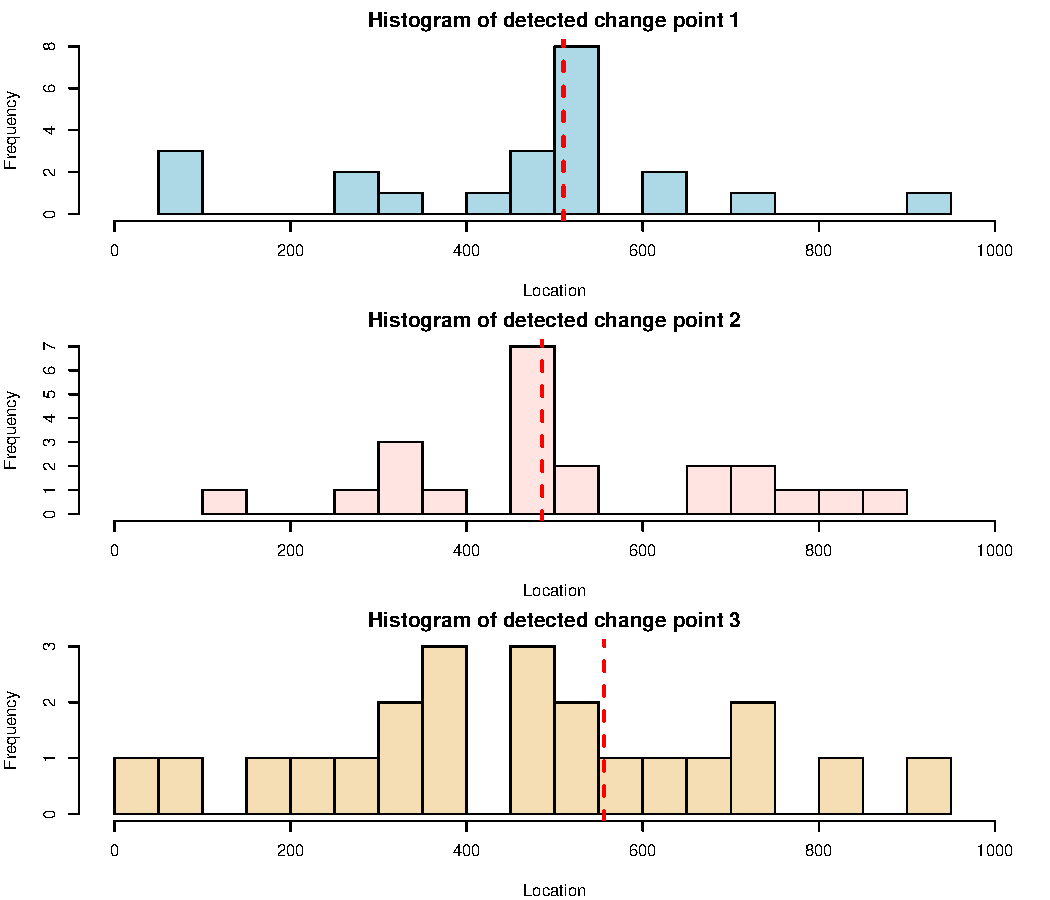
\includegraphics[scale=.45]{images/hist_cps.pdf}
    \caption{Histogram of detected change points for all constructed intervals.}
    \label{fig:1}
\end{figure}


The second task for this application is to partition the subjects into different clusters. In Table \ref{tab:9}, we illustrate the number of estimated groups and the subjects in each group for different partitioned intervals. 
\begin{table}[H]
    \centering
    \caption{Clustered groups for each change point.}
    \label{tab:9}
    \resizebox{\textwidth}{!}{
    \begin{tabular}{c|c|c}
    \hline\hline
        No. of CP & \# clusters & Subjects \\
    \hline
        1 & 4 & (1, 2, 7, 9, 11, 20, 22), (3, 6, 8, 12, 14, 15, 16, 17, 18, 19, 21), (4, 10), (5, 13) \\
        2 & 2 & (1, 2, 3, 4, 5, 6, 7, 8, 10, 12, 13, 14, 15, 16, 17, 18, 19, 20, 21, 22), (9, 11) \\
        3 & 3 & (1, 2, 3, 4, 8, 10, 11, 12, 14, 15, 16, 17, 18, 19, 21, 22), (5, 6, 13), (7, 9, 20) \\
    \hline\hline
    \end{tabular}}
\end{table}

According to Table \ref{tab:9}, one can see that all subjects are not located in the experimental design change point, which is located in the middle. Based on our proposed iterative clustering algorithm (ICA), we find that the first and third change points have more subjects \emph{abnormal} than the second. Our algorithm detects four groups for the first change point, while for the second and third change point, it detects two and three groups respectively. We provide the detailed mean and standard deviation of the individual change points estimated for each group in Table \ref{tab:10}.
\begin{table}[H]
    \centering
    \caption{Mean and standard deviation for each cluster of estimated change points.}
    \label{tab:10}
    \begin{tabular}{c|c|c|c}
    \hline\hline
         & No. Clusters & Mean & Std \\
    \hline
        \multirow{4}*{Change point 1} & 1 & 0.3414 & 0.0569 \\
                                  & 2 & 0.5252 & 0.0315 \\
                                  & 3 & 0.6610 & 0.0113 \\
                                  & 4 & 0.2320 & 0.0028 \\
                                  \hline
        \multirow{2}{*}{Change point 2} & 1 & 0.4815 & 0.0676 \\
                                    & 2 & 0.7505 & 0.0389 \\
                                  \hline
        \multirow{3}{*}{Change point 3} & 1 & 0.5639 & 0.0758 \\
                                    & 2 & 0.3963 & 0.0080 \\
                                    & 3 & 0.2133 & 0.0197 \\
    \hline\hline
    \end{tabular}
\end{table}

From Table \ref{tab:10}, one can see that the estimated change points in the first change point, the mean of estimated change point varies among these four clusters. 

The estimated networks for three different change point segments are presented in the following Figure \ref{fig:2}, \ref{fig:3} and \ref{fig:4}, respectively. In order to present explicitly, we take the average over all individuals in each cluster and only preserve the edges whose value is larger than the pre-determined threshold. 
\begin{figure}[!ht]
    \centering
    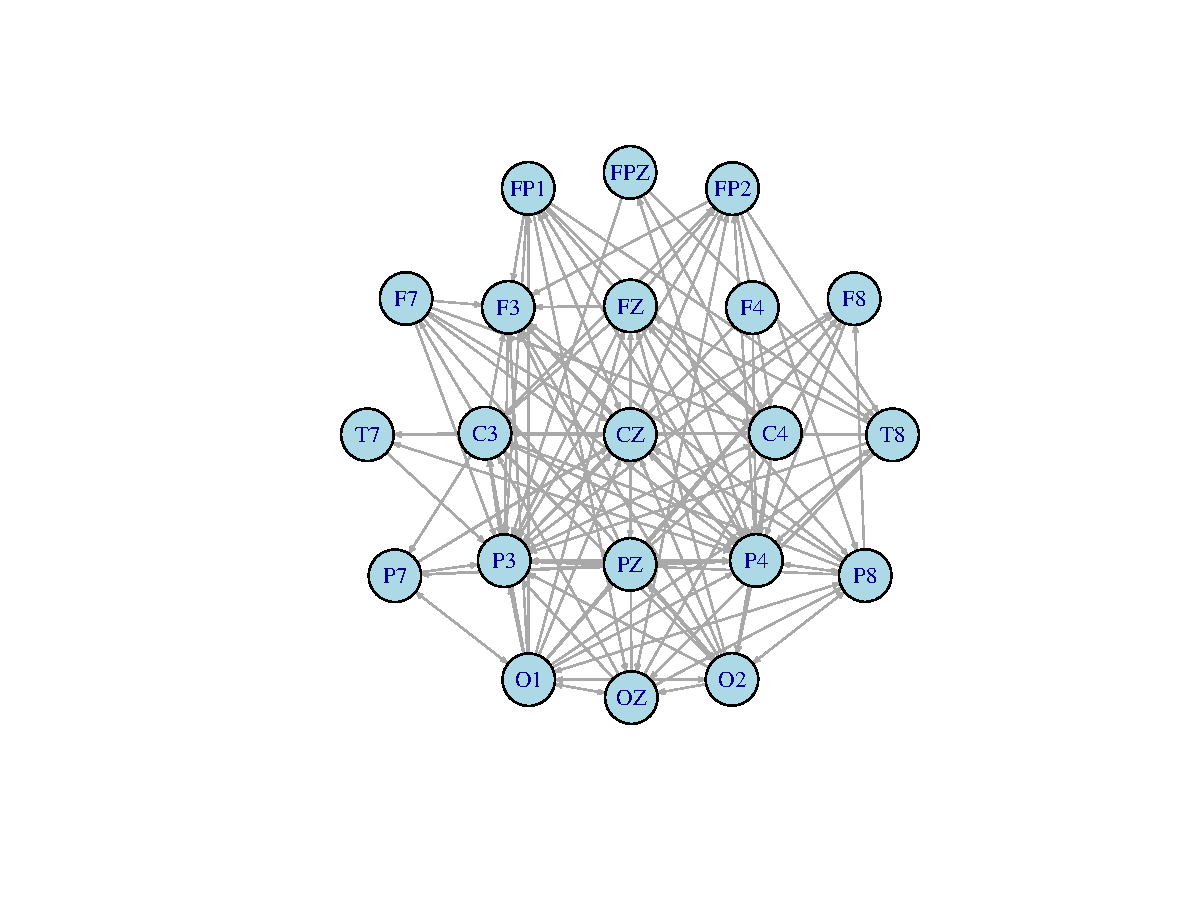
\includegraphics[scale=.22, trim={1.5cm 0.5cm 1.5cm 2cm}, clip]{images/cp1_cluster1_left.pdf}%
    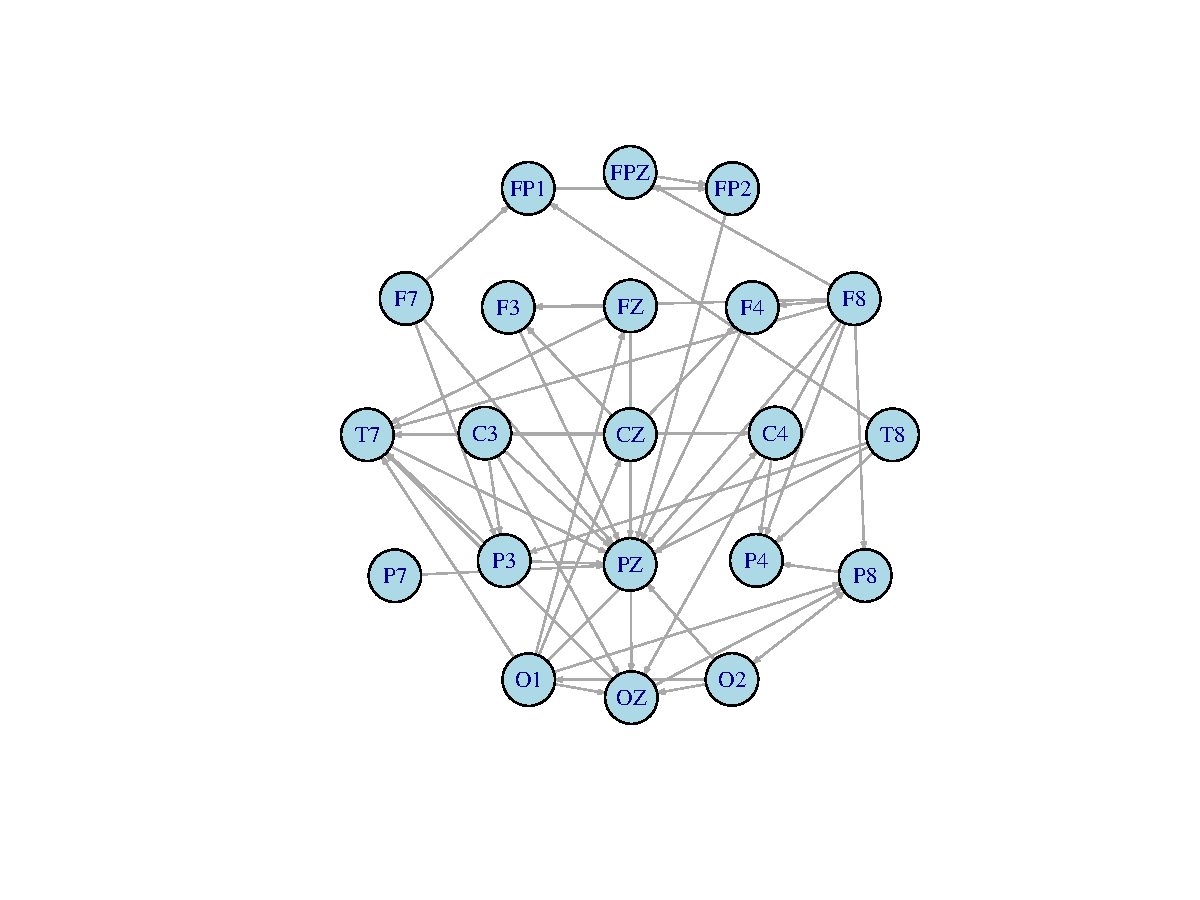
\includegraphics[scale=.22, trim={1.5cm 0.5cm 1.5cm 2cm}, clip]{images/cp1_cluster2_left.pdf}%
    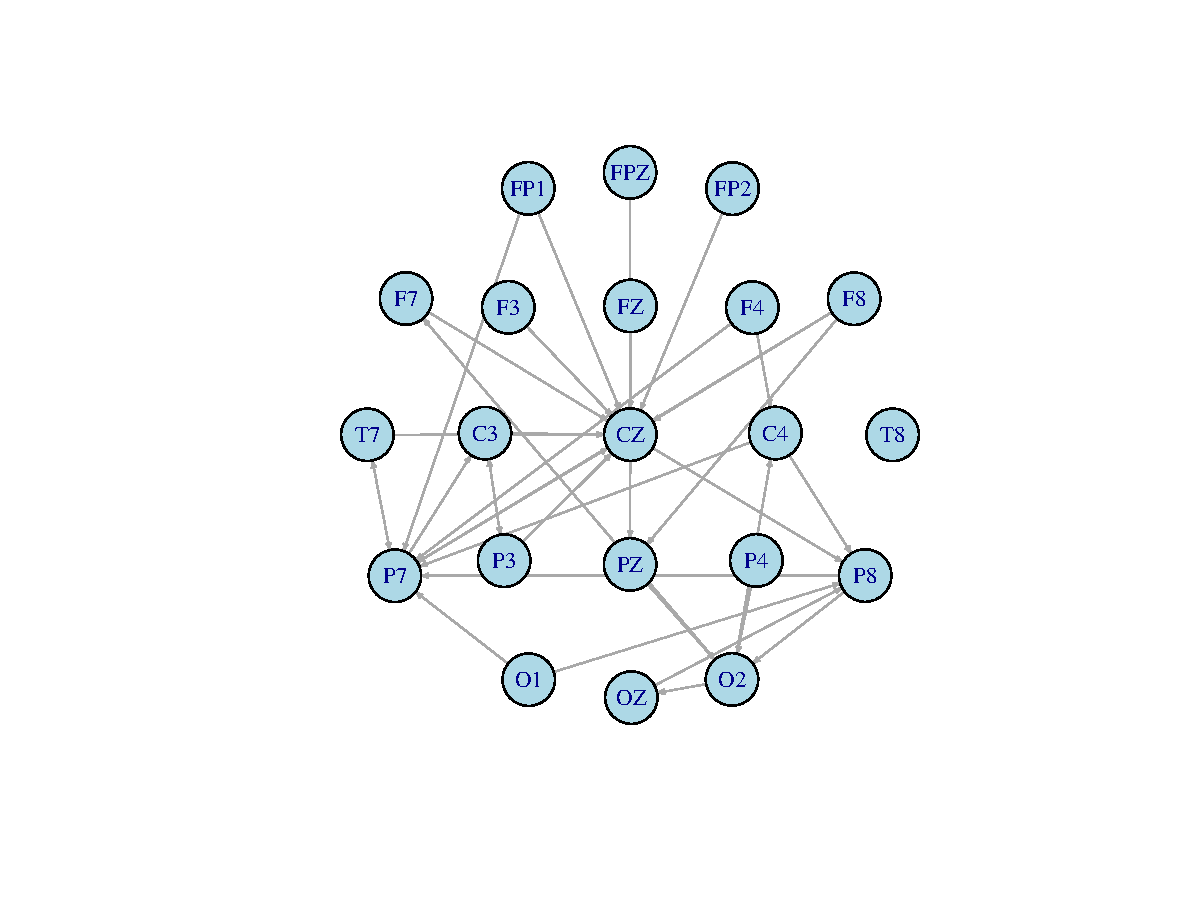
\includegraphics[scale=.22, trim={1.5cm 0.5cm 1.5cm 2cm}, clip]{images/cp1_cluster3_left.pdf}%
    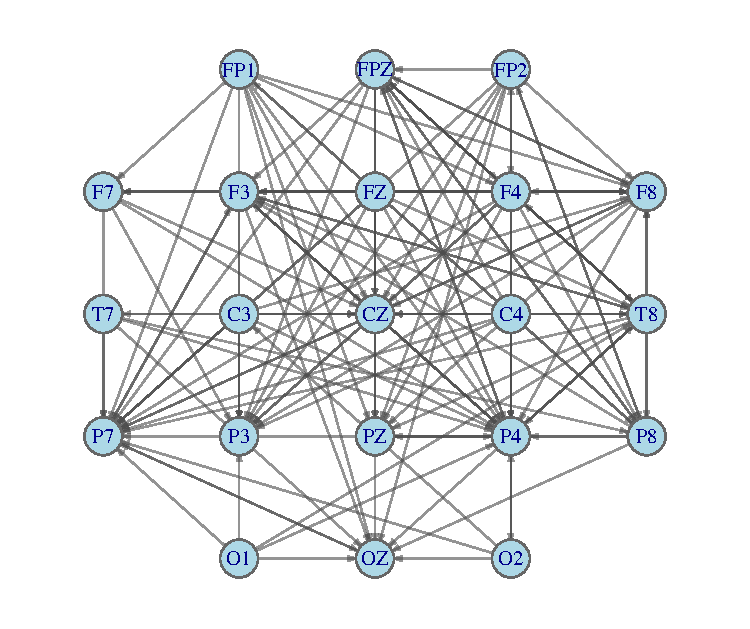
\includegraphics[scale=.22, trim={1.5cm 0.5cm 1.5cm 2cm}, clip]{images/cp1_cluster4_left.pdf}%
    \vfill
    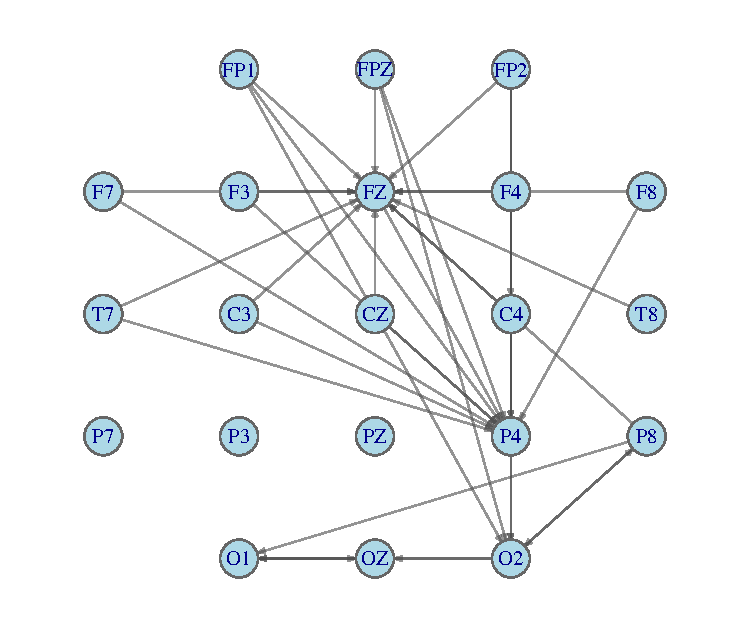
\includegraphics[scale=.22, trim={1.5cm 0.5cm 1.5cm 2cm}, clip]{images/cp1_cluster1_right.pdf}%
    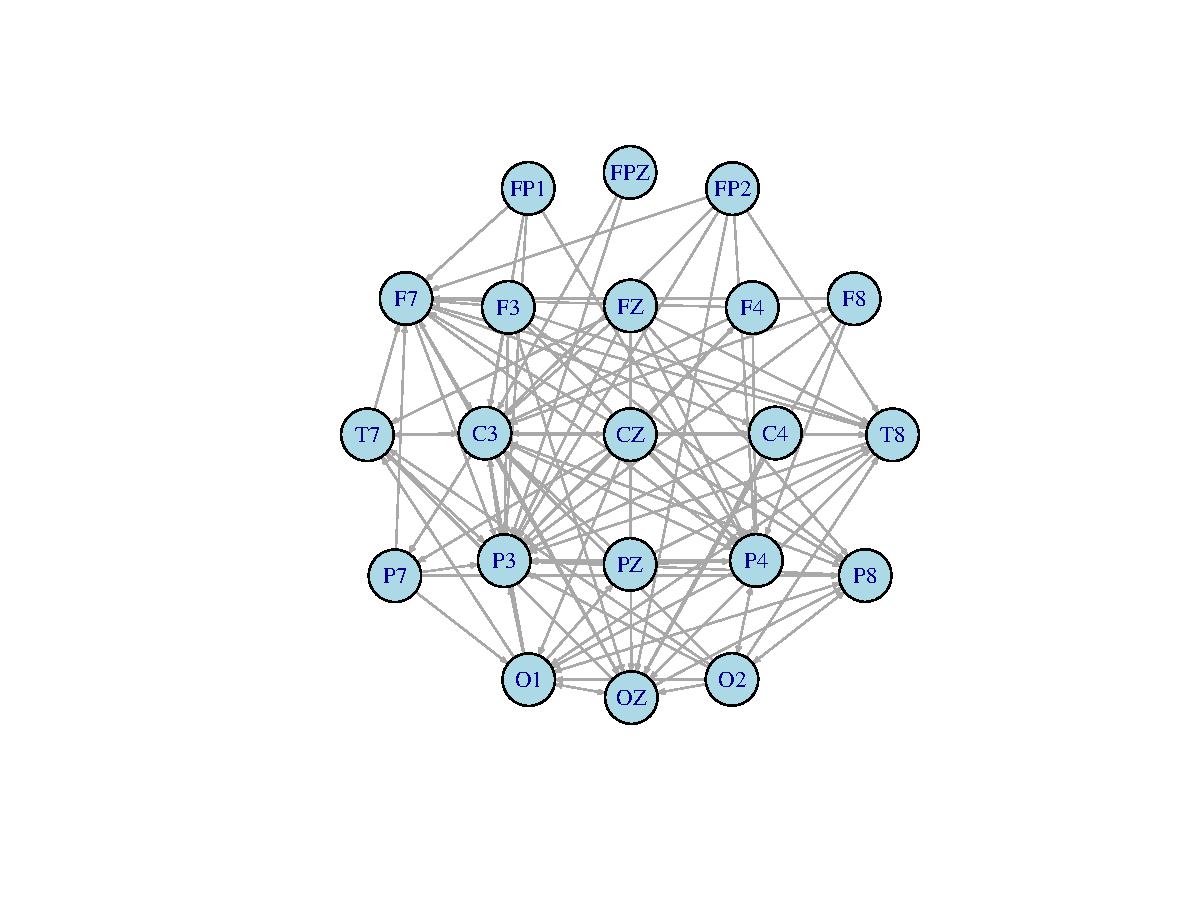
\includegraphics[scale=.22, trim={1.5cm 0.5cm 1.5cm 2cm}, clip]{images/cp1_cluster2_right.pdf}%
    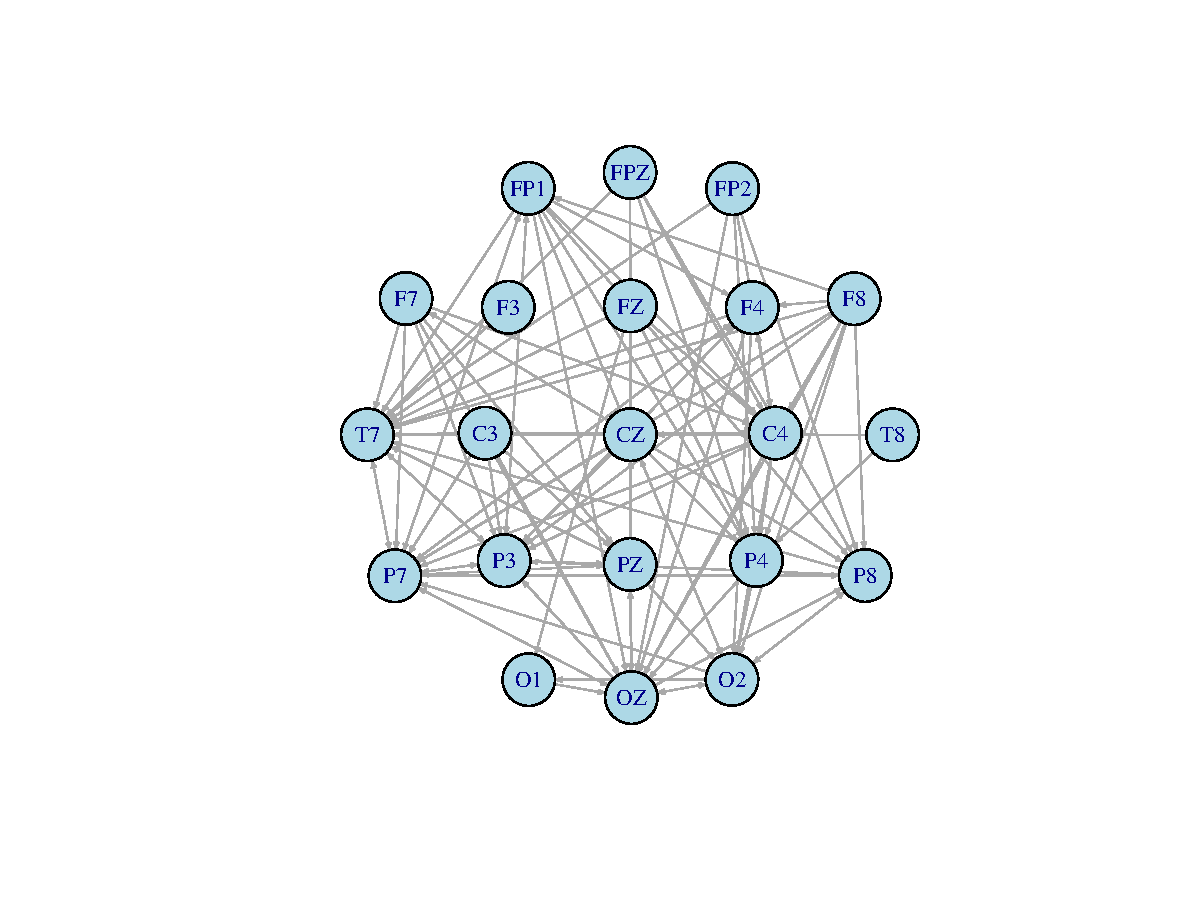
\includegraphics[scale=.22, trim={1.5cm 0.5cm 1.5cm 2cm}, clip]{images/cp1_cluster3_right.pdf}%
    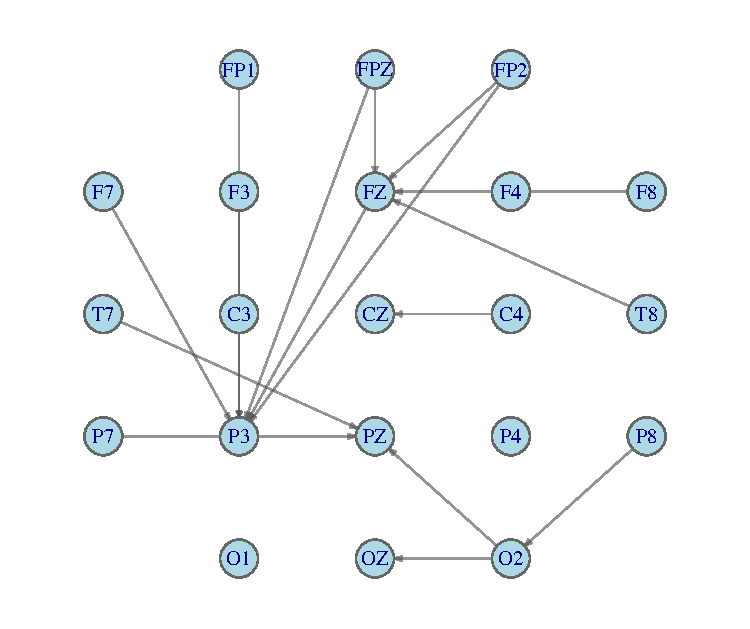
\includegraphics[scale=.22, trim={1.5cm 0.5cm 1.5cm 2cm}, clip]{images/cp1_cluster4_right.pdf}
    \caption{The averaged estimated networks for the different clusters for the first interval. Top row: the networks for the left part of estimated individual change points; Bottom row: the networks for the right part of estimated individual change points.}
    \label{fig:2}
\end{figure}

\begin{figure}[!ht]
    \centering
    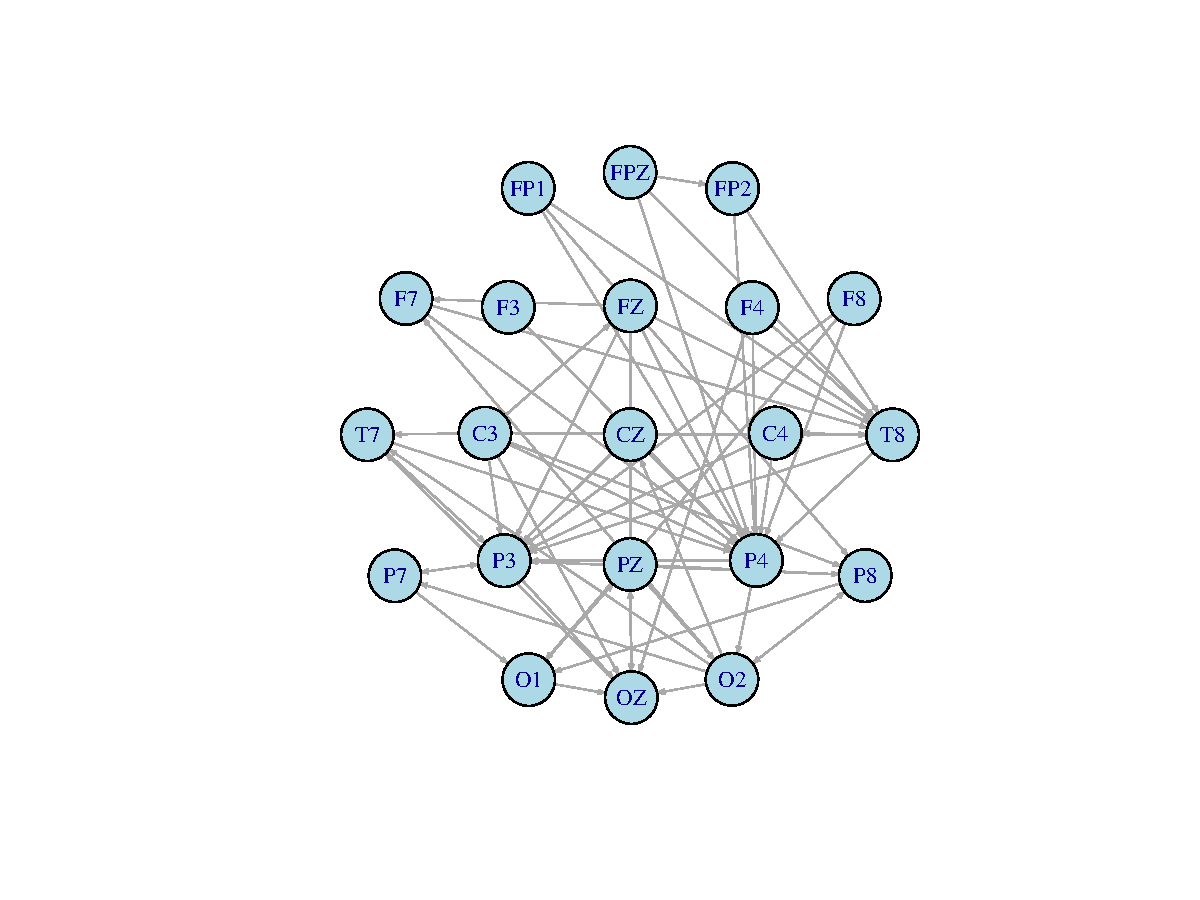
\includegraphics[scale=.22, trim={1.5cm 0.5cm 1.5cm 2cm}, clip]{images/cp2_cluster1_left.pdf}%
    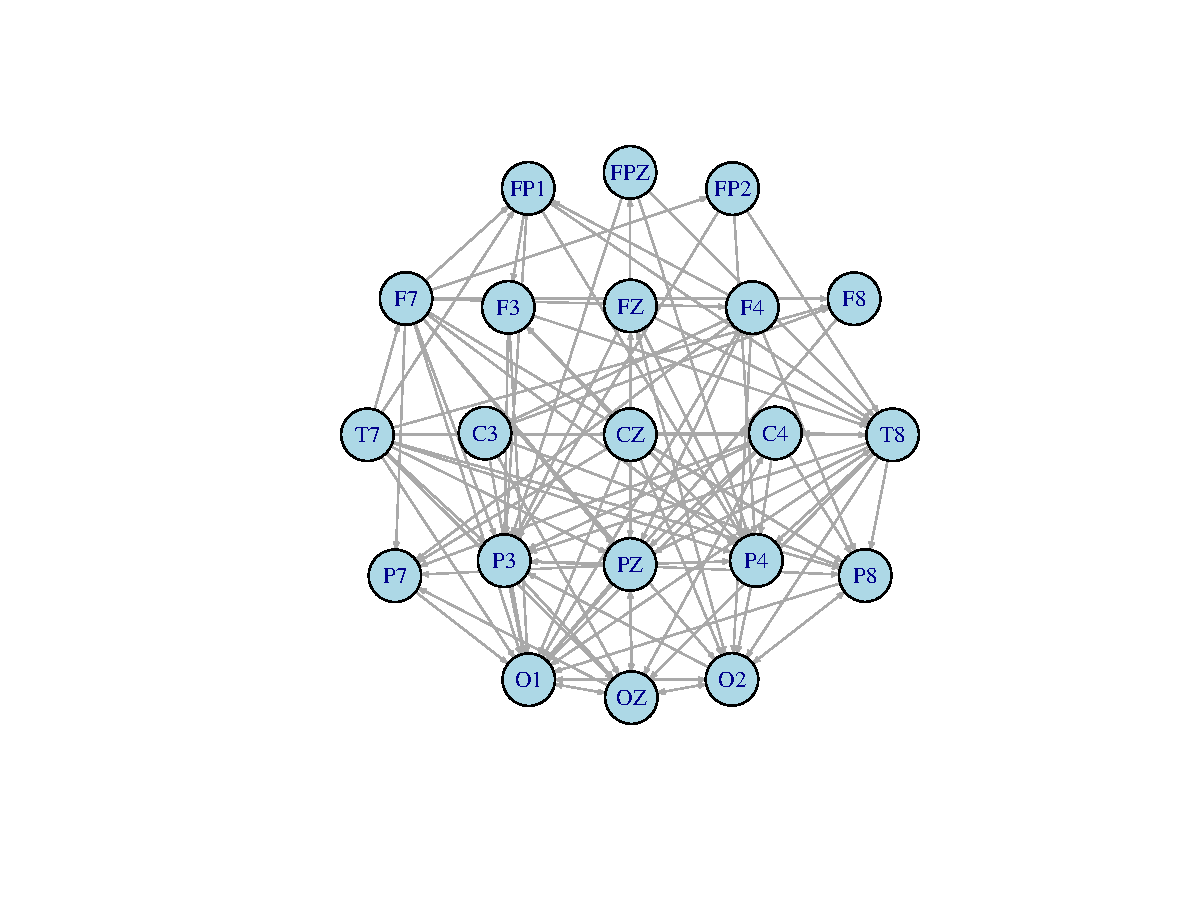
\includegraphics[scale=.22, trim={1.5cm 0.5cm 1.5cm 2cm}, clip]{images/cp2_cluster2_left.pdf}%
    \vfill
    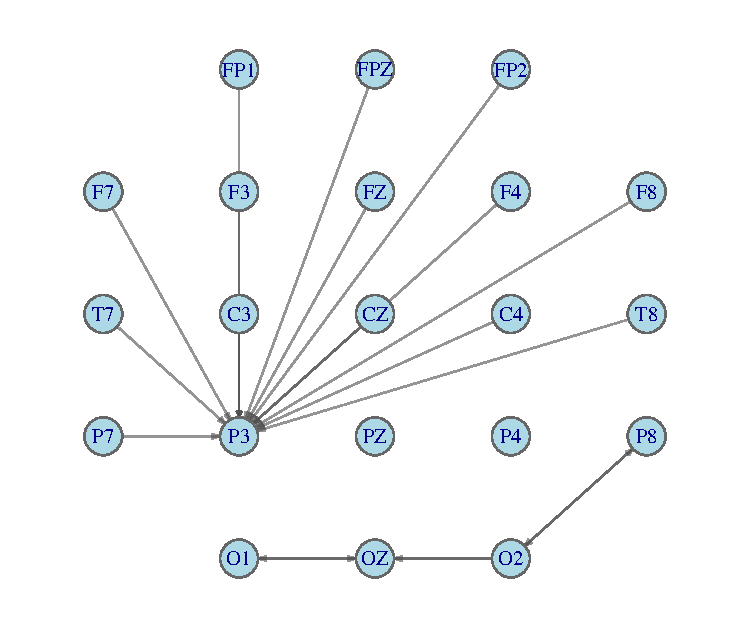
\includegraphics[scale=.22, trim={1.5cm 0.5cm 1.5cm 2cm}, clip]{images/cp2_cluster1_right.pdf}%
    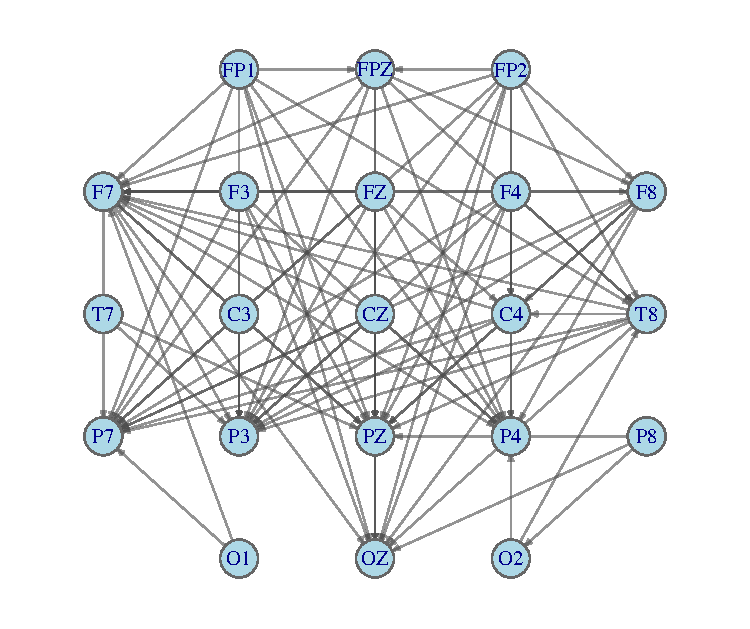
\includegraphics[scale=.22, trim={1.5cm 0.5cm 1.5cm 2cm}, clip]{images/cp2_cluster2_right.pdf}
    \caption{The averaged estimated networks for the different clusters for the second interval. Top row: the networks for the left part of estimated individual change points; Bottom row: the networks for the right part of estimated individual change points.}
    \label{fig:3}
\end{figure}

\begin{figure}[!ht]
    \centering
    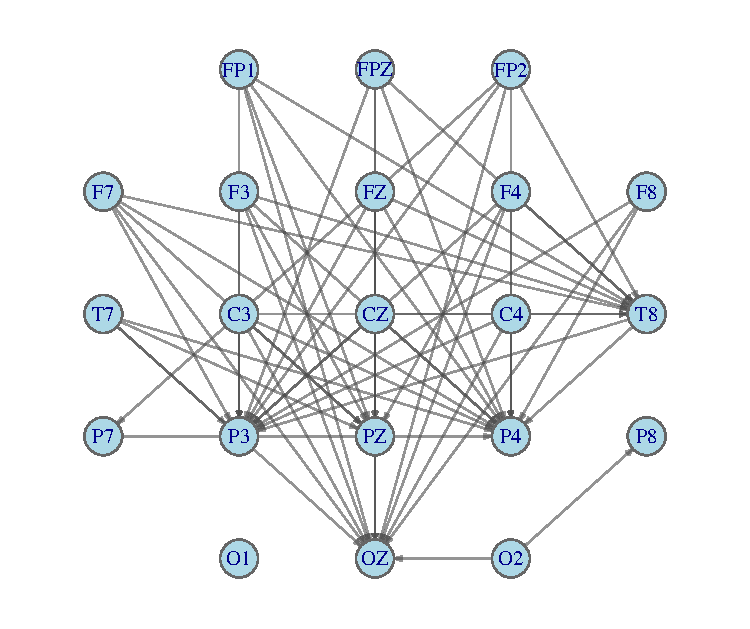
\includegraphics[scale=.22, trim={1.5cm 0.5cm 1.5cm 2cm}, clip]{images/cp3_cluster1_left.pdf}%
    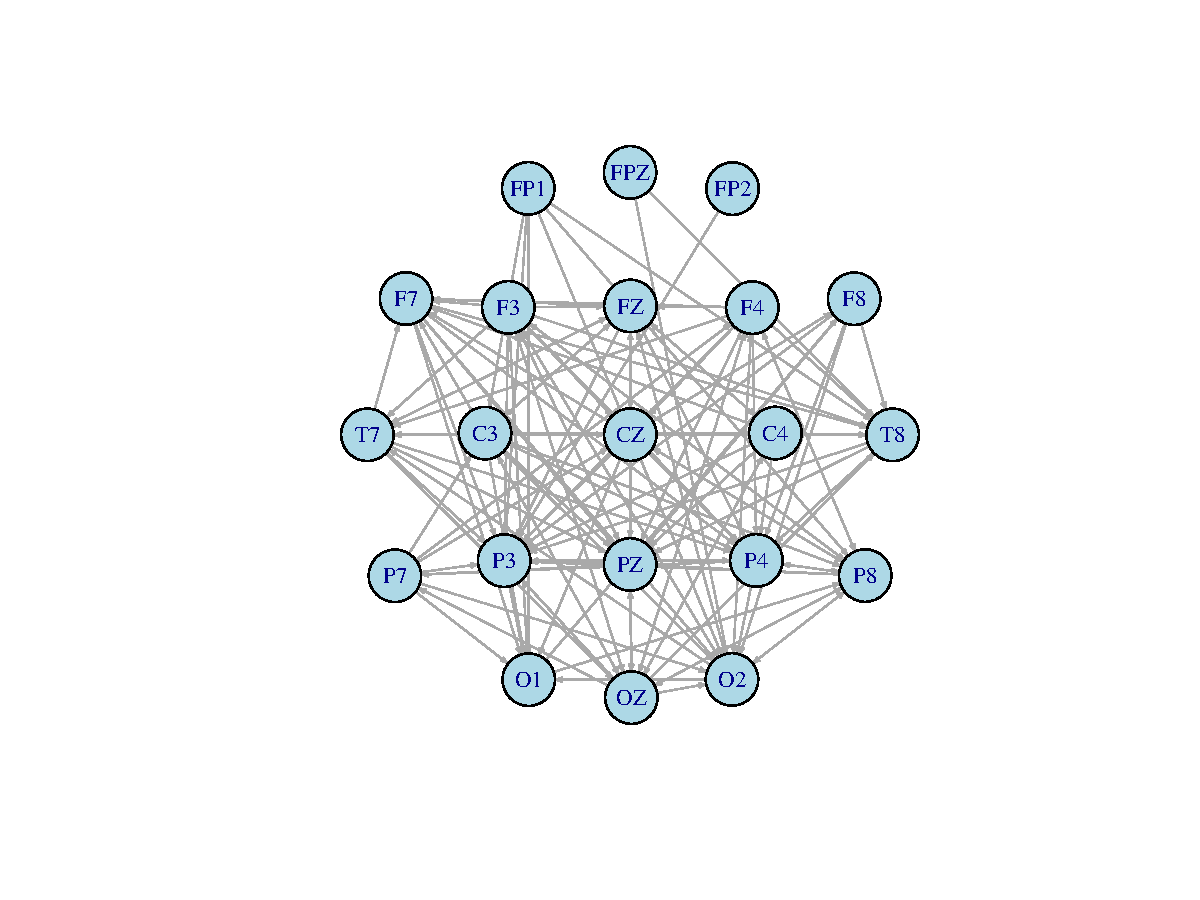
\includegraphics[scale=.22, trim={1.5cm 0.5cm 1.5cm 2cm}, clip]{images/cp3_cluster2_left.pdf}%
    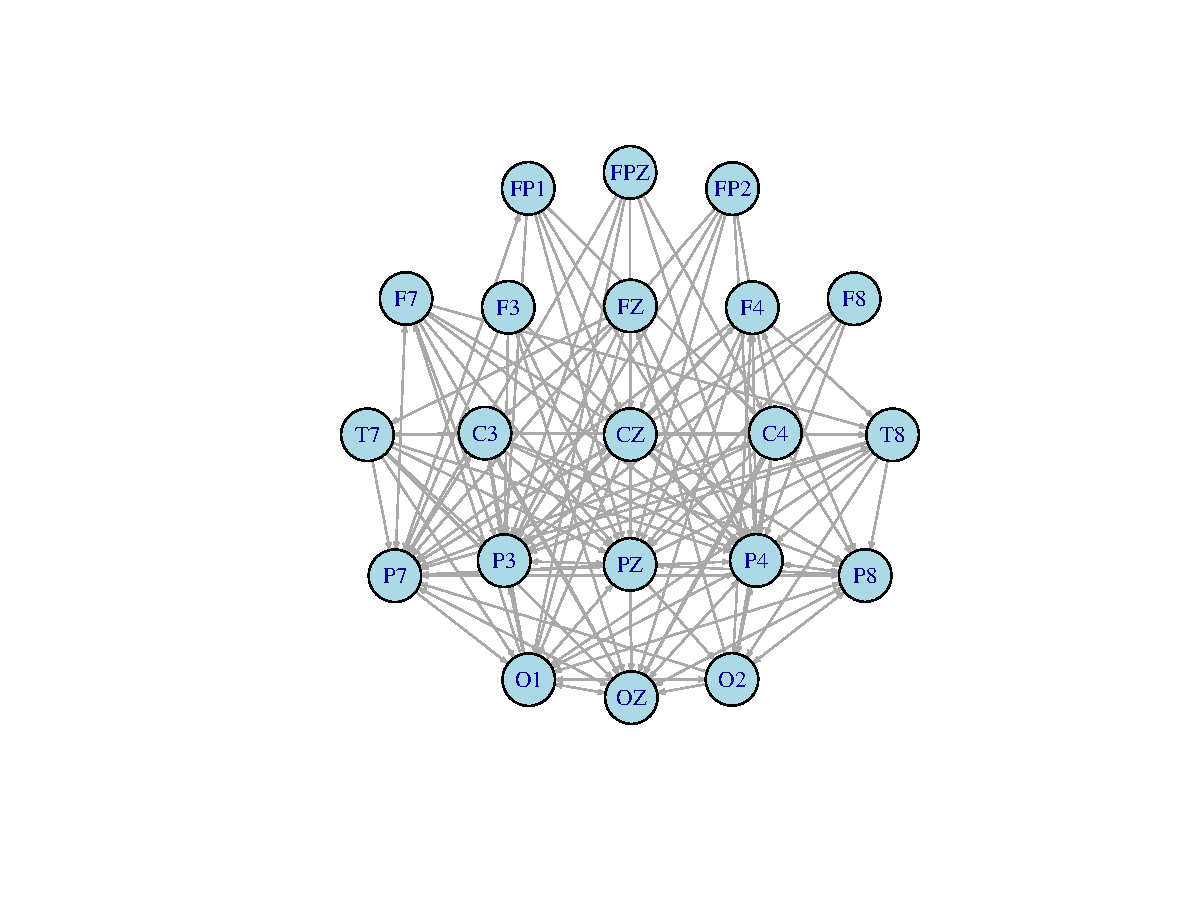
\includegraphics[scale=.22, trim={1.5cm 0.5cm 1.5cm 2cm}, clip]{images/cp3_cluster3_left.pdf}%
    \vfill
    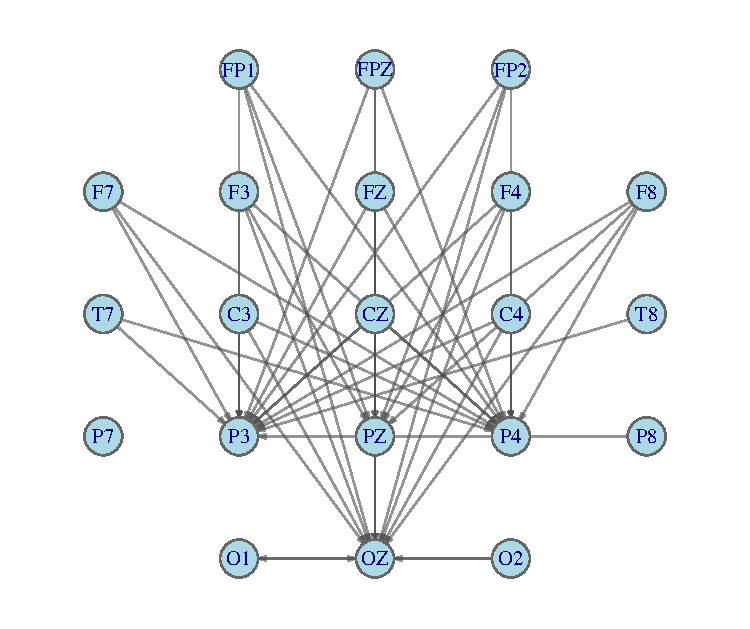
\includegraphics[scale=.22, trim={1.5cm 0.5cm 1.5cm 2cm}, clip]{images/cp3_cluster1_right.pdf}%
    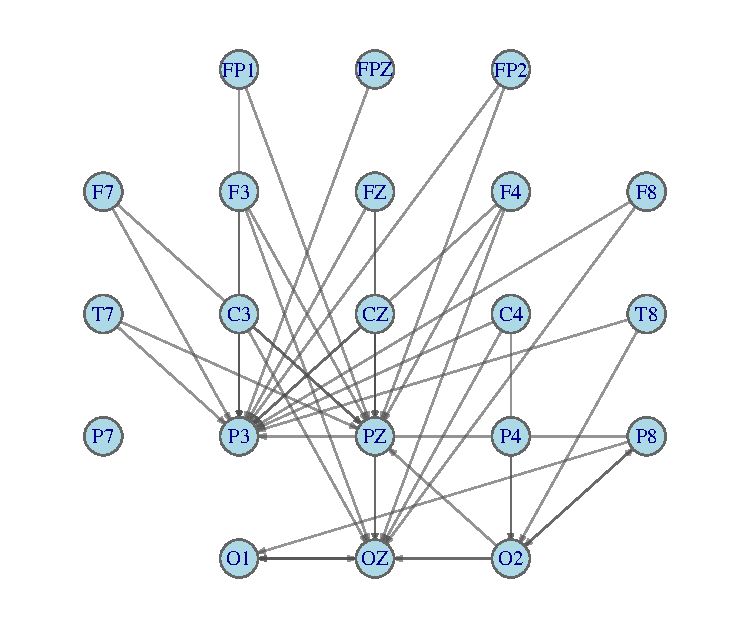
\includegraphics[scale=.22, trim={1.5cm 0.5cm 1.5cm 2cm}, clip]{images/cp3_cluster2_right.pdf}%
    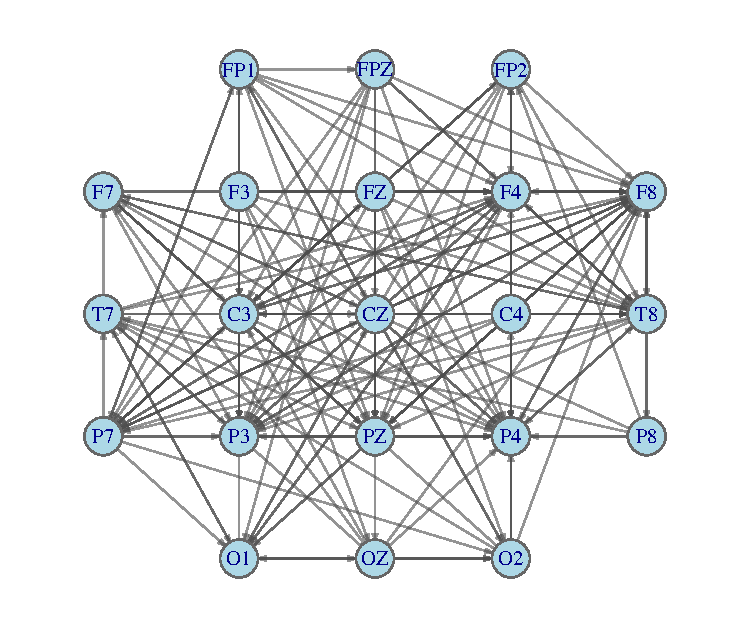
\includegraphics[scale=.22, trim={1.5cm 0.5cm 1.5cm 2cm}, clip]{images/cp3_cluster3_right.pdf}%
    \caption{The averaged estimated networks for the different clusters for the third interval. Top row: the networks for the left part of estimated individual change points; Bottom row: the networks for the right part of estimated individual change points.}
    \label{fig:4}
\end{figure}

According to the estimated networks, we can see that the density of the network pairs differs across clusters, and the dominant within-cluster connections are concentrated on a small subset of channels, suggesting that the same experimental transition is reflected in subject-specific functional connectivity patterns rather than a single shared network.

We also provide the Hamming distance among detected clusters within each interval.
\begin{figure}[!ht]
    \centering
    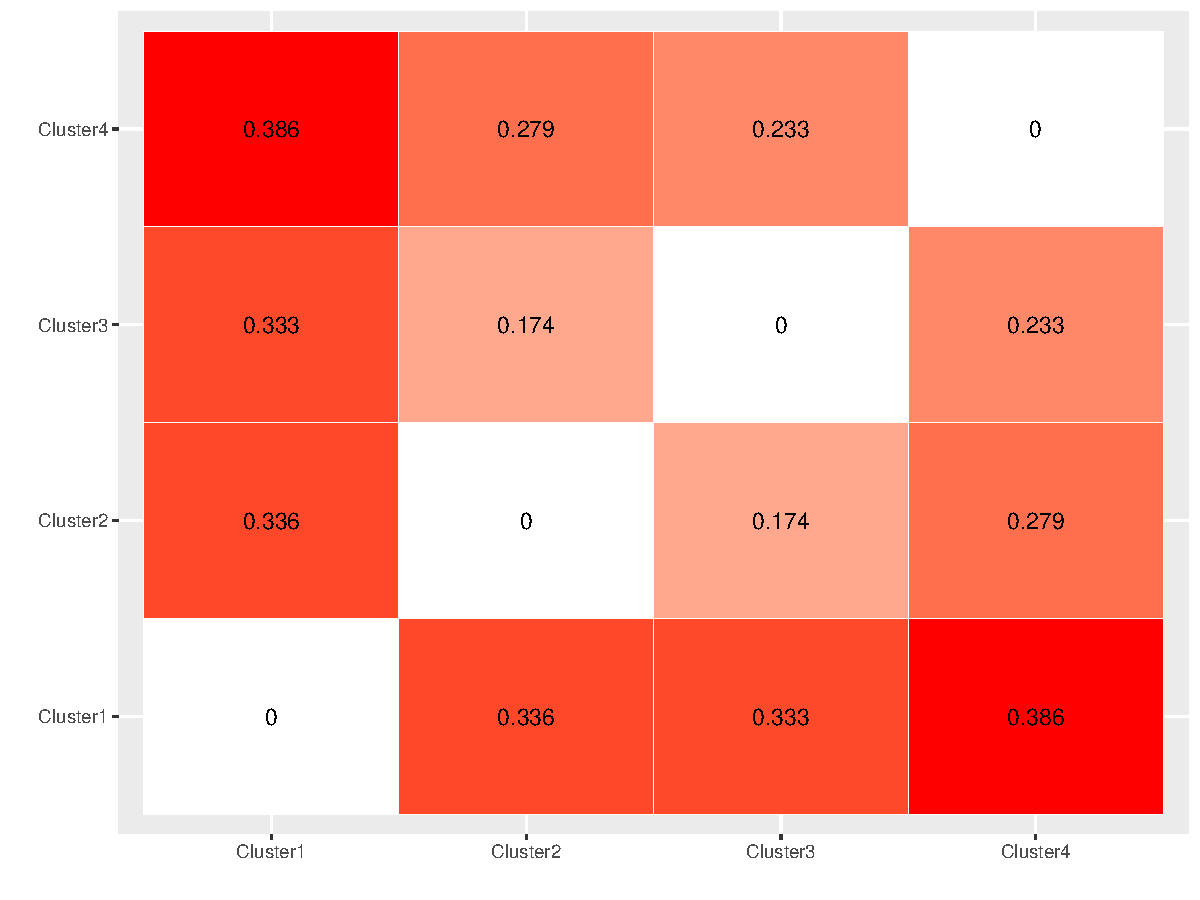
\includegraphics[scale=.24]{images/cp1_left_hamming.pdf}%
    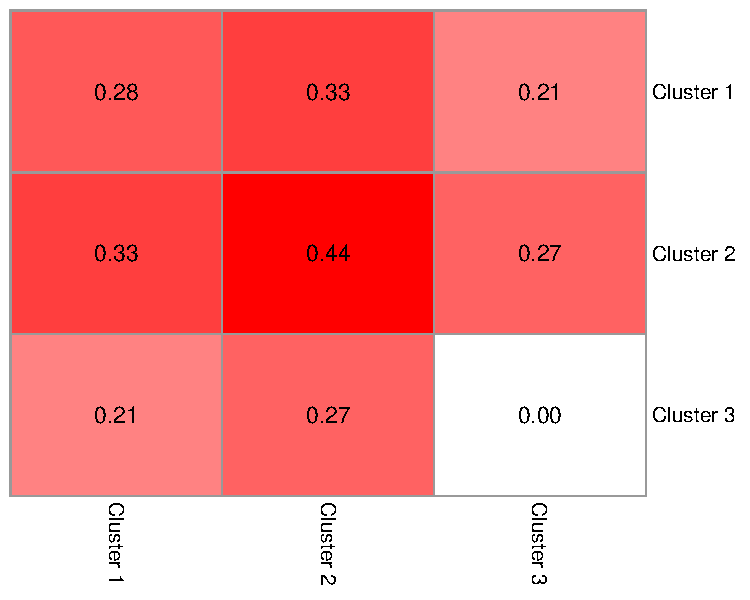
\includegraphics[scale=.24]{images/cp2_left_hamming.pdf}%
    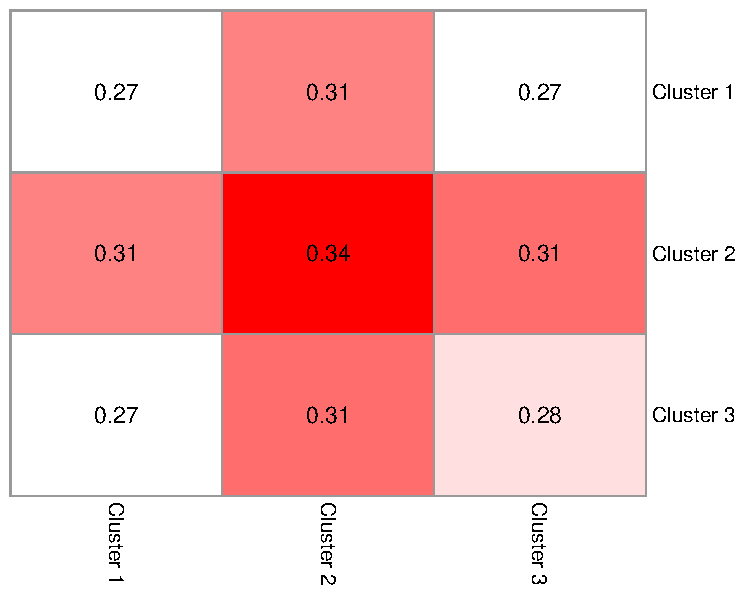
\includegraphics[scale=.24]{images/cp3_left_hamming.pdf}%
    \vfill
    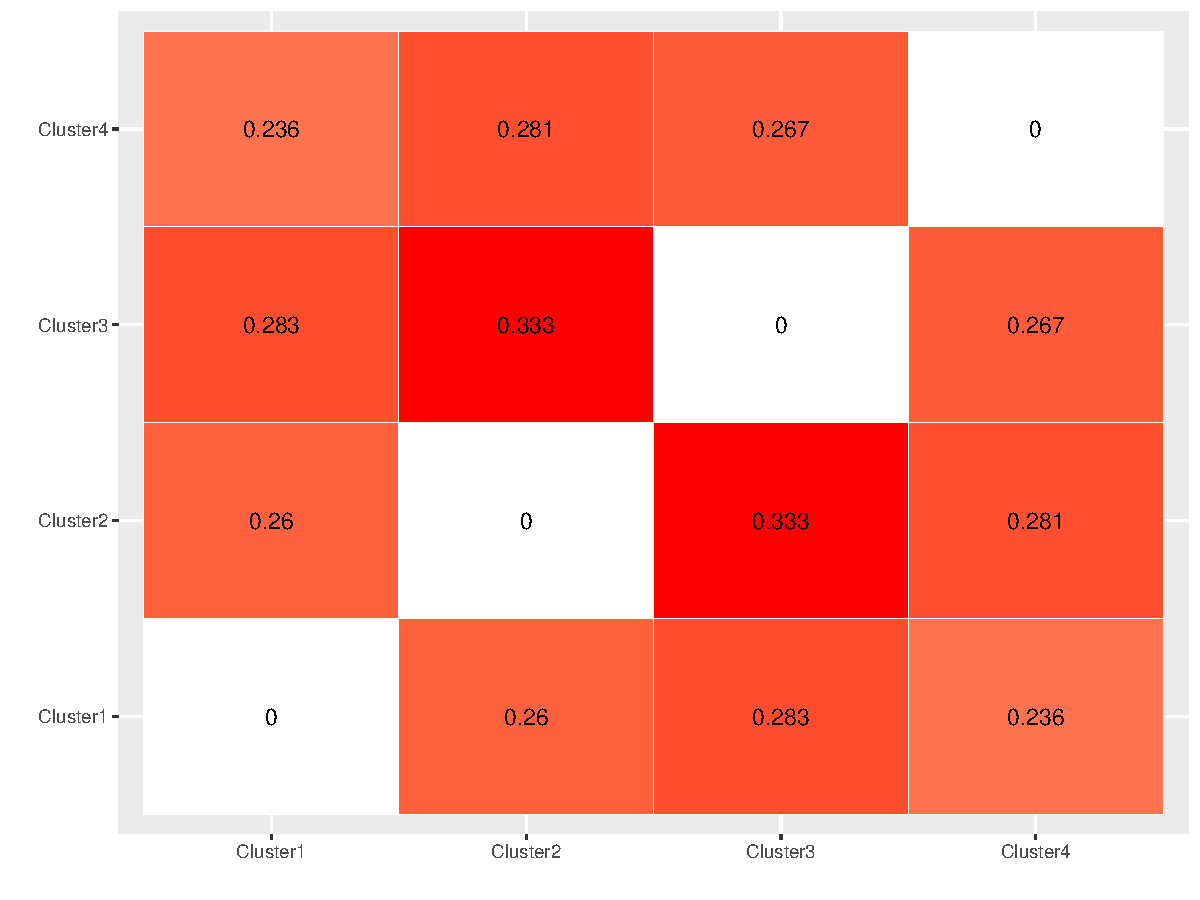
\includegraphics[scale=.24]{images/cp1_right_hamming.pdf}%
    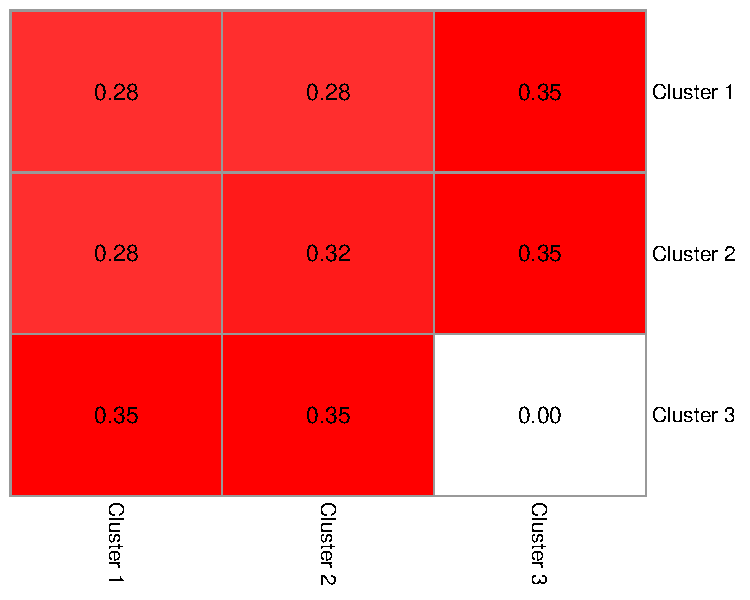
\includegraphics[scale=.24]{images/cp2_right_hamming.pdf}%
    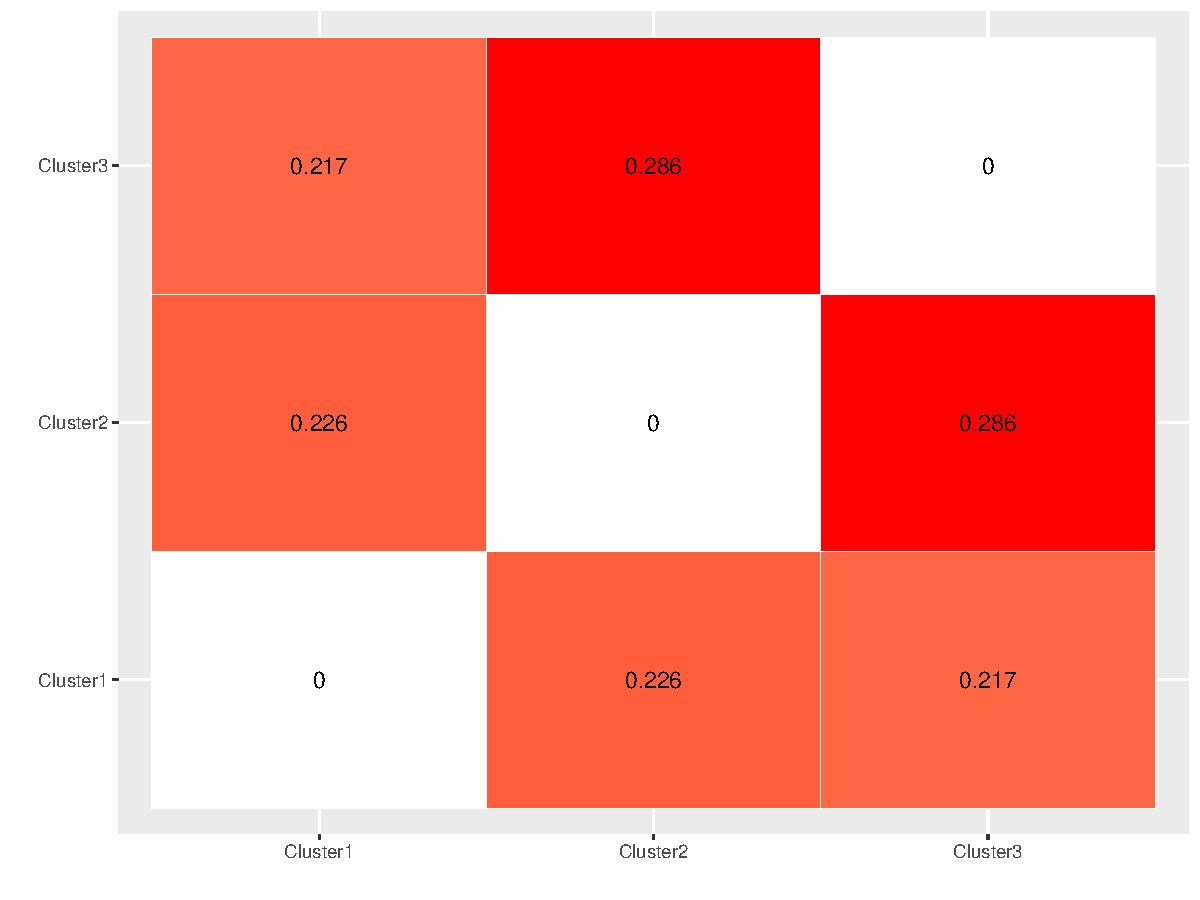
\includegraphics[scale=.24]{images/cp3_right_hamming.pdf}
    \caption{Hamming distance of estimated networks among different clusters for each interval. Top row: hamming distance matrices for the estimated networks for the left-hand side of detected individual change points; Bottom row: hamming distance matrices for the estimated networks for the right-hand side of detected individual change points.}
    \label{fig:5}
\end{figure}

\subsection{More conservative results}
Here we use a more conservative setting to cluster the change points for each interval. 
\begin{table}[!ht]
    \centering
    \caption{Clustered groups for each change point.}
    \label{tab:11}
    \resizebox{\textwidth}{!}{
    \begin{tabular}{c|c|c}
    \hline\hline
        No. of CP & \# clusters & Subjects \\
    \hline
        1 & 3 & (1, 2, 3, 5, 7, 9, 11, 20, 22), (4, 6, 8, 10, 12, 14, 15, 16, 17, 18, 19, 21), (13) \\
        2 & 2 & (1, 2, 3, 4, 5, 6, 7, 8, 10, 12, 13, 14, 15, 16, 17, 18, 19, 20, 21, 22), (9, 11) \\
        3 & 2 & (1, 2, 3, 4, 5, 6, 8, 10, 11, 12, 13, 14, 15, 16, 17, 18, 19, 21, 22), (7, 9, 20) \\
    \hline\hline
    \end{tabular}}
\end{table}

For the first change point interval, one can see that we have two clusters with more than 5 individuals, hence, in order to illustrate the difference between these individuals, we present the box plot for their ages in the following Figure \ref{fig:6}. 
\begin{figure}[!ht]
    \centering
    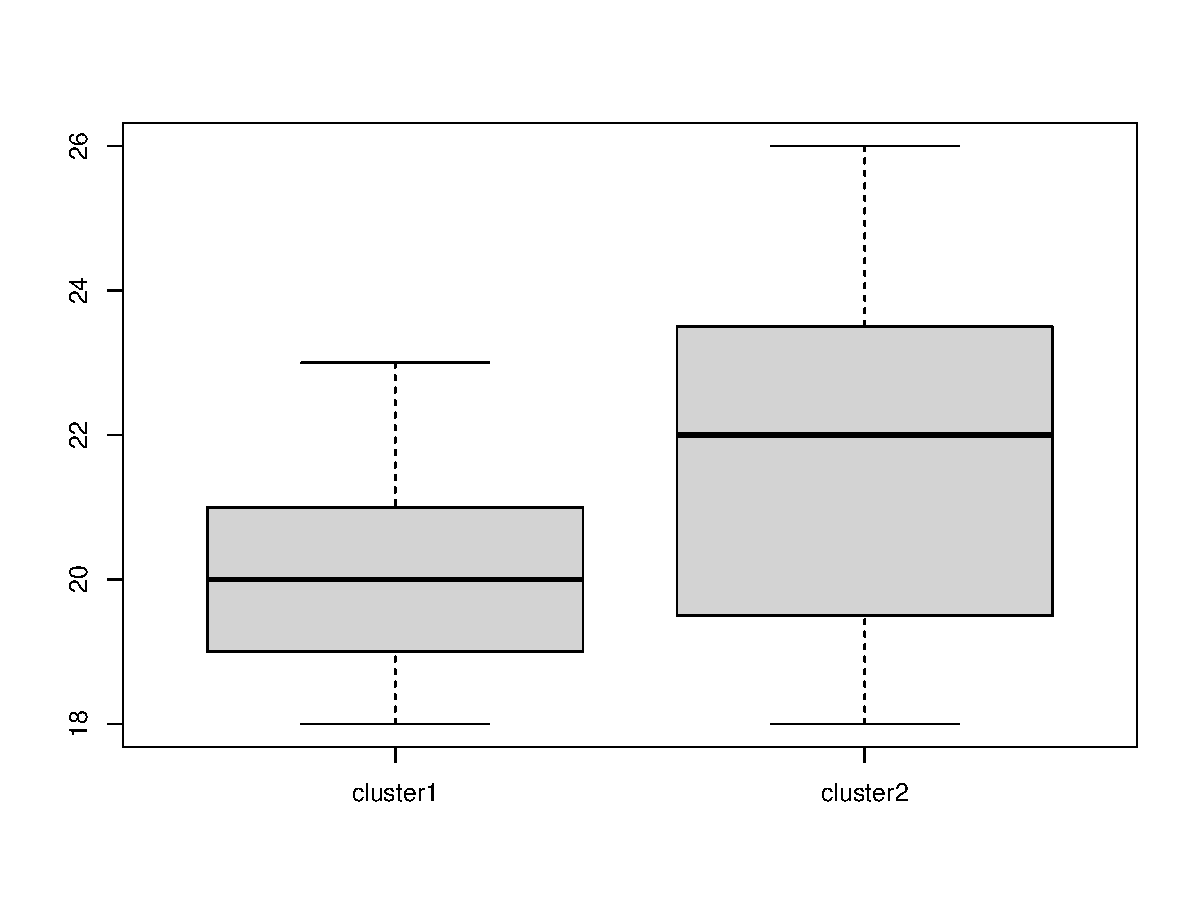
\includegraphics[scale=.4]{images/age_group_boxplots.pdf}
    \caption{Box-plot for the age of the individuals in the first two clusters in the first change point interval.}
    \label{fig:6}
\end{figure}

Specifically, there are 9 and 12 individuals in these two clusters respectively, and the mean ages of these two clusters are 20.33 and 21.83.
Since there are no samples, we apply the permutation t-test to examine the significance of the difference. The $t$-statistics are -1.5154, and the corresponding $p$-value is 0.1459. 

\subsection{Other results}
We present its series and detected change point to investigate the pattern and behavior in subject 13 using the within/between clusters hamming distances. 

\begin{figure}[!ht]
    \centering
    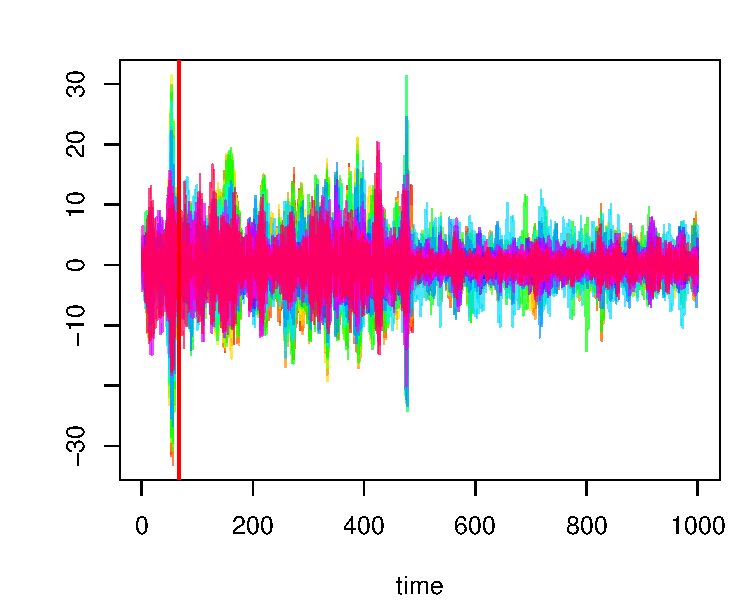
\includegraphics[scale=.4]{images/subject_13.pdf}%
    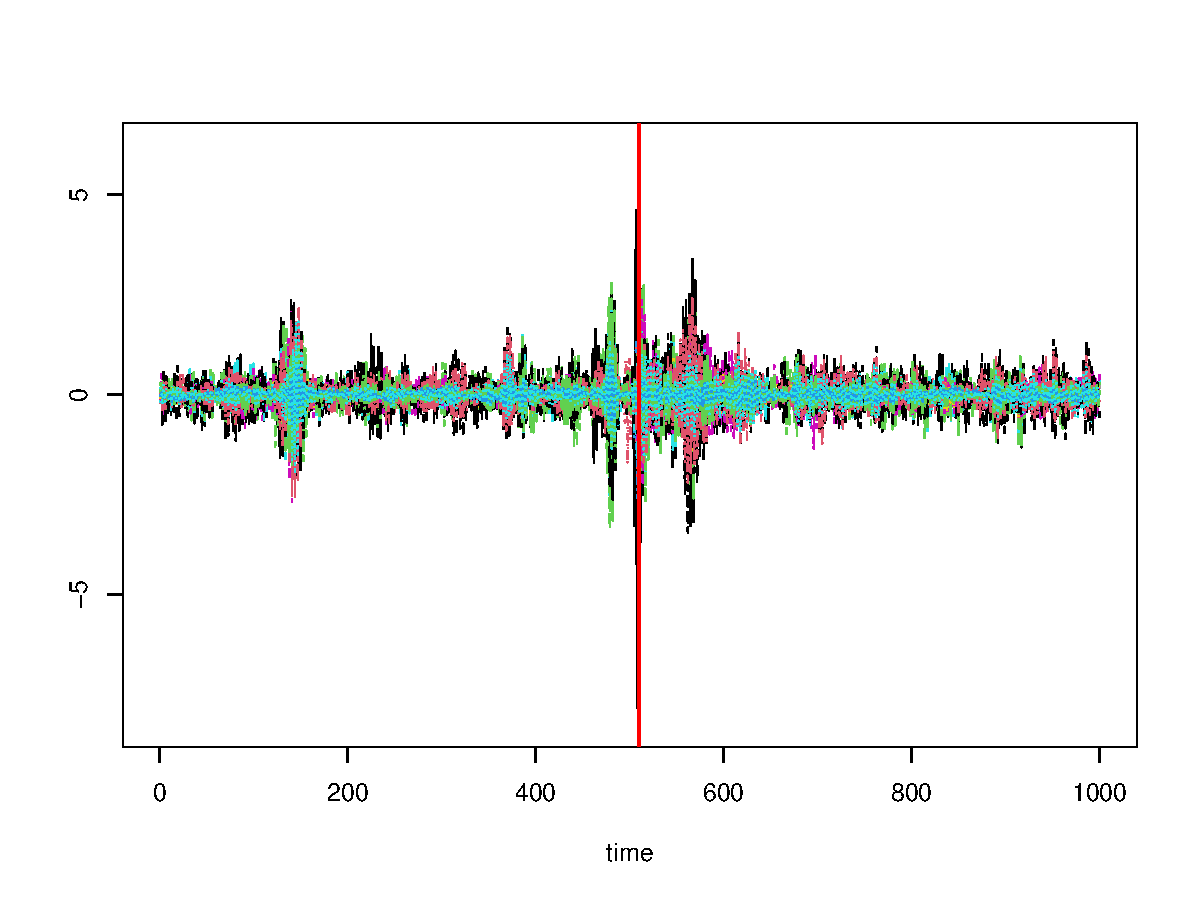
\includegraphics[scale=.4]{images/subject_6.pdf}
    \caption{Left panel: subject 13 (outlier) and its detected change point $\hat{t}=230$; Right panel: a \emph{normal} example of subject and its change point $\hat{t} = 510$.}
    \label{fig:7}
\end{figure}

For the within/between clusters Hamming distances, we have the following table to present all results. In the first table, we present the averaged Hamming distances over all subjects' estimated networks within/between different clusters for the clustered groups with mild clustering threshold presented in Table \ref{tab:9}. 
\begin{table}[!ht]
    \centering
    \caption{The averaged within/between Hamming distances over all subjects in different clusters. (1st change point)}
    \label{tab:wb-dist-cp1}
    \begin{tabular}{c|c|c|c|c}
    \hline\hline
         & Cluster 1 & Cluster 2 & Cluster 3 & Cluster 4 \\
    \hline
         Cluster 1 & 0.227 & 0.274 & 0.270 & \textcolor{red}{0.352} \\
         Cluster 2 & - & 0.252 & 0.275 & \textcolor{red}{0.377} \\
         Cluster 3 & - & - & 0.145 & \textcolor{red}{0.366} \\
         Cluster 4 & - & - & - & 0.228 \\
    \hline\hline
    \end{tabular}
\end{table}

\begin{table}[!ht]
    \centering
    \caption{The averaged within/between Hamming distances over all subjects in different clusters. (2nd change point)}
    \label{tab:wb-dist-cp2}
    \begin{tabular}{c|c|c}
    \hline\hline
         & Cluster 1 & Cluster 2 \\
    \hline
         Cluster 1 & 0.266 & \textcolor{red}{0.285} \\
         Cluster 2 & - & 0.126 \\
    \hline\hline
    \end{tabular}
\end{table}

\begin{table}[!ht]
    \centering
    \caption{The averaged within/between Hamming distances over all subjects in different clusters. (3rd change point)}
    \label{tab:wb-dist-cp3}
    \begin{tabular}{c|c|c|c}
    \hline\hline
         & Cluster 1 & Cluster 2 & Cluster 3 \\
    \hline
         Cluster 1 & 0.267 & \textcolor{red}{0.311} & 0.285 \\
         Cluster 2 & - & 0.212 & \textcolor{red}{0.286} \\
         Cluster 3 & - & - & 0.150 \\
    \hline\hline
    \end{tabular}
\end{table}

Similarly, we present the within/between clusters Hamming distances for conservative results.
\begin{table}[!ht]
    \centering
    \caption{The averaged within/between Hamming distances over all subjects in different clusters. (1st change point)}
    \label{tab:wb-dist-cp1-conserve}
    \begin{tabular}{c|c|c|c}
    \hline\hline
         & Cluster 1 & Cluster 2 & Cluster 3 \\
    \hline
         Cluster 1 & 0.299 & \textcolor{red}{0.310} & 0.301 \\
         Cluster 2 & - & 0.271 & \textcolor{red}{0.277} \\
         Cluster 3 & - & - & 0 \\
    \hline\hline
    \end{tabular}
\end{table}
\begin{table}[!ht]
    \centering
    \caption{The averaged within/between Hamming distances over all subjects in different clusters. (2nd change point)}
    \label{tab:wb-dist-cp2-conserve}
    \begin{tabular}{c|c|c}
    \hline\hline
         & Cluster 1 & Cluster 2 \\
    \hline
         Cluster 1 & 0.263 & \textcolor{red}{0.288} \\
         Cluster 2 & - & 0.103 \\
    \hline\hline
    \end{tabular}
\end{table}
\begin{table}[!ht]
    \centering
    \caption{The averaged within/between Hamming distances over all subjects in different clusters. (3rd change point)}
    \label{tab:wb-dist-cp3-conserve}
    \begin{tabular}{c|c|c}
    \hline\hline
         & Cluster 1 & Cluster 2 \\
    \hline
         Cluster 1 & 0.269 & \textcolor{red}{0.290} \\
         Cluster 2 & - & 0.150 \\
    \hline\hline
    \end{tabular}
\end{table}

\section{Concluding Remarks}\label{sec:conclude}
We introduced a unified framework for detecting change points in a cohort of high-dimensional sparse VAR time series, in which each subject's break locations lie within a ball of radius $r_T$ around an unknown cohort centre. The framework comprises a single-change-point cohort estimator with both a maximum-lag and a minimum-lag detection strategy (Theorems \ref{thm:1} and \ref{thm:1b}); a multi-change-point procedure that combines a rolling-window scan, a localized information criterion, and a cluster-level exhaustive search (Theorems \ref{thm:2}--\ref{thm:3}); and an iterative clustering algorithm that recovers group structure when the cohort assumption is violated for a subset of subjects. The non-asymptotic error bounds match the rate of \cite{wang2019localizing} once $r_T$ is comparable to $s_{\max}\log p$.

Across twelve simulation scenarios that vary the dimension, sample size, number of subjects, jump structure, and noise distribution, the cohort estimators recover the change points with relative bias below $0.01$ and standard deviation roughly one order of magnitude smaller than per-subject baselines. On a shared evaluation setting (scenario G4) the proposed method outperforms sparsified binary segmentation, binary segmentation, and the factor-adjusted VAR segmentation procedure of \cite{cho2023high} on every metric reported. On the EEG cohort of \cite{trujillo2017effect} the iterative clustering algorithm separates participants into interpretable groups around each of the three experimental transitions, and the within- versus between-cluster Hamming distances of the estimated network structures are consistent with the clustering.

Several directions remain open. The dispersion radius $r_T$ is treated as known in our analysis; data-driven selection of $r_T$, perhaps via cross-validation or via a holdout subject, is a natural next step. The min-lag detection strategy of Section \ref{sec:algorithms} exploits the assumption that jump sizes vanish beyond a known lag $d$; an adaptive lag-selection procedure together with theoretical guarantees would broaden its applicability. Finally, the cohort framework can be extended to richer dependence structures across subjects, for instance via shared latent factors or partially exchangeable transition matrices.

\printbibliography

%===================================================== Appendix =======================================================================
\newpage
\appendix
\section{Auxiliary lemmas and their proofs}
For the maximum detection strategy, we introduce the deviation-bound condition. 
\begin{lemma}
\label{lemma:1}
Suppose the assumptions (H1) and (H3) hold, there exists a large enough constant $C>0$ such that for the maximum time lag $d$ defined in Section \ref{sec:max-lag}, by using the same notation, we have that for any $q \in \{1,2,\dots, d\}$ and the interval $(l,u)$ satisfying $(u-l) \succsim \log p$, it holds
\begin{equation*}
    \left\| \frac{1}{u-l}\sum_{t=l}^{u-1}Y_{t-1}^{i^\prime}\widetilde{\epsilon}_t \right\|_\infty \leq C\sqrt{\frac{2\log p + \log d}{u-l}}.
\end{equation*}
\end{lemma}

\begin{proof}[Proof of Lemma \ref{lemma:1}]
The proof is based on a similar procedure as illustrated in Proposition 2.4 in \cite{basu2015regularized}. Here we only introduce the key steps of the proof. Note that using the similar argument as Proposition 2.4 in \cite{basu2015regularized} there exist $c_1, c_2>0$ such that for each fixed $k,m = 1,2,\dots, dp$, 
\begin{equation*}
    \mathbb{P}\left(\left| e_k^\prime\frac{\sum_{t=l}^{u-1}Y_{t-1}\widetilde{\epsilon}_t^\prime}{u-l}e_m \right| > c_1\eta \right) \leq 6\exp(-c_2(u-l)\min\{\eta, \eta^2\}).
\end{equation*}
By taking $\eta = c_3\sqrt{\frac{\log (p^2d)}{u-l}}$, and using the union bound inequality over all possible values of $k, m$, we can obtain the result.
\end{proof}


We will introduce the modified deviation-bound condition lemma under the minimum detection strategy.  
\begin{lemma}
\label{lemma:2}
Suppose the assumptions (H2) and (H3) hold, there exists a constant $C > 0$ such that for any time lag $q \in \{1,2,\dots, d\}$ and $q^\prime \in \{d+1, \dots, d_i\}$, it holds that for $j=1,2$, the interval $(l, u)$ satisfying $(u-l) \succsim \log p$, we have
\begin{equation*}
    \left\| \frac{1}{u-l}\sum_{t=l}^{u-1}X_{t-q}^{i^\prime}\left( R_j^iW_t^i + \epsilon_t \right) \right\|_\infty \leq C\sqrt{\frac{\log p}{u-l}}.
\end{equation*}
\end{lemma}

\begin{proof}[Proof of Lemma \ref{lemma:2}]
    The proof of this lemma is similar to that of Proposition 2.4 in \cite{basu2015regularized}. For an interval $(l,u)$, we have
    \begin{equation*}
        \left\| \frac{1}{u-l}\sum_{t=l}^{u-1}X_{t-1}^{i^\prime}\left(R_j^iW_t^i + \epsilon_t\right) \right\|_\infty \leq \left\| \frac{1}{u-l}\sum_{t=l}^{u-1}X_{t-q}^{i^\prime}R_j^iW_t^i \right\|_\infty + \left\| \frac{1}{u-l}\sum_{t=l}^{u-1}X_{t-q}^{i^\prime}\epsilon_t \right\|_\infty,
    \end{equation*}
    the second term is upper bounded by the deviation bound provided in Lemma 3 in \cite{safikhani2020joint}, 
    \begin{equation*}
        \left\| \frac{1}{u-l}\sum_{t=l}^{u-1}X_{t-q}^{i^\prime}\epsilon_t \right\|_\infty \leq C\sqrt{\frac{\log p}{u-l}},
    \end{equation*}
    where $C>0$ is a large enough constant.
    
    For the first term, it can be rearranged as follows:
    \begin{equation*}
        \begin{aligned}
            &\left\| \frac{1}{u-l}\sum_{t=l}^{u-1}X_{t-q}^{i^\prime}R_j^iW_t^i \right\|_\infty = \left\|\frac{1}{u-l}\sum_{t=l}^{u-1} \sum_{q'=d+1}^{d_i}X_{t-q}^{i^\prime}A_{j,q'}^iX_{t-q'}^i \right\|_\infty \\
            &= \left\|\frac{1}{u-l}\sum_{t=l}^{u-1} \sum_{q'=d+1}^{d_i}\text{tr}\left(X_{t-q}^{i^\prime}A_{j,q'}^iX_{t-q'}^i\right) \right\|_\infty \leq \frac{1}{u-l}\sum_{t=l}^{u-1}\sum_{q'=d+1}^{d_i}\|A_{j,q'}^i\|_\infty\Gamma_j^i(q-q') \to 0,
        \end{aligned}
    \end{equation*}
    where $\Gamma_j^i(h) = \text{Cov}(X_t^i, X_{t-h}^i)$ for $t,h\in \mathbb{Z}$ is the autocovariance matrix. Therefore, combining these two results together with the assumption (H2) leads to the final result.
\end{proof}

\section{Proofs of the main theorems}
%==================================================== Proof of theorem 1 ========================================================
\begin{proof}[Proof of Theorem \ref{thm:1}]
Now, let's consider the proof of the theorem. To simplify the discussion, we assume there are only two subjects ($M=2$) throughout this section, then we discuss the result for the general case. For each time point $\tau$, considering the location of $\tau$ and the true change points $\tau_1$ and $\tau_2$, respectively, and since all subjects are identical, we only need to consider the following two cases: (1) $\tau \geq \tau_1$ and $\tau \geq \tau_2$; (2) $\tau \geq \tau_1$ and $\tau < \tau_2$. Besides these two cases, it is assumed that the true common change point $\tau^\star$ satisfies: $\tau_1 < \tau^\star < \tau_2$ as well.

\noindent
\textbf{Case 1:}
For the first case, we assume the current time point $\tau$ such that: $\tau \geq \tau_1$ and $\tau \geq \tau_2$. Therefore, the total objective function $\mathcal{L}(\tau)$ defined in \eqref{eq:3} is given by:
\begin{equation}
    \label{eq:6}
    \begin{aligned}
        \mathcal{L}(\tau) = &\left(\sum_{t=1}^\tau\|X_t^1 - \widehat{A}_1^1X_{t-1}^1\|_2^2 + \sum_{t=\tau+1}^T\|X_t^1 - \widehat{A}_2^1X_{t-1}^1\|_2^2\right) \\
        &+ \left(\sum_{t=1}^\tau\|X_t^2 - \widehat{A}_1^2X_{t-1}^2\|_2^2 + \sum_{t=\tau+1}^T\|X_t^2 - \widehat{A}_2^2X_{t-1}^2\|_2^2\right) \overset{\text{def}}{=} I_1 + I_2 + I_3 + I_4,
    \end{aligned}
\end{equation}
where $\widehat{A}_1^i$ and $\widehat{A}_2^i$ represent the estimated model parameters derived by the regularized linear regression problems in \eqref{eq:4}. 

For $I_2$ and $I_4$, since we assume that $\tau \geq \tau_2 > \tau^\star > \tau_1$, then there is no misspecified segment in $[\tau+1, T]$ for both subjects. Hence, it satisfies the RE and Deviation bound conditions on the interval $[\tau+1, T]$, which ensures that:
\begin{equation*}
    \|\widehat{\Delta}_{2,\tau}^1\|_1 \leq 4\|\widehat{\Delta}_{2,\tau}^1\|_{1,\mathcal{J}_1} \leq 4\sqrt{s_{\max}}\|\widehat{\Delta}_{2,\tau}^1\|_2,
\end{equation*}
where $\widehat{\Delta}_{2,\tau}^i \overset{\text{def}}{=} \widehat{A}_{2,\tau}^i - A_{2,\tau}^i$ for $i=1,2$, respectively. To see this, we consider the basic inequality according to the regularized linear regression in \eqref{eq:4}, then for $i=1,2$ we obtain that:
\begin{equation*}
    \sum_{t=\tau+1}^T \|X_t^i - \widehat{A}_{2,\tau}^iX_{t-1}^i\|_2^2 + \lambda_2^i\|\widehat{A}_{2,\tau}^1\|_1 \leq \sum_{t=\tau+1}^T \|X_t^i - A_2^1X_{t-1}^i\|_2^2 + \lambda_2^i\|A_2^i\|_1,
\end{equation*}
after some algebraic rearrangements, we have:
\begin{equation*}
    \begin{aligned}
        0 \leq c^\prime\|\widehat{\Delta}_{2,\tau}^i\|_2^2 
        &\leq 2\sum_{t=\tau+1}^T\left\langle (X_{t-1}^i\widehat{\Delta}_{2,\tau}^i)^\prime, \epsilon_t^i \right\rangle + \lambda_2^i\left(\|A_2^i\|_1 - \|\widehat{A}_{2,\tau}^i\|_1\right) \\
        &\leq c_0\sqrt{\frac{\log p}{T-\tau}}\|\widehat{\Delta}_{2,\tau}^i\|_1 + \lambda_2^i\left(\|A_2^i\|_1 - \|\widehat{A}_{2,\tau}^i\|_1\right) \\
        &\leq \frac{\lambda_2^i}{2}\|\widehat{\Delta}_{2,\tau}^i\|_1 + \lambda_2^i\left(\|A_2^i\|_1 - \|\widehat{A}_{2,\tau}^i\|_1\right) \leq \frac{3\lambda_2^i}{2}\|\widehat{\Delta}_{2,\tau}^i\|_{1,\mathcal{J}_i} - \frac{\lambda_2^i}{2}\|\widehat{\Delta}_{2,\tau}^i\|_{1,\mathcal{J}_i^c},
    \end{aligned}
\end{equation*}
where $c^\prime$ and $c_0>0$ are some large constants. This procedure ensures that $\|\widehat{\Delta}_{2,\tau}^i\|_{1,\mathcal{J}_i^c} \leq 3\|\widehat{\Delta}_{2,\tau}^i\|_{1,\mathcal{J}_i}$, hence, $\|\widehat{\Delta}_{2,\tau}^i\|_1 \leq 4\|\widehat{\Delta}_{2,\tau}^i\|_{1,\mathcal{J}_i} \leq 4\sqrt{s_{\max}}\|\widehat{\Delta}_{2,\tau}^i\|_2$. This links the $\ell_1$ and $\ell_2$ norms of the error term $\widehat{\Delta}_{2,\tau}^i$ for each subject, and helps to establish the desired consistency rates:
\begin{align}
    \label{eq:7}
    I_2 
    &= \sum_{t=\tau+1}^T\|X_t^1 - \widehat{A}_2^1X_{t-1}^1\|_2^2 \nonumber \\
    &\geq \sum_{t=\tau+1}^T\|\epsilon_t^1\|_2^2 + \sum_{t=\tau+1}^T\|X_{t-1}^1\widehat{\Delta}_{2,\tau}^1\|_2^2 - 2\left|\sum_{t=\tau+1}^T(X_{t-1}^1\widehat{\Delta}_{2,\tau}^1)^\prime\epsilon_t^1 \right| \nonumber \\
    &\geq \sum_{t=\tau+1}^T\|\epsilon_t^1\|_2^2 + c_2|T-\tau|\|\widehat{\Delta}_{2,\tau}^1\|_2^2 - c_2^\prime|T-\tau|\sqrt{\frac{\log p}{T-\tau}}\|\widehat{\Delta}_{2,\tau}^1\|_1 \nonumber \\
    &\geq \sum_{t=\tau+1}^T\|\epsilon_t^1\|_2^2 + c_2|T-\tau|\|\widehat{\Delta}_{2,\tau}^1\|_2\left(\|\widehat{\Delta}_{2,\tau}^1\|_2 - \frac{c_2^\prime}{c_2}\sqrt{\frac{s_{\max}\log p}{T-\tau}}\right) \nonumber \\
    &\geq \sum_{t=\tau+1}^T\|\epsilon_t^1\|_2^2 - c_2^\prime s_{\max}\log p,
\end{align}
then, we apply the same procedure to derive that:
\begin{equation}
    \label{eq:8}
    I_4 \geq \sum_{t=\tau+1}^T\|\epsilon_t^2\|_2^2 - c_4^\prime s_{\max}\log p.
\end{equation}

As for the quantities $I_1$ and $I_3$, before stating the result, we define the \emph{misspecified} error terms $\widetilde{\Delta}_{1/2,\tau}^i = \widehat{A}_{1,\tau}^i - A_2^i$ on the misspecified segment $(\tau_i, \tau]$ for both subjects $i=1,2$. Then for $I_1$, similar to the proof of Lemma 4 in \cite{safikhani2020joint} as well as the verification previously, one can show that the link between the $\ell_1$ and $\ell_2$ is still satisfied, then by using the deviation bound condition and selected tuning parameters $\lambda_1^i$, we have: 
\begin{align}
    \label{eq:9}
    I_1
    &= \sum_{t=1}^\tau\|X_t^1 - \widehat{A}_1^1X_{t-1}^1\|_2^2 \nonumber \\
    &\geq \sum_{t=1}^\tau\|\epsilon_t^1\|_2^2 + \sum_{t=1}^{\tau_1}\|X_{t-1}^1\widehat{\Delta}_{1,\tau}^1\|_2^2 + \sum_{t=\tau_1+1}^\tau\|X_{t-1}^1\widetilde{\Delta}_{1/2,\tau}^1\|_2^2 \nonumber \\
    &- 2\left|\sum_{t=1}^{\tau_1}(X_{t-1}^1\widehat{\Delta}_{1,\tau}^1)^\prime \epsilon_t^1\right| - 2\left| \sum_{t=\tau_1+1}^\tau (X_{t-1}^1\widetilde{\Delta}_{1/2,\tau}^1)^\prime \epsilon_t^1 \right| \nonumber \\
    &\geq \sum_{t=1}^\tau\|\epsilon_t^1\|_2^2 + c_1|\tau_1|\|\widehat{\Delta}_{1,\tau}^1\|_2^2 + c_1^\prime|\tau-\tau_1|\|\widetilde{\Delta}_{1/2,\tau}^1\|_2^2 - c_1^{\prime\prime}|\tau_1|\sqrt{\frac{\log p}{\tau_1}}\|\widehat{\Delta}_{1,\tau}^1\|_1 \nonumber \\
    &- c_1^{\prime\prime\prime}|\tau-\tau_1|\sqrt{\frac{\log p}{|\tau-\tau_1|}}\|\widetilde{\Delta}_{1/2,\tau}^1\|_1 \nonumber \\
    &\geq \sum_{t=1}^\tau\|\epsilon_t^1\|_2^2 + c_1|\tau_1|\|\widehat{\Delta}_{1,\tau}^1\|_2\left(\|\widehat{\Delta}_{1,\tau}^1\|_2 - \frac{c_1^{\prime\prime}}{c_1}\sqrt{\frac{s_{\max}\log p}{\tau_1}}\right) \nonumber \\ &+c_1^\prime|\tau-\tau_1|\|\widetilde{\Delta}_{1/2,\tau}^1\|_2\left(\|\widetilde{\Delta}_{1/2,\tau}^1\|_2 - \sqrt{\frac{s_{\max}\log p}{|\tau-\tau_1|}}\right),
\end{align}
since the jump size between the true model parameters $\|A_1^1 - A_2^1\|_2 \geq v_1 > 0$, either $\|\widehat{\Delta}_{1,\tau}\|_2 \geq v_1/4$ or $\|\widetilde{\Delta}_{1/2,\tau}^1\|_2 \geq v_1/4$ is satisfied. Assuming that $\|\widetilde{\Delta}_{1/2,\tau}^1\|_2 \geq v_1/4$, then based on \eqref{eq:9}, we have:
\begin{equation}
    \label{eq:10}
    I_1 \geq \sum_{t=1}^\tau\|\epsilon_t^1\|_2^2 - c_1 s_{\max}\log p + c_1^\prime v_1^2 |\tau-\tau_1|.
\end{equation}
Similarly, we also have:
\begin{equation}
    \label{eq:11}
    I_3 \geq \sum_{t=1}^\tau\|\epsilon_t^2\|_2^2 - c_2 s_{\max}\log p + c_2^\prime v_2^2|\tau-\tau_2|.
\end{equation}

Therefore, combining \eqref{eq:7}-\eqref{eq:11} establishes the lower bound for the total objective function $\mathcal{L}(\tau)$:
\begin{equation}
    \label{eq:12}
    \begin{aligned}
        \mathcal{L}(\tau) 
        &\geq \sum_{t=1}^T(\|\epsilon_t^1\|_2^2 + \|\epsilon_t^2\|_2^2) + c_1^\prime v_1^2|\tau-\tau_1| + c_2^\prime v_2^2|\tau-\tau_2| - K_1s_{\max}\log p \\
        &\geq \sum_{t=1}^T(\|\epsilon_t^1\|_2^2 + \|\epsilon_t^2\|_2^2) + K_0 \min_i v_i^2\left(|\tau-\tau^\star| - r_T\right) - K_1s_{\max}\log p,
    \end{aligned}
\end{equation}
where $K_0, K_1>0$ are some large enough constants. 

Next, we are going to derive the upper bound for $\mathcal{L}(\tau^\star)$. To be specific, we have:
\begin{equation}
    \label{eq:13}
    \begin{aligned}
        \mathcal{L}(\tau^\star) &= \left(\sum_{t=1}^{\tau^\star}\|X_t^1 - \widehat{A}_1^1X_{t-1}^1\|_2^2 + \sum_{t=\tau^\star+1}^T\|X_t^1 - \widehat{A}_2^1X_{t-1}^1\|_2^2\right) \\
        &+ \left(\sum_{t=1}^{\tau^\star}\|X_t^2 - \widehat{A}_1^2X_{t-1}^2\|_2^2 + \sum_{t=\tau^\star+1}^T\|X_t^2 - \widehat{A}_2^2X_{t-1}^2\|_2^2\right) \overset{\text{def}}{=} J_1 + J_2 + J_3 + J_4.
    \end{aligned}
\end{equation}
Note that the true change points for subjects vary around the true common change point: $\tau_1 < \tau^\star < \tau_2$, hence, by using a similar calculation procedure for $\mathcal{L}(\tau)$, we obtain:
\begin{align}
    \label{eq:14}
    J_1 
    &= \sum_{t=1}^{\tau_1}\|X_t^1 - \widehat{A}^1_1X_{t-1}^1\|_2^2 + \sum_{t=\tau_1+1}^{\tau^\star}\|X_t^1 - \widehat{A}_1^1X_{t-1}^1\|_2^2 \nonumber \\
    &\leq \sum_{t=1}^{\tau^\star} \|\epsilon_t^1\|_2^2 + c_1|\tau_1|\|\widehat{\Delta}_{1,\tau^\star}^1\|_2\left(\|\widehat{\Delta}_{1,\tau^\star}^1\|_2 - \frac{c^\prime}{c}\sqrt{\frac{s_{\max}\log p}{\tau_1}}\right) \nonumber \\
    &+ c_2|\tau^\star-\tau_1|\|\widetilde{\Delta}_{1/2,\tau^\star}^1\|_2\left(\|\widehat{\Delta}_{1,\tau^\star}^1\|_2 + \|A_1^1 - A_2^1\|_2 - \sqrt{\frac{s_{\max}\log p}{|\tau^\star-\tau_1|}}\right),
\end{align}
if $|\tau^\star - \tau_1|$ is negligible, then we can derive that:
\begin{equation}
    \label{eq:15}
    J_1 \leq \sum_{t=1}^{\tau^\star}\|\epsilon_t^1\|_2^2 + Ks_{\max}\log p,
\end{equation}
otherwise, we have 
\begin{equation}
    \label{eq:16}
    J_1 \leq \sum_{t=1}^{\tau^\star}\|\epsilon_t^1\|_2^2 + K^\prime r_T,
\end{equation}
where $K, K^\prime>0$ are sufficiently large constants. Combining \eqref{eq:15} and \eqref{eq:16} implies that
\begin{equation}
    \label{eq:17}
    J_1 \leq \sum_{t=1}^{\tau^\star}\|\epsilon_t^1\|_2^2 + K^{\prime\prime} \max\{r_T, s_{\max}\log p\},
\end{equation}
where $K^{\prime\prime} = \max\{K, K^\prime\}$ and similarly we have:
\begin{equation}
    \label{eq:18}
    J_2 \leq \sum_{t=\tau^\star+1}^T\|\epsilon_t^1\|_2^2 + K_2^\prime s_{\max}\log p.
\end{equation}
As for quantities $J_3$ and $J_4$, we have:
\begin{equation}
    \label{eq:19}
    J_3 \leq \sum_{t=1}^{\tau^\star}\|\epsilon_t^2\|_2^2 + K_3^\prime s_{\max}\log p,
\end{equation}
and
\begin{equation}
    \label{eq:20}
    J_4 \leq \sum_{t=\tau^\star+1}^T \|\epsilon_t^2\|_2^2 + K_4 s_{\max}\log p + K_4^{\prime} \max\{r_T, s_{\max}\log p\}.
\end{equation}

Therefore, by using the upper bounds from \eqref{eq:17} to \eqref{eq:20}, we have the final upper bound for $\mathcal{L}(\tau^\star)$:
\begin{equation}
    \label{eq:21}
    \mathcal{L}(\tau^\star) \leq \sum_{t=1}^T(\|\epsilon_t^1\|_2^2 + \|\epsilon_t^2\|_2^2) + K_2 \max\{r_T, s_{\max}\log p\},
\end{equation}
where $K_2 = \max\{K^{\prime\prime}, K_2^\prime, K_3^\prime, K_4, K_4^\prime\}$.

Hence, according to the basic inequality, it leads to the following inequality:
\begin{equation*}
    \begin{aligned}
        &\sum_{t=1}^T(\|\epsilon_t^1\|_2^2 + \|\epsilon_t^2\|_2^2) + K_0 \min_i v_i^2\left(|\tau-\tau^\star| - r_T\right) - K_1s_{\max}\log p \\
        &\leq \mathcal{L}(\tau) \leq \mathcal{L}(\tau^\star) \leq \sum_{t=1}^T(\|\epsilon_t^1\|_2^2 + \|\epsilon_t^2\|_2^2) + K_2\max\{r_T, s_{\max}\log p\},
    \end{aligned}
\end{equation*}
which implies that:
\begin{equation}
    \label{eq:22}
    |\tau - \tau^\star| \leq \frac{C\max\{r_T, s_{\max}\log p\}}{\min_i v_i^2} + r_T,
\end{equation}
where $C = \max\{K_1, K_2\}/K_0 > 0$ are some large enough positive constants. 

\noindent
{\bf Case 2:}
For the second scenario, we consider that $\tau_1 \leq \tau < \tau_2$. According to the similar calculations we did in Case 1, we first derive the lower bound for $\mathcal{L}(\tau)$ as well:
\begin{equation}
    \label{eq:23}
    \begin{aligned}
        \mathcal{L}(\tau) = &\left(\sum_{t=1}^\tau\|X_t^1 - \widehat{A}_1^1X_{t-1}^1\|_2^2 + \sum_{t=\tau+1}^T\|X_t^1 - \widehat{A}_2^1X_{t-1}^1\|_2^2\right) \\
        &+ \left(\sum_{t=1}^\tau\|X_t^2 - \widehat{A}_1^2X_{t-1}^2\|_2^2 + \sum_{t=\tau+1}^T\|X_t^2 - \widehat{A}_2^2X_{t-1}^2\|_2^2\right) \overset{\text{def}}{=} I_1 + I_2 + I_3 + I_4,
    \end{aligned}
\end{equation}
The only difference between Case 2 and Case 1 here is the misspecified segment for subject 2 is now changed to $[\tau+1, \tau_2]$ instead of $[\tau_2, \tau]$. Therefore, the upper bound for $\mathcal{L}(\tau)$ is given by:
\begin{equation}
    \label{eq:24}
    \mathcal{L}(\tau) \geq \sum_{t=1}^T(\|\epsilon_t^1\|_2^2 + \|\epsilon_t^2\|_2^2) + K_0\min_i v_i^2(|\tau-\tau^\star|-r_T) - K_1s_{\max}\log p,
\end{equation}
and the upper bound for $\mathcal{L}(\tau^\star)$ is given by:
\begin{equation}
    \label{eq:25}
    \mathcal{L}(\tau^\star) \leq \sum_{t=1}^T(\|\epsilon_t^1\|_2^2 + \|\epsilon_t^2\|_2^2) + K_2\max\{r_T, s_{\max}\log p\},
\end{equation}
hence, we derive the result from \eqref{eq:24} and \eqref{eq:25} for the Case 2 as follows:
\begin{equation}
    \label{eq:26}
    |\tau - \tau^\star| \leq \frac{C\max\{r_T, s_{\max}\log p\}}{\min_i v_i^2} + r_T,
\end{equation}
for some large positive constant $C = \max\{K_1, K_2\}/K_0>0$. 

\noindent
{\bf The general case:}
From both scenarios Case 1 and Case 2, we can see that with high probability and large enough positive constant $C$, the estimation error of common change point is upper bounded. In this subsection, we consider a general case where we suppose there exist $M$ subjects, then according to the same calculation in \eqref{eq:12} and \eqref{eq:24}, we have:
\begin{equation}
    \label{eq:27}
    \mathcal{L}(\tau) \geq \sum_{i=1}^M\sum_{t=1}^T\|\epsilon_t^i\|_2^2 + K_0M\min_i v_i^2(|\tau - \tau^\star| - r_T) - K_1 Ms_{\max}\log p,
\end{equation}
then based on \eqref{eq:21} and \eqref{eq:25}, we obtain:
\begin{equation}
    \label{eq:28}
    \mathcal{L}(\tau^\star) \leq \sum_{i=1}^M\sum_{t=1}^T\|\epsilon_t^i\|_2^2 + K_2 M\max\{r_T, s_{\max}\log p\},
\end{equation}
therefore, combining \eqref{eq:27} and \eqref{eq:28} leads to:
\begin{equation}
    \label{eq:29}
    |\tau-\tau^\star| \leq \frac{CM\max\{r_T, s_{\max}\log p\}}{M\min_i v_i^2} + r_T = \frac{C\max\{r_T, s_{\max}\log p\}}{\min_i v_i^2} + r_T,
\end{equation}
for some constant $C = \max\{K_1, K_2\}/K_0>0$. Note that if $\min_i v_i^2$ vanishes, then we can have the first term in the equation \eqref{eq:29}, $\max\{r_T, s_{\max}\log p\}/\min_i v_i^2$, dominates $r_T$, therefore, our estimation error is given by:
\begin{equation}
    \label{eq:30}
    |\tau-\tau^\star| = \mathcal{O}\left(\frac{\max\{r_T, s_{\max}\log p\}}{\min_i v_i^2}\right).
\end{equation}
\end{proof}

%================================================= proof of Proposition 1 ===================================================
\begin{proof}[Proof of Proposition \ref{prop:1}]
    The proof of Proposition \ref{prop:1} is directly derived by using the definition of the Hausdorff distance and the rolling-window approach provided in Section \ref{sec:multicp-algo}. According to the assumption (H4'), and Theorem \ref{thm:1}, we know that once the rolling window includes the true common change point $\tau_j^\star$, there exists at least one candidate change point $\widehat{\tau}_k$ satisfying:
    \begin{equation*}
        |\widehat{\tau}_k - \tau_j^\star| \leq \frac{C\max\{r_T, s_{\max}\log p\}}{(\min_{1\leq i \leq M}v_k^i)^2},
    \end{equation*}
    with high probability. Combining all $m_0$ true common change points, we obtain the result.
\end{proof}

%=============================================== proof of theorem 2 =========================================================
\begin{proof}[Proof of Theorem \ref{thm:2}]
The main ingredient of this proof consists of solving two subproblems: (a) We show that for any candidate change points $\widehat{\tau}_k$, which is away from any true change points: i.e.
\begin{equation*}
    |\widehat{\tau}_k - \tau_j^\star| > \frac{C\max\{r_T, a_T, s_{\max}\log p\}}{\min_{1\leq j \leq m_0}(\min_{1\leq i \leq M} v_j^i)^2},
\end{equation*}
for any $1\leq j\leq m_0$, $\widehat{\tau}_k$'s are excluded by the local screening step. (b) To prove that for any true change point, there exists at least one candidate change point $\widehat{\tau}_k$ close to it, and the proposed local screening step will select $\widehat{\tau}_k$ into the screened set $\widetilde{\mathcal{A}}_T$.

We first solve the second subproblem (b). Specifically, according to the result in Theorem \ref{thm:1} as well as Proposition \ref{prop:1}, it implies that for each $\tau_j^\star$, $j=1,2,\dots, m_0$, there exist at least one point $\widehat{\tau}_k \in \mathcal{\mathcal{A}}_T$ such that $|\widehat{\tau}_k - \tau_j^\star| \leq {C\max\{r_T, a_T, s_{\max}\log p\}}/{v^2}$, where $v \overset{\text{def}}{=} \min_{1\leq j\leq m_0}(\min_{1\leq i \leq M}v_j^i)^2$. 

Now, we consider if this candidate change point $\widehat{\tau}_k$ is \emph{missed} in the $\widetilde{\mathcal{A}}_T$, we show that adding $\widehat{\tau}_k$ back to $\widetilde{\mathcal{A}}_T$ will decrease the value of LIC function. Suppose there exists a true common change point $\tau_j^\star$ such that $|\widehat{\tau}_k - \tau_j^\star| \leq C\max\{r_T, a_T, s_{\max}\log p\}/(\min_{1\leq i \leq M}v_k^i)^2$.

We first denote the set $\mathcal{B}_T \overset{\text{def}}{=} \widetilde{\mathcal{A}}_T \cup \{\widehat{\tau}_k\}$ in the segment $[\widehat{\tau}_k-a_T, \widehat{\tau}_k+a_T]$ as we assume that $\widehat{\tau}_k$ is included in the selected set. 
Then, similar to the proof of Theorem \ref{thm:1}, for each subject $i$, it can be proved that for the left-hand side of $\widehat{\tau}_k$, we have:
\begin{equation*}
    \|\widehat{A}^i_{1,\widehat{\tau}_k} - A^i_j\|_1 \leq 4\sqrt{s_{\max}}\|\widehat{A}^i_{1,\widehat{\tau}_k} - A^i_j\|_2, \quad \|\widehat{A}^i_{1,\widehat{\tau}_k} - A^i_{j+1}\|_1 \leq 4\sqrt{s_{\max}}\|\widehat{A}^i_{1,\widehat{\tau}_k} - A^i_{j+1}\|_2,
\end{equation*}
and similarly the right hand side of $\widehat{\tau}_k$ satisfies:
\begin{equation*}
    \|\widehat{A}^i_{2,\widehat{\tau}_k} - A^i_{j}\|_1 \leq 4\sqrt{s_{\max}}\|\widehat{A}^i_{2,\widehat{\tau}_k} - A^i_{j}\|_2, \quad \|\widehat{A}^i_{2,\widehat{\tau}_k} - A^i_{j+1}\|_1 \leq 4\sqrt{s_{\max}}\|\widehat{A}^i_{2,\widehat{\tau}_k} - A^i_{j+1}\|_2,
\end{equation*}
Then, using the same procedure in the proof of Theorem \ref{thm:1} equation \eqref{eq:28} and by changing $\tau^\star$ in \eqref{eq:28} with $\widehat{\tau}_k$, we have:
\begin{equation}
    \label{eq:36}
    \begin{aligned}
        &\sum_{i=1}^M \left(\sum_{t=\widehat{\tau}_k-a_T}^{\widehat{\tau}_k}\|X_t^i - \widehat{A}_{1,\widehat{\tau}_k}^i X_{t-1}^i\|_2^2 + \sum_{t=\widehat{\tau}_k+1}^{\widehat{\tau}_k+a_T}\|X_t^i - \widehat{A}_{2,\widehat{\tau}_k}^iX_{t-1}^i\|_2^2 \right)\\
        &\leq \sum_{i=1}^M\sum_{t=\widehat{\tau}_k-a_T}^{\widehat{\tau}_k+a_T}\|\epsilon_t^i\|_2^2 + K_0M a_T,
    \end{aligned}
\end{equation}
for some large enough positive constants $K_0>0$.

Then we consider removing the estimated candidate change point $\widehat{\tau}_k$ from the segment $[\widehat{\tau}_k - a_T, \widehat{\tau}_k+a_T]$. Denoting $\widehat{A}_{12,\widehat{\tau}_k}$ as the estimated model parameter for this interval. Without loss of generality, it is assumed that the interval $[\widehat{\tau}_k-a_T, \widehat{\tau}_k+a_T]$ covered the $j$-th and $(j+1)$-th true segments, then we show that:
\begin{equation}
    \label{eq:37}
    \|\widehat{A}_{12,\widehat{\tau}_k}^i - A_j^i\|_1 \leq 4\sqrt{s_{\max}}\|\widehat{A}_{12,\widehat{\tau}_k}^i - A_j^i\|_2, \  \|\widehat{A}_{12,\widehat{\tau}_k}^i - A_{j+1}^i\|_1 \leq 4\sqrt{s_{\max}}\|\widehat{A}_{12,\widehat{\tau}_k}^i - A_{j+1}^i\|_2.
\end{equation}
To prove \eqref{eq:37}, we follow the same procedure of Lemma 4 case (c) in \cite{safikhani2020joint}. According to \eqref{eq:33} and basic inequality, for the $i$-th subject, we obtain that:
\begin{equation}
    \label{eq:38}
    \sum_{t=\widehat{\tau}_k-a_T}^{\widehat{\tau}_k+a_T}\|X_t^i - \widehat{A}^i_{12,\widehat{\tau}_k}X_{t-1}^i\|_2^2 + \lambda_{\widehat{\tau}_k}\|\widehat{A}_{12,\widehat{\tau}_k}^i\|_1 \leq \sum_{t=\widehat{\tau}_k-a_T}^{\widehat{\tau}_k+a_T}\|X_t^i - A^i_jX_{t-1}^i\|_2^2 + \lambda_{\widehat{\tau}_k}\|A_j^i\|_1.
\end{equation}
Let $\widehat{\Delta}^i_{j,\widehat{\tau}_k} \overset{\text{def}}{=} \widehat{A}^i_{12,\widehat{\tau}_k} - A_j^i$ and $\widehat{\Delta}^i_{j+1,\widehat{\tau}_k} \overset{\text{def}}{=} \widehat{A}^i_{12,\widehat{\tau}_k} - A_{j+1}^i$, then according to the result and proof of Proposition 4.2 in \cite{basu2015regularized}, we have:
\begin{align}
    \label{eq:39}
    0 \leq c^\prime\|\widehat{A}^i_{12,\widehat{\tau}_k} - A_j^i\|_2^2 
    &\leq \frac{1}{2a_T+1}\sum_{t=\widehat{\tau}_k-a_T}^{\widehat{\tau}_k+a_T}\langle (X_{t-1}^i\widehat{\Delta}_{12,\widehat{\tau}_k}^i)^\prime, \epsilon_t^i \rangle + \lambda_{\widehat{\tau}_k}\left(\|A_j^i\|_1 - \|\widehat{A}_{12,\widehat{\tau}_k}\|_1\right) \nonumber \\
    &\leq \left(c_0\sqrt{\frac{\log p}{2a_T+1}} + M_0s_{\max}\right)\|\widehat{A}_{12,\widehat{\tau}_k} - A_j^i\|_1 + \lambda_{\widehat{\tau}_k}\left(\|A_j^i\|_1 - \|\widehat{A}_{12,\widehat{\tau}_k}\|_1\right) \nonumber \\
    &\leq \frac{3\lambda_{\widehat{\tau}_k}}{2}\|\widehat{A}_{12,\widehat{\tau}_k} - A_j^i\|_{1,\mathcal{J}_j} - \frac{\lambda_{\widehat{\tau}_k}}{2}\|\widehat{A}_{12,\widehat{\tau}_k} - A_j^i\|_{1,\mathcal{J}_j^c},
\end{align}
note that the second inequality holds because the deviation bound condition for the $i$-th subject and corresponding error term $\widehat{\Delta}^i_{12,\widehat{\tau}_k}$, and the third inequality is satisfied due to the choice of tuning parameter $\lambda_{\widehat{\tau}_k}$. Hence, the equation \eqref{eq:39} leads to the $\ell_1$ norm to $\ell_2$ norm relationship in \eqref{eq:37}, and the second relationship can be proved using the same procedure as well. 

Then, for subject $i$, we calculate the lower bound of $\sum_{t=\widehat{\tau}_k-a_T}^{\widehat{\tau}_k+a_T}\|X_t^i - \widehat{A}^i_{12,\widehat{\tau}_k}X_{t-1}^i\|_2^2$ as follows:
\begin{align}
    \label{eq:40}
    \sum_{t=\widehat{\tau}_k-a_T}^{\widehat{\tau}_k+a_T}\|X_t^i - \widehat{A}^i_{12,\widehat{\tau}_k}X_{t-1}^i\|_2^2
    &\geq \sum_{t=\widehat{\tau}_k-a_T}^{\widehat{\tau}_k+a_T}\|\epsilon_t^i\|_2^2 + 2c_1a_T\|\widehat{\Delta}_{j,\widehat{\tau}_k}^i\|_2^2 + 2c_1^\prime a_T\|\widehat{\Delta}_{j+1,\widehat{\tau}_k}^i\|_2^2 \nonumber \\
    &- 2c_2\sqrt{a_T\log p}\|\widehat{\Delta}_{j,\widehat{\tau}_k}^i\|_1 - 2c_2^\prime\sqrt{a_T\log p}\|\widehat{\Delta}_{j+1,\widehat{\tau}_k}^i\|_1 \nonumber \\
    &\geq \sum_{t=\widehat{\tau}_k-a_T}^{\widehat{\tau}_k+a_T}\|\epsilon_t^i\|_2^2 + 2c_1a_T\|\widehat{\Delta}^i_{j,\widehat{\tau}_k}\|_2\left(\|\widehat{\Delta}^i_{j,\widehat{\tau}_k}\|_2 - \frac{c_2}{c_1}\sqrt{\frac{s_{\max}\log p}{a_T}}\right) \nonumber \\
    &+ 2c_1^\prime a_T\|\widehat{\Delta}^i_{j+1,\widehat{\tau}_k}\|_2\left(\|\widehat{\Delta}^i_{j+1,\widehat{\tau}_k}\|_2 - \frac{c_2^\prime}{c_1^\prime}\sqrt{\frac{s_{\max}\log p}{a_T}}\right).
\end{align}
By the triangle inequality, $\|\widehat{\Delta}_{j,\widehat{\tau}_k}^i\|_2 + \|\widehat{\Delta}_{j+1,\widehat{\tau}_k}^i\|_2 \geq \|A_j^i - A_{j+1}^i\|_2 = v_j^i$, hence
\begin{equation*}
    \max\left\{\|\widehat{\Delta}_{j,\widehat{\tau}_k}^i\|_2,\ \|\widehat{\Delta}_{j+1,\widehat{\tau}_k}^i\|_2\right\} \geq v_j^i/2.
\end{equation*}
WLOG, assume $\|\widehat{\Delta}_{j,\widehat{\tau}_k}^i\|_2 \geq v_j^i/2$. Combining with $v_j^{i,2} \succsim s_{\max}\log p/a_T$ from (H4'), each of the two product terms in \eqref{eq:40} is lower bounded by $\Omega(a_T v_j^{i,2})$, hence
\begin{equation}
    \label{eq:40b}
    \sum_{t=\widehat{\tau}_k-a_T}^{\widehat{\tau}_k+a_T}\|X_t^i - \widehat{A}^i_{12,\widehat{\tau}_k}X_{t-1}^i\|_2^2 \geq \sum_{t=\widehat{\tau}_k-a_T}^{\widehat{\tau}_k+a_T}\|\epsilon_t^i\|_2^2 + c_1 a_T (v_j^i)^2 - c_2 s_{\max}\log p.
\end{equation}
Therefore, by combining all $M$ subjects together, we have:
\begin{equation}
    \label{eq:41}
    \sum_{i=1}^M\sum_{t=\widehat{\tau}_k-a_T}^{\widehat{\tau}_k+a_T}\|X_t^i - \widehat{A}^i_{12,\widehat{\tau}_k}X_{t-1}^i\|_2^2 \geq \sum_{i=1}^M\sum_{t=\widehat{\tau}_k-a_T}^{\widehat{\tau}_k+a_T}\|\epsilon_t^i\|_2^2 + c_1 M a_T \min_{1\leq i \leq M}(v_j^i)^2 - c_2 M s_{\max}\log p.
\end{equation}

Hence, combining the results from \eqref{eq:36}, \eqref{eq:41} and using Assumption (H4'), we have:
\begin{equation}
    \label{eq:42}
    \begin{aligned}
        &\text{LIC}(\widetilde{\mathcal{A}}_T; \bm{\lambda}, \omega_T) - \text{LIC}(\mathcal{B}_T; \bm{\lambda}, \omega_T) \\
        &= \sum_{i=1}^M \left\{ \sum_{t=\widehat{\tau}_k-a_T}^{\widehat{\tau}_k+a_T}\|X_t^i - \widehat{A}^i_{12,\widehat{\tau}_k}X_{t-1}^i\|_2^2 \right. \\
        &- \left.\left(\sum_{t=\widehat{\tau}_k-a_T}^{\widehat{\tau}_k}\|X_t^i - \widehat{A}_{1,\widehat{\tau}_k}^iX_{t-1}^i\|_2^2 + \sum_{t=\widehat{\tau}_k+1}^{\widehat{\tau}_k+a_T}\|X_t^i - \widehat{A}_{2,\widehat{\tau}_k}^iX_{t-1}^i\|_2^2\right) \right\} - \omega_T \\
        &\geq c_1 M a_T \min_{1\leq i \leq M}(v_j^i)^2 - K_0 M s_{\max}\log p - \omega_T > 0,
    \end{aligned}
\end{equation}
where the last strict inequality follows from the local SNR condition in (H4'), namely $a_T \min_i (v_j^i)^2 \geq C_\omega\,\omega_T \succsim s_{\max}\log p$. This indicates that those candidate change points close to the true change point are all selected in $\widetilde{\mathcal{A}}_T$.


Next, let's consider the first subproblem. To illustrate (a), the main idea is to show that for a candidate change point $\widehat{\tau}_k$ which is far away from any true change points, adding $\widehat{\tau}_k$ back to the selected change points set $\widetilde{\mathcal{A}}_T$ increases the value of LIC function, which violates the definition of the selection set $\widetilde{\mathcal{A}}_T$.

Let $\widehat{\tau}_k$ be the candidate change point which is \emph{redundant}, i.e. $|\widehat{\tau}_k - \tau_j^\star| > \Delta_T/4$ for every $j=1,\dots,m_0$. Then, denote the final selected change points set as $\widetilde{\mathcal{A}}_T$ and we define $\mathcal{B}_T \overset{\text{def}}{=} \widetilde{\mathcal{A}}_T \cup \{\widehat{\tau}_k\}$. Our goal is to show that: $\text{LIC}(\widetilde{\mathcal{A}}_T; \bm{\lambda}, \omega_T) \leq \text{LIC}(\mathcal{B}_T; \bm{\lambda}, \omega_T)$.

Recall that the estimated model parameters for the left and right-hand sides of $\widehat{\tau}_k$ are denoted as $\widehat{A}_{1,\widehat{\tau}_k}^i$ and $\widehat{A}_{2,\widehat{\tau}_k}^i$, respectively, and $\widehat{A}_{12,\widehat{\tau}_k}^i$ represents the estimated model parameter for the whole interval $[\widehat{\tau}_k-a_T, \widehat{\tau}_k+a_T]$. Since $|\widehat{\tau}_k - \tau_j^\star| > \Delta_T/4 \gg a_T$ for every $j$ by (H4'), both windows $[\widehat{\tau}_k - a_T,\widehat{\tau}_k]$ and $[\widehat{\tau}_k + 1, \widehat{\tau}_k + a_T]$ lie entirely within a single true segment, say segment $j^\star_k$, so the data on both sides follow the same VAR parameter $A^i_{j^\star_k}$ for each subject $i$. Consequently, both the split estimators $\widehat{A}_{1,\widehat{\tau}_k}^i$, $\widehat{A}_{2,\widehat{\tau}_k}^i$ and the combined estimator $\widehat{A}_{12,\widehat{\tau}_k}^i$ are well-specified.

For the left interval, by the same argument as \eqref{eq:7} in the proof of Theorem \ref{thm:1} (with no misspecified region), we obtain
\begin{equation}
    \label{eq:43}
    \sum_{t=\widehat{\tau}_k-a_T}^{\widehat{\tau}_k}\|X_t^i - \widehat{A}_{1,\widehat{\tau}_k}^iX_{t-1}^i\|_2^2 \geq \sum_{t=\widehat{\tau}_k-a_T}^{\widehat{\tau}_k}\|\epsilon_t^i\|_2^2 - c_1^\prime s_{\max}\log p,
\end{equation}
and analogously for the right interval,
\begin{equation}
    \label{eq:44}
    \sum_{t=\widehat{\tau}_k+1}^{\widehat{\tau}_k+a_T}\|X_t^i - \widehat{A}^i_{2,\widehat{\tau}_k}X_{t-1}^i\|_2^2 \geq \sum_{t=\widehat{\tau}_k+1}^{\widehat{\tau}_k+a_T}\|\epsilon_t^i\|_2^2 - c_2^\prime s_{\max}\log p.
\end{equation}
Combining \eqref{eq:43} and \eqref{eq:44}, the split SSE is lower bounded by
\begin{equation}
    \label{eq:45}
    \sum_{t=\widehat{\tau}_k-a_T}^{\widehat{\tau}_k}\|X_t^i - \widehat{A}_{1,\widehat{\tau}_k}^iX_{t-1}^i\|_2^2 + \sum_{t=\widehat{\tau}_k+1}^{\widehat{\tau}_k+a_T}\|X_t^i - \widehat{A}^i_{2,\widehat{\tau}_k}X_{t-1}^i\|_2^2 \geq \sum_{t=\widehat{\tau}_k-a_T}^{\widehat{\tau}_k+a_T}\|\epsilon_t^i\|_2^2 - C_1 s_{\max}\log p.
\end{equation}
On the other hand, since $\widehat{A}^i_{12,\widehat{\tau}_k}$ is fitted on data driven by a single true parameter $A^i_{j^\star_k}$, a standard upper bound (analogous to \eqref{eq:17} but with no $r_T$ misspecified region) yields
\begin{equation}
    \label{eq:46}
    \sum_{t=\widehat{\tau}_k-a_T}^{\widehat{\tau}_k+a_T}\|X_t^i - \widehat{A}_{12,\widehat{\tau}_k}^iX_{t-1}^i\|_2^2 \leq \sum_{t=\widehat{\tau}_k-a_T}^{\widehat{\tau}_k+a_T}\|\epsilon_t^i\|_2^2 + C_2 s_{\max}\log p.
\end{equation}

Therefore, \eqref{eq:45} and \eqref{eq:46} imply the following:
\begin{equation}
    \label{eq:47}
    \begin{aligned}
        &\text{LIC}(\mathcal{B}_T; \bm{\lambda}, \omega_T) - \text{LIC}(\widetilde{\mathcal{A}}_T; \bm{\lambda}, \omega_T) \\
        &= \sum_{i=1}^M\left\{ \left(\sum_{t=\widehat{\tau}_k-a_T}^{\widehat{\tau}_k}\|X_t^i - \widehat{A}_{1,\widehat{\tau}_k}^iX_{t-1}^i\|_2^2 + \sum_{t=\widehat{\tau}_k+1}^{\widehat{\tau}_k+a_T}\|X_t^i - \widehat{A}_{2,\widehat{\tau}_k}^iX_{t-1}^i\|_2^2\right) \right. \\
        &- \left. \sum_{t=\widehat{\tau}_k-a_T}^{\widehat{\tau}_k+a_T}\|X_t^i - \widehat{A}^i_{12,\widehat{\tau}_k}X_{t-1}^i\|_2^2 \right\} + \omega_T \\
        &\geq -(C_1 + C_2) M\, s_{\max}\log p + \omega_T > 0,
    \end{aligned}
\end{equation}
where the last strict inequality follows from the lower bound $\omega_T \geq c_\omega s_{\max}\log p$ in (H4'), with $c_\omega > (C_1+C_2)M$. Hence redundant candidates are excluded from $\widetilde{\mathcal{A}}_T$. Combining \eqref{eq:42} and \eqref{eq:47} yields the bound on the Hausdorff distance between $\widetilde{\mathcal{A}}_T$ and $\mathcal{A}^\star$ stated in the theorem.

Now, let's look back to the first conclusion in this theorem. Note that based on the previous calculation, we know that all points in $\widetilde{\mathcal{A}}_T$ are close to a true change point, on the other hand, for any true change point $\tau_j^\star$, there exist at least one points in $\widetilde{\mathcal{A}}_T$ close to $\tau_j^\star$, which implies the first conclusion. 

\end{proof}

%=================================================== Proof of theorem 3 ========================================================
\begin{proof}[Proof of Theorem \ref{thm:3}]
According to the results of Theorem \ref{thm:2} and after the clustering step, we obtain the clusters $\{\mathcal{C}_1, \dots, \mathcal{C}_{m_0}\}$, which indicate that there must be a single change point in each cluster $\mathcal{C}_j$, specifically, there exists a true change point $\tau_j^\star$ lies in $(\min(\mathcal{C}_j) -a_T, \max(\mathcal{C}_j) + a_T)$. Therefore, there exists a true change point $\tau_j^\star$ within the interval $[\widetilde{\tau}_j^f - a_T, \widetilde{\tau}_j^f+a_T]$. Here we use the notations similar to that of in the proof of Theorem \ref{thm:1} and \ref{thm:2}. Precisely, we define the $\widetilde{A}^i_{1,\widetilde{\tau}^f_j}$ and $\widetilde{A}^i_{2,\widetilde{\tau}^f_j}$ indicate the estimated model parameter for the segments $[\widetilde{\tau}^{f}_j-a_T, \widetilde{\tau}^{f}_j]$ and $[\widetilde{\tau}^{f}_j+1, \widetilde{\tau}^{f}_j+a_T]$, respectively, and we simply denote them as $\widetilde{A}^i_{1,j}$ and $\widetilde{A}^i_{1,j}$ in the following proof.

To demonstrate the result in Theorem \ref{thm:3}, we assume that $\widetilde{\tau}_j^f > \tau_j^i > \tau_j^\star$ (where $\tau_j^i$ is the true change point for the $i$-th subject, if we have $\widetilde{\tau}^f_j > \tau_j^\star > \tau_j^i$, then we can reflect $\tau_j^i$ with respect to $\tau_j^\star$ then it returns back to the previous case). Then, similar to the proof of Theorem \ref{thm:1}, we first show that the link between $\ell_1$ and $\ell_2$ norms with respect to the error terms in the interval $[\widetilde{\tau}_j^f-a_T, \widetilde{\tau}_j^f]$ is satisfied.

Notice that in this case, the length of misspecification interval $[\tau^\star_j, \widetilde{\tau}^f_j]$ is at most $a_T$ according to the Theorem \ref{thm:2}. Hence, for the interval $[\widetilde{\tau}^f_j - \widetilde{R}_T, \widetilde{\tau}^f_j]$, we consider the estimation error terms and the relationship between $\ell_1$ and $\ell_2$ norms as follows:
\begin{equation}
    \label{eq:48}
    \|\widetilde{A}^i_{1,j} - A_j^i\|_1 \leq 4\sqrt{s_{\max}}\|\widetilde{A}^i_{1,j} - A_j^i\|_2,\ \text{or } \|\widetilde{A}^i_{1,j} - A_{j+1}^i\|_1 \leq 4\sqrt{s_{\max}}\|\widetilde{A}^i_{1,j} - A_{j+1}^i\|_2,
\end{equation}
and similarly for the interval $[\widetilde{\tau}_j^f, \widetilde{\tau}_j^f+a_T]$, we obtain:
\begin{equation}
    \label{eq:49}
    \|\widetilde{A}^i_{2,j} - A_{j+1}^i\|_1 \leq 4\sqrt{s_{\max}}\|\widetilde{A}^i_{2,j} - A_{j+1}^i\|_2.
\end{equation}

To show \eqref{eq:48} and \eqref{eq:49}, we consider that $\widetilde{\tau}_j^f$ minimizes \eqref{eq:35} with the estimated model parameters $\widetilde{A}^i_1$ and $\widetilde{A}^i_2$ at time point $\widetilde{\tau}^f_j$. Therefore, it leads to:
\begin{equation*}
    \begin{aligned}
        \frac{1}{\widetilde{R}_T}\sum_{t=\tau-\widetilde{R}_T}^{\tau}\|X_t^i - \widetilde{A}^i_{1,j}X_{t-1}^i\|_2^2 &+ \widetilde{\lambda}^i_{1}\|\widetilde{A}^i_{1,j}\|_1 \\ &\leq \frac{1}{\widetilde{R}_T}\sum_{t=\tau-\widetilde{R}_T}^{\tau}\|X_t^i - A^i_jX_{t-1}^i\|_2^2 + \widetilde{\lambda}^i_1\|A_j^i\|_1,
    \end{aligned}
\end{equation*}
since it is assumed that $\tau_j^\star < \widetilde{\tau}^f_j$ and the length of this segment is at most $a_T$ according to the result from Theorem \ref{thm:2}. Then according to Assumption H4', it implies that the restricted eigenvalue assumption is held. Hence, after some algebraic rearrangements, with the assumption that $\tau > \tau^i_j$ and the error terms $\widehat{\Delta}_j^i \overset{\text{def}}{=} \widetilde{A}^i_{1,j} - A_j^i$, $\widehat{\Delta}^i_{j/j+1} \overset{\text{def}}{=} \widetilde{A}^i_{1,j} - A_{j+1}^i$, as well as $\widehat{\Delta}^i_{j+1} \overset{\text{def}}{=} \widetilde{A}^i_{2,j} - A_{j+1}^i$, we obtain that:
\begin{align*}
    &c_1\| \widehat{\Delta}^i_j \|_2^2 - c_2\frac{\log p}{\widetilde{R}_T}\|\widehat{\Delta}_j^i\|_1^2 
    \leq \frac{2}{\widetilde{R}_T}\sum_{t=\tau-\widetilde{R}_T}^{\tau}(X_{t-1}\widehat{\Delta}_j^i)^\prime\epsilon_t^i + \widetilde{\lambda}_1^i\left(\|\widetilde{A}_{1,j}^i\|_1 - \|A_j^i\|_1\right) \\
    &= \frac{2}{\widetilde{R}_T}\left(\sum_{t=\tau-\widetilde{R}_T}^{\tau_j^i}(X_{t-1}\widehat{\Delta}_j^i)^\prime\epsilon_t + \sum_{t=\tau_j^i+1}^{\tau}(X_{t-1}\widehat{\Delta}_{j/j+1}^i)^\prime\epsilon_t\right) + \widetilde{\lambda}_1^i\left(\|\widetilde{A}_{1,j}^i\|_1 - \|A_j^i\|_1\right) \\
    &\leq c\sqrt{\frac{\log p}{\widetilde{R}_T}} + 2c^\prime\frac{\tau-\tau_j^i}{\widetilde{R}_T}\sqrt{\frac{\log p}{\tau-\tau_j^i}}\|A_j^i - A_{j+1}^i\|_1
    + \widetilde{\lambda}_1^i\left(\|\widetilde{A}_{1,j}^i\|_1 - \|A_j^i\|_1\right) \\
    &\leq \left(c\sqrt{\frac{\log p}{\widetilde{R}_T}} + 4c^\prime Ms_{\max}\frac{a_T}{\widetilde{R}_T}\right)\|\widehat{\Delta}_j^i\|_1 + \widetilde{\lambda}_1^i\left(\|\widetilde{A}_{1,j}^i\|_1 - \|A_j^i\|_1\right) \\
    &\leq \frac{\widetilde{\lambda}_1^i}{2}\|\widehat{\Delta}^i_j\|_1 + \widetilde{\lambda}_1^i\left(\|\widetilde{A}_{1,j}^i\|_1 - \|A_j^i\|_1\right) \leq 2\widetilde{\lambda}_1^i\|\widehat{\Delta}_j^i\|_1,
\end{align*}
where the first inequality holds since the deviation bound condition; the second inequality is satisfied because the Assumption H3' and H4', which indicate $\log p \leq a_T \leq \widetilde{R}_T$ and $\frac{\Delta_T}{4} \geq \widetilde{R}_T = \frac{s_{\max}^2a_T^2}{\log p}$ such that $\sqrt{\frac{\log p}{\widetilde{R}_T}} \geq s_{\max}\frac{a_T}{\widetilde{R}_T}$; the last inequality is due to the triangular inequality.

This result ensures that for the interval $[\widetilde{\tau}^f_j-\widetilde{R}_T, \tau_j^i]$, we have $\|\widehat{\Delta}^i_j\|_1 \leq 4\|\widehat{\Delta}_j^i\|_{1,\mathcal{J}_i} \leq 4\sqrt{s_{\max}}\|\widehat{\Delta}^i_j\|_2$, and for the interval $[\tau_j^i+1, \widetilde{\tau}^f_j]$, we have $\|\widehat{\Delta}^i_{j/j+1}\|_1 \leq 4\sqrt{s_{\max}}\|\widehat{\Delta}_{j/j+1}^i\|_2$, similarly, for the interval $[\widetilde{\tau}^f_j+1, \widetilde{\tau}^f_j + \widetilde{R}_T]$, we have $\|\widehat{\Delta}^i_{j+1}\|_1 \leq 4\sqrt{s_{\max}}\|\widehat{\Delta}^i_{j+1}\|_2$. 


Then, by applying the links provided in \eqref{eq:48} and \eqref{eq:49} together with the deviation bound condition as well as the generic location of $\widetilde{\tau}^f_j$, for the subject $i$, the objective function suggested in \eqref{eq:35} satisfies: 
\begin{align*}
    &\sum_{t= \widetilde{\tau}_j^f - a_T}^{\widetilde{\tau}_j^f}\|X_t^i - \widetilde{A}^i_{1,j}X_{t-1}^i\|_2^2 + \sum_{t=\widetilde{\tau}_j^f + 1}^{\widetilde{\tau}^f_j+a_T}\|X_t^i - \widetilde{A}^i_{2,j}X_{t-1}^i\|_2^2 \\
    &\geq \sum_{t= \widetilde{\tau}^f_j -a_T}^{ \widetilde{\tau}^f_j +a_T}\|\epsilon_t^i\|_2^2 + c_1|\widetilde{\tau}_j^f - \tau_j^\star|\|\widehat{\Delta}^i_{j/j+1}\|_2^2 + c_2 a_T\|\widehat{\Delta}^i_{j}\|_2^2 - c_1^\prime\sqrt{|\widetilde{\tau}_j^f - \tau_j^\star|\log p}\|\widehat{\Delta}_{j/j+1}^i\|_1 \\
    &- c_2^\prime\sqrt{a_T\log p}\|\widehat{\Delta}_{j}^i\|_1 +  c_3a_T\|\widehat{\Delta}^i_{j+1}\|_2^2 - c_3^\prime\sqrt{a_T\log p}\|\widehat{\Delta}^i_{j+1}\|_1 \\
    &\geq \sum_{t=l_j-a_T}^{u_j+a_T}\|\epsilon_t^i\|_2^2 + c_1|\widetilde{\tau}_j^f - \tau_j^\star|\|\widehat{\Delta}^i_{1,j+1}\|_2\left(\|\widehat{\Delta}^i_{1,j+1}\|_2 - \frac{c_1^\prime}{c_1}\sqrt{\frac{s_{\max}\log p}{|\widetilde{\tau}_j^f - \tau_j^\star|}}\right) \\
    &+ c_2a_T\|\widehat{\Delta}^i_{1,j}\|_2\left(\|\widehat{\Delta}^i_{1,j}\|_2 - \frac{c_2^\prime}{c_2}\sqrt{\frac{s_{\max}\log p}{\widetilde{R}_T}}\right) + c_3a_T\|\widehat{\Delta}^i_{j+1}\|_2\left( \|\widehat{\Delta}^i_{j+1}\|_2 - \frac{c_3^\prime}{c_3}\sqrt{\frac{s_{\max}\log p}{\widetilde{R}_T}}\right) \\
    &\geq \sum_{t=l_j-a_T}^{u_j+a_T}\|\epsilon_t^i\|_2^2 + C_1(\min_{1\leq j \leq m_0}v_j^i)^2\left(|\widetilde{\tau}_j^f - \tau_j^\star| - r_T\right) - C_2\frac{a_T}{\widetilde{R}_T}s_{\max}\log p.
\end{align*}
Hence, by combining all $M$ subjects together, we obtain that:
\begin{equation}
    \label{eq:50}
    \begin{aligned}
        &\sum_{i=1}^M\left(\sum_{t= \widetilde{\tau}^f_j -a_T}^{\widetilde{\tau}_j^f}\|X_t^i - \widetilde{A}^i_{1,j}X_{t-1}^i\|_2^2 + \sum_{t=\widetilde{\tau}_j^f + 1}^{\widetilde{\tau}^f_j +a_T}\|X_t^i - \widetilde{A}^i_{2,j}X_{t-1}^i\|_2^2\right) \\
        &\geq \sum_{i=1}^M\sum_{t= \widetilde{\tau}^f_j -a_T}^{\widetilde{\tau}^f_j+a_T}\|\epsilon_t^i\|_2^2 + C_1M\min_{1\leq i\leq M}(\min_{1\leq j \leq m_0}v_j^i)^2\left(|\widetilde{\tau}_j^f - \tau_j^\star|-r_T\right) - C_2M s_{\max}\log p,
    \end{aligned}
\end{equation}
the last inequality holds due to the assumption that $a_T \leq \widetilde{R}_T$.

On the other hand, we find the upper bound of the objective function of the $i$-th subject with respect to the true change point $\tau_j^\star$ as follows:
\begin{equation*}
    \begin{aligned}
        &\sum_{t=\widetilde{\tau}^f_j-a_T}^{\tau_j^\star}\|X_t^i - \widetilde{A}^i_{1,j}X_{t-1}^i\|_2^2 + \sum_{t=\tau_j^\star + 1}^{\widetilde{\tau}^f_j+a_T}\|X_t^i - \widetilde{A}^i_{2,j}X_{t-1}^i\|_2^2 \\
        &\leq \sum_{t=\widetilde{\tau}^f_j-a_T}^{\widetilde{\tau}^f_j+a_T}\|\epsilon_t^i\|_2^2 + c_1a_T + c_2s_{\max}\log p \leq \sum_{t=\widetilde{\tau}^f_j-a_T}^{\widetilde{\tau}^f_j+a_T}\|\epsilon_t^i\|_2^2 + C_3\max\{a_T, s_{\max}\log p\}.
    \end{aligned}
\end{equation*}
Hence, the objective function for all subjects is given by:
\begin{equation}
    \label{eq:51}
    \begin{aligned}
        &\sum_{i=1}^M\left( \sum_{t=\widetilde{\tau}^f_j-a_T}^{\tau_j^\star}\|X_t^i - \widetilde{A}^i_{1,j}X_{t-1}^i\|_2^2 + \sum_{t=\tau_j^\star + 1}^{\widetilde{\tau}^f_j+a_T}\|X_t^i - \widetilde{A}^i_{2,j}X_{t-1}^i\|_2^2 \right) \\
        &\leq \sum_{i=1}^M\sum_{t=\widetilde{\tau}_j^f-a_T}^{\widetilde{\tau}^f_j+a_T}\|\epsilon_t^i\|_2^2 + C_3 M\max\{a_T, s_{\max}\log p\}.
    \end{aligned}
\end{equation}
Therefore, combining \eqref{eq:50} and \eqref{eq:51} implies that:
\begin{equation*}
    |\widetilde{\tau}_j^f - \tau_j^\star| \leq \frac{C_2+C_3}{C_1}\frac{\max\{ a_T, s_{\max}\log p\}}{\min_{1\leq i\leq M}(\min_{1\leq j \leq m_0}v_j^i)^2} + r_T,
\end{equation*}
if we set $C = \frac{C_2+C_3}{C_1}>0$, then it leads to the final result of Theorem \ref{thm:3}.

\end{proof}

\section{Additional information for application}
The experiment participants are 22 university undergraduates (11 female, 11 male, the mean age is 21.1 years, and age range is 18 -- 26). The demographics of all participants as well as are illustrated in the following Table \ref{tab:demographics}. 
\begin{table}[!ht]
    \centering
    \caption{Demographics of all participants in the EEG database. The columns indicate the number of subjects, age, gender, the number of years having education, handedness, and race, respectively.}
    \label{tab:demographics}
    \begin{tabular}{c|c|c|c|c}
    \hline\hline
        \# Subject & Age & Gender & Education & Handedness \\
    \hline
        1 & 20 & M & 14 & Right \\
        2 & 21 & F & 14 & Right \\
        3 & 19 & F & 12 & Left \\
        4 & 18 & F & 13 & Right \\
        5 & 19 & F & 12 & Right \\
        6 & 19 & F & 12 & Right \\
        7 & 23 & F & 16 & Right \\
        8 & 23 & M & 12 & Right \\
        9 & 19 & F & 12 & Right \\
        10 & 20 & F & 14 & Right \\
        11 & 18 & M & 12 & Right \\
        12 & 23 & M & 14 & Right \\
        13 & 19 & M & 12 & Right \\
        14 & 26 & M & 14 & Right \\
        15 & 19 & F & 14 & Right \\
        16 & 20 & M & 14 & Right \\
        17 & 21 & M & 14 & Right \\
        18 & 23 & F & 12 & Right \\
        19 & 24 & F & 16 & Right \\
        20 & 23 & M & 14 & Right \\
        21 & 26 & M & 14 & Right \\
        22 & 21 & M & 16 & Right \\
    \hline\hline
    \end{tabular}
\end{table}

\end{document}
